\documentclass[12pt,a4paper]{report}
%\documentclass[12pt, twoside,openright]{report}
\usepackage[]{graphicx}
%\usepackage{fontspec}
%\setmainfont{Code2000}
%\usepackage{,epsfig}
\usepackage[centertags]{amsmath}
\usepackage{epstopdf,amsfonts,epsfig,cite,array,multirow,graphicx,amsmath,amsthm,ltablex,tabularx,setspace,arydshln,amssymb,multirow,enumerate}
%%%%%%% Inline listing package
%\usepackage[inline]{enumitem}
\DeclareMathOperator{\arccot}{arccot}
\DeclareMathOperator{\sinc}{sinc}
%\usepackage{marvosym}
%\usepackage{moderncvcompatibility}
\usepackage{geometry}
\geometry{tmargin=20mm,bmargin=20mm,lmargin=30mm,rmargin=25mm}
%\usepackage[cmex10]{amsmath}
\newcommand{\matr}[1]{\mathbf{#1}}

%%%%%%%%%%%% Run this package final time or if any error %%%%%%%%%
%\usepackage{fancyhdr}
\usepackage{tikz}
\usetikzlibrary{automata, positioning, arrows}
\usepackage[titletoc]{appendix}
\usepackage[usenames,dvipsnames]{xcolor}
\usepackage{graphics}
%\usepackage{subcaption}
\usepackage{cite}
\usepackage{amsmath}
\usepackage{amssymb}
\usepackage{amsfonts}
\usepackage{tikz}
\usepackage{setspace}
\usepackage{color}
\usepackage{relsize}
\usepackage{bigints}
\usetikzlibrary{shapes,arrows,fit,calc,positioning}
\usetikzlibrary{decorations.shapes}
\definecolor{colorgreen}{rgb}{0.2,0.5,0.3}
\definecolor{colorblue}{rgb}{0,0,0}
\usetikzlibrary{decorations.pathmorphing}
\usepackage{subfig}
%\usepackage{hyperref}
\usepackage{ellipsis}
\usetikzlibrary{calc}
\usetikzlibrary{decorations.pathreplacing,decorations.markings,shapes.geometric}

\usepackage[usenames, dvipsnames]{xcolor}
\usepackage{xargs}
\usepackage[textsize=small]{todonotes}
\usepackage{bm}
\RequirePackage{multidef}
\RequirePackage{xspace}
\RequirePackage{amssymb}
\RequirePackage{stackengine}

\newcommand{\ignore}[1]{{}}
\newcommand{\SP}[1]{{\textit{\textcolor{blue}{ \small{[#1 -SP-]}}}}}
\newcommand{\PR}[1]{{\textsf{\color{red} \small{[#1 -PR-]}}}}
\newcommand{\Abhinandan}[1]{{\textsf{\color{violet} \small{[#1 -Abhinandan-]}}}}
\newcommand{\violet}[1]{{\color{violet}{#1}}}
%\newcommand{\sm}[1]{{\textsf{\color{red} \small{[#1 -sm-]}}}}
%\newcommand{\st}[1]{{\textsf{\color{red} \small{[#1 -st-]}}}}
%\newcommand{\rvh}[1]{{\textsf{\color{red} \small{[#1 -rvh-]}}}}
%\newcommand{\ourTool}{Piha\xspace}
%\newcommand{\simulink}{Simulink\textsuperscript{\textregistered}\xspace}
\newcommand{\compiler}{Microsoft Visual C++\xspace}
%\newcommand{\iSignal}{\tau} %internal signal for HA
%\newcommand{\inSignal}[1]{#1~} %input signal for HA
%\newcommand{\outSignal}[1]{#1~} %output signal from HA

%\newcolumntype{L}[1]{>{\raggedright\let\newline\\\arraybackslash\hspace{0pt}}m{#1}}
%\newcolumntype{C}[1]{>{\centering\let\newline\\\arraybackslash\hspace{0pt}}m{#1}}
%\newcolumntype{R}[1]{>{\raggedleft\let\newline\\\arraybackslash\hspace{0pt}}m{#1}}

\newcommand{\red}[1]{\textcolor{red}{#1}}
\newcommand{\modified}[1]{\textcolor{red}{#1}}
%\newcommand{\modified}[1]{{#1}}
\newcommand{\blue}[1]{\textcolor{blue}{#1}}
%\newcommand{\green}[1]{\textcolor{green}{#1}}
%%%%%%Prelim%%%%%%%%%%%%%%
\newcommand{\bbb}{\mathbb{B}}
\newcommand{\bbn}{\mathbb{N}}
\newcommand{\bbr}{\mathbb{R}}
\newcommand{\Rnn}{{\bbr}_{\geq 0}}
\newcommand{\calL}{{\cal L}}
\newcommand{\calP}{{\cal P}}
\newcommand{\calA}{{\cal A}}
\newcommand{\exec}{\mathit{exec}}
\newcommand{\true}{\ensuremath{\mathsf{true}}}
\newcommand{\false}{\ensuremath{\mathsf{false}}}
\newcommand{\pref}{\preccurlyeq}
%%%%%%%%%%%%%%%%%%%%%%%%%%%
%
%%%%%%Enforcement Problem, Func%%%%%%%%%%%%%%
\newcommand{\ef}{\ensuremath{E_{\varphi}}}
\newcommand{\efalgo}{\ensuremath{{E_{\varphi}^*}}}
\newcommand{\efopt}{\ensuremath{E_{\varphi}\textendash{\mathsf{opt}}}}
\newcommand{\e}[1]{\ensuremath{E_{{#1}}}}
\newcommand{\efi}{\ensuremath{E_{I}}}
\newcommand{\efo}{\ensuremath{E_{O}}}
\newcommand{\efiopt}{\ensuremath{E_{I}\textendash{\mathsf{opt}}}}
\newcommand{\efoopt}{\ensuremath{E_{O}\textendash{\mathsf{opt}}}}

\newcommand{\ptick}{\mathsf{ptick}}
\newcommand{\editI}{\mathsf{editI_{\varphi_I}}}
\newcommand{\editO}{\mathsf{editO_{\varphi}}}
\newcommand{\editIaut}{\mathsf{editI_{\calA_{\varphi_I}}}}
\newcommand{\editOaut}{\mathsf{editO_{\calA_\varphi}}}
\newcommand{\randEditI}{\mathsf{{nondet}-editI_{\varphi_{I}}}}
\newcommand{\randEditO}{\mathsf{{nondet}-editO_{\varphi}}}
\newcommand{\randEditIaut}{\mathsf{{nondet}-editI_{\calA_{\varphi_{I}}}}}
%\newcommand{\randEditOaut}{\mathsf{{nondet}\textendash editO_{\calA_\varphi}}}
\newcommand{\randEditOaut}{\mathsf{{nondet}-editO_{\calA_\varphi}}}
\newcommand{\dist}{\mathsf{dist}}


\newcommand{\minEdit}{\mathsf{{minD}}}
\newcommand{\selectI}{\mathsf{SelectI}}
\newcommand{\selectO}{\mathsf{SelectO}}

\newcommand{\minEditI}{\mathsf{{minD}\textendash editI_{\varphi_{I}}}}
\newcommand{\minEditO}{\mathsf{{minD}\textendash editO_{\varphi}}}
\newcommand{\minEditIaut}{\mathsf{{minD}\textendash editI_{\calA_{\varphi_{I}}}}}
\newcommand{\minEditOaut}{\mathsf{{minD}\textendash editO_{\calA_\varphi}}}

\newcommand{\readInp}{\mathsf{read\_in\_chan}}
\newcommand{\readOut}{\mathsf{read\_out\_chan}}
\newcommand{\release}{\mathsf{release}}
%\texttt{ptick}

\newcommand{\okI}{\mathit{OK\_solutions_I}}
\newcommand{\okO}{\mathit{OK\_solutions_O}}
%%%%%%%%%%%%%%%%%%%%%%%%%%%%%%%

%%%%%%%%%%%%%%pacemaker example%%%%%%%%%%%%%%%%%
\newcommand{\AS}{\mathit{AS}}
\newcommand{\VS}{\mathit{VS}}
\newcommand{\AP}{\mathit{AP}}
\newcommand{\VP}{\mathit{VP}}
\newcommand{\LRI}{\mathit{LRI}}
\newcommand{\URI}{\mathit{URI}}
\newcommand{\AVI}{\mathit{AVI}}
\newcommand{\AEI}{\mathit{AEI}}
\newcommand{\BCRT}{\mathit{BCRT}}
\newcommand{\WCRT}{\mathit{WCRT}}


\newcommand{\serial}{\Rrightarrow}


%%%%%%%%%%%%%%%%%%%%%%%%%%%%%%%%%%%%%%%%%%%%%%%%
\newcommand{\squishlist}{
 \begin{list}{$\bullet$}
  { \setlength{\itemsep}{0pt}
     \setlength{\parsep}{1pt}
     \setlength{\topsep}{1pt}
     \setlength{\partopsep}{0pt}
     \setlength{\leftmargin}{0.9em}
     \setlength{\labelwidth}{1.5em}
     \setlength{\labelsep}{0.4em} } }
\newcommand{\squishend}{
  \end{list}  }


\newenvironment{SingleColFigure}
{\par\medskip\noindent\minipage{\linewidth}}
{\endminipage\par\medskip}

\newenvironment{SingleColAlgo}
%   {\begin{framed}\par\medskip\noindent\minipage{\linewidth}}
%   {\endminipage\par\medskip\end{framed}}
{\par\medskip\noindent\minipage{\linewidth}}
{\endminipage\par\medskip}

%\theoremstyle{plain}
\newtheorem{theorem}{Theorem}
\newtheorem{lemma}[theorem]{Lemma}
\newtheorem{prop}[theorem]{Proposition}
\newtheorem{cor}{Corollary}
\newtheorem{conj}{Conjecture}
%\theoremstyle{definition}
%\newtheorem{}{Definition}
\newtheorem{definition}{Definition}
\newtheorem{example}{Example}
\newtheorem{remark}{Remark}


\definecolor{graphFirst}{RGB}{2,136,209} % Light Blue 700
\definecolor{graphSecond}{RGB}{211,47,47} % Red 700
\definecolor{graphThird}{RGB}{245,124,0} % Orange 700
\definecolor{graphFourth}{RGB}{56,142,60} % Green 700
\definecolor{graphFifth}{RGB}{81,45,168} % Deep Purple 700
\definecolor{graphSixth}{RGB}{69,90,100} % Blue Grey 700
\definecolor{graphSeventh}{RGB}{251,192,45} % Yellow 700

\usetikzlibrary{shapes,backgrounds}
\usetikzlibrary{arrows,shapes,fit,automata,positioning,decorations,calc}
\usetikzlibrary{spy,backgrounds}
\usetikzlibrary{arrows.meta}

\newcommandx{\todoAA}[2][1=]{\todo[color=Apricot!50, #1]{AA: #2}}
\tikzset{naming/.style={align=center,font=\small}}
\tikzset{antenna/.style={colorblue, thick,insert path={-- coordinate (ant#1) ++(0,0.2) -- +(135:0.2) + (0,0) -- +(45:0.2)}}}
\tikzset{station/.style={naming,draw,shape=dart, thick,colorblue,shape border rotate=90, minimum width=15mm, minimum height=15mm,outer sep=0pt,inner sep=3pt}}
\tikzset{stationnew/.style={naming,draw,shape=dart, thick,colorblue,shape border rotate=90, minimum width=20mm, minimum height=20mm,outer sep=0pt,inner sep=3pt}}
%\tikzset{mobile/.style={naming,draw,shape=rectangle,minimum width=15mm,minimum height=7.5mm, outer sep=0pt,inner sep=3pt}}
\tikzset{mobile/.style={naming,draw,shape=rectangle,fill=olive!40,minimum width=3mm,minimum height=3mm, outer sep=0pt,inner sep=3pt}}
\tikzset{radiation/.style={{decorate,decoration={expanding waves,angle=90,segment length=4pt}}}}
\tikzset{
  double arrow/.style args={#1 colored by #2 and #3}{
    -stealth,line width=#1,#2, % first arrow
    postaction={draw,-stealth,#3,line width=(#1)/3,
                shorten <=(#1)/3,shorten >=2*(#1)/3}, % second arrow
  }
}

\tikzset{
  double dasharrow/.style args={#1 colored by #2 and #3}{
    -stealth,dashed,line width=#1,#2, % first arrow
    postaction={draw,-stealth,#3,line width=(#1)/3,
                shorten <=(#1)/3,shorten >=2*(#1)/3}, % second arrow
  }
}



\newcommand{\UE}[1]{%
\begin{tikzpicture}[every node/.append style={rectangle,minimum width=0pt}]
\node[mobile] (box) {#1};

\draw ([xshift=.25cm] box.south west)
      ([xshift=-.25cm]box.south east);

%\fill ([xshift=.25cm] box.south west) circle (1pt)
%      ([xshift=-.25cm]box.south east) circle (1pt);

\draw (box.north) [antenna=1];
\end{tikzpicture}
}



\newcommand{\BS}[1]{%
\begin{tikzpicture}
\node[station] (base) {#1};

%\draw[line join=bevel] (base.110) -- (base.70) -- (base.north west) -- (base.north east) -- cycle;
\draw[line join=bevel,colorblue] (base.100) -- (base.80) -- (base.110) -- (base.70) -- (base.north west) -- (base.north east);
\draw[line join=bevel,colorblue] (base.100) -- (base.70) (base.110) -- (base.north east);

% original yshift=.8pt
\draw[line cap=rect] ([yshift=0pt]base.north) [antenna=1];
\end{tikzpicture}
}

\newcommand{\BSnew}[1]{
	\begin{tikzpicture}[scale=2.0]
	\node[stationnew] (base) {#1};
	
	\draw[line join=bevel] (base.110) -- (base.70) -- (base.north west) -- (base.north east) -- cycle;
	\draw[line join=bevel,colorblue] (base.100) -- (base.80) -- (base.110) -- (base.70) -- (base.north west) -- (base.north east);
	\draw[line join=bevel,colorblue] (base.100) -- (base.70) (base.110) -- (base.north east);
	
	% original yshift=.8pt
	\draw[line cap=rect] ([yshift=0pt]base.north) [antenna=1];
	\end{tikzpicture}
}

\newcommand{\RELAY}[1]{%
\begin{tikzpicture}[scale=0.2]
%\node[] (naming) {#1};
            \draw[thick,colorblue] (0,0) -- (1,4);% left line
            \draw[thick,colorblue] (3,0) -- (2,4);% right line
            \draw[semithick,colorblue] (0,0) arc (180:0:1.5 and -0.5) node[above, midway]{#1};
            \node[inner sep=4pt,colorblue] (circ) at (1.5,5.5) {};
            \draw[semithick,colorblue] (1.5,5.5) circle(8pt);
            \draw[semithick,colorblue] (1.5,5.5cm-8pt) -- (1.5,4);
            \draw[semithick,colorblue] (1.5,4) ellipse (0.5 and 0.166);
            \draw[semithick,radiation,decoration={angle=45}] (1.5cm+8pt,5.5) -- +(0:2);
            \draw[semithick,radiation,decoration={angle=45}] (1.5cm-8pt,5.5) -- +(180:2);
            %\fill[color = Aquamarine!80](0,0)--(1,4) -- (2,4)--(3,0)--cycle ;


\end{tikzpicture}
}

\newcommand{\RELAYnew}[1]{%
	\begin{tikzpicture}[scale=0.25]
	%\node[] (naming) {#1};
	\draw[thick,colorblue] (0,0) -- (1,4);% left line
	\draw[thick,colorblue] (3,0) -- (2,4);% right line
	\draw[semithick,colorblue] (0,0) arc (180:0:1.5 and -0.5) node[above, midway]{#1};
	\node[inner sep=4pt,colorblue] (circ) at (1.5,5.5) {};
	\draw[semithick,colorblue] (1.5,5.5) circle(8pt);
	\draw[semithick,colorblue] (1.5,5.5cm-8pt) -- (1.5,4);
	\draw[semithick,colorblue] (1.5,4) ellipse (0.5 and 0.166);
	\draw[semithick,radiation,decoration={angle=45}] (1.5cm+8pt,5.5) -- +(0:2);
	\draw[semithick,radiation,decoration={angle=45}] (1.5cm-8pt,5.5) -- +(180:2);
	%\fill[color = Aquamarine!80](0,0)--(1,4) -- (2,4)--(3,0)--cycle ;
	
	
	\end{tikzpicture}
}

\newcommand{\MBS}[1]{%
\begin{tikzpicture}
\node[stationnew] (base) {#1};

%\draw[line join=bevel] (base.110) -- (base.70) -- (base.north west) -- (base.north east) -- cycle;
\draw[line join=bevel,colorblue] (base.100) -- (base.80) -- (base.110) -- (base.70) -- (base.north west) -- (base.north east);
\draw[line join=bevel,colorblue] (base.100) -- (base.70) (base.110) -- (base.north east);

% original yshift=.8pt
%\draw[line cap=rect] ([xshift=.5cm,yshift=.3pt] base.north) [antenna=1];
%\draw[line cap=rect] ([yshift=.3pt]ant1 |- base.north) -- node[above,shape=rectangle,inner ysep=+.3333em]{\dots} ([xshift=-.5cm,yshift=.3pt]base.north) [antenna=2];
\draw[line cap=rect] ([xshift=-.1768cm,yshift=.6pt]base.north -| base.right tail) [antenna=1];

\draw[line cap=rect] ([yshift=.6pt]ant1 |- base.north) -- node[above,shape=rectangle,inner ysep=+.3333em]{\dots} ([xshift=.1768cm,yshift=.6pt]base.north -| base.left tail) [antenna=2];

\draw[line cap=rect] ([yshift=.6pt]ant1 |- base.north) -- node[above,shape=rectangle,inner ysep=+.3333em,]{\dots} ([xshift=.1768cm,yshift=.6pt]base.north -| base.left tail) [antenna=3];
%\draw[line cap=rect] ([yshift=.3pt]ant1 |- base.north) -- ([xshift=-.5cm,yshift=.3pt]base.north) [antenna=2];
%\node at ($(ant1)!0.5!(ant2)$) {\dots};
\end{tikzpicture}
}


\newcommand{\MOBILE}[1]{%
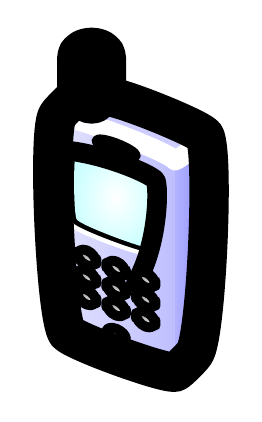
\begin{tikzpicture}[scale=0.25]
\begin{scope}[line join=round,looseness=0.25, line cap=round]
\begin{scope}
\clip [preaction={left color=blue!10, right color=blue!30}]
  (1/2,-1) to [bend left] (0,10)
  to [bend left] ++(1,1) -- ++(0,2)
  arc (180:0:3/4 and 1/2) -- ++(0,-2)
  to [bend left]  ++(5,-2) coordinate (A) to [bend left] ++(-1/2,-11)
  to [bend left] ++(-1,-1) to [bend left] cycle;
%
\path [left color=blue!30, right color=blue!50]
  (A) to [bend left] ++(0,-11) to[bend left] ++(-3/2,-2)
  -- ++(0,12);
%
\path [fill=blue!20, draw=white, line width=0.25cm]
  (0,10) to [bend left] ++(1,1) -- ++(0,2)
  arc (180:0:3/4 and 1/2) -- ++(0,-2)
  to [bend left]  (A) to [bend left] ++(-3/2,-5/4)
  to [bend right] cycle;
%
\draw [line width=0.25cm, fill=white]
  (9/8,21/2) arc (180:360:5/8 and 3/8) --
  ++(0,2.5) arc (0:180:5/8 and 3/8) -- cycle;
%
\draw [line width=0.25cm, fill=white]
  (9/8,13) arc (180:360:5/8 and 3/8);
%
\fill [white, shift=(225:0.5)]
  (1,17/2) to [bend left] ++(4,-7/4)
  to [bend left] ++(0,-7/2) to [bend left] ++(-4, 6/4)
  to [bend left] cycle;
%
\fill [black, shift=(225:0.25)]
  (1,17/2) to [bend left] ++(4,-7/4)
  to [bend left] ++(0,-7/2) to [bend left] ++(-4, 6/4)
  to [bend left] cycle;
%
\shade [inner color=white, outer color=cyan!20]
  (1,17/2) to [bend left] ++(4,-7/4)
  to [bend left] ++(0,-7/2) to [bend left] ++(-4, 6/4)
  to [bend left] cycle;
\draw [line width=0.25cm, shorten <=-0.5cm, shorten >=-0.5cm]
  (1,17/2) to [bend left] ++(4,-7/4)
  to [bend left] ++(0,-7/2);
%
\foreach \i in {1,2,3}
  \foreach \j in {1,2,3}
     \draw [line width=0.125cm, top color=gray,
       bottom color=white, yslant=-3/8, rounded corners=1cm/8]
         (\i*3/2-1/2,-\j+4) rectangle ++(1,3/4);
%
\draw [line width=0.125cm, top color=gray, bottom color=white, yslant=-3/8]
  (3,0) ellipse [x radius=1/2, y radius=1/3];
%
\draw [line width=0.125cm, top color=gray, bottom color=white, yslant=-3/8]
  (3,19/2) ellipse [x radius=1, y radius=1/4];
\end{scope}
\draw [line width=0.5cm]
  (1/2,-1) to [bend left] (0,10)
  to [bend left] ++(1,1) -- ++(0,2)
  arc (180:0:3/4 and 1/2) -- ++(0,-2)
  to [bend left]  ++(5,-2) to [bend left] ++(-1/2,-11)
  to [bend left] ++(-1,-1) to [bend left] cycle;
\end{scope}%

\end{tikzpicture}
}

\usepackage[acronym,nomain]{glossaries}
\usepackage{amsthm}
\usepackage{amssymb}
\usepackage{graphicx}
%\usepackage[center]{caption}
\usepackage{amsmath}
\usepackage{graphicx}
%\usepackage[chapter]{algorithm}
\usepackage{algpseudocode}

%\usepackage{algorithm}
%\usepackage{algorithmic}

\usepackage{dcolumn}
\usepackage{bigints}
\usepackage{psfig}

\usepackage{cite}
%\usepackage{subcaption}
 \usepackage{notoccite}
\usepackage{float}
%\usepackage{subfig}
%\usepackage{graphicx}
\usepackage{caption}
%\usepackage{longtable}

%\usepackage{color}   %May be necessary if you want to color links
%\usepackage{hyperref}
%\hypersetup{
%	breaklinks=true,
%    colorlinks=true, %set true if you want colored links
%    linktoc=all,     %set to all if you want both sections and subsections linked
%    linkcolor=black,  %choose some color if you want links to stand out
%}

\usepackage{hyperref}
\hypersetup{breaklinks=true, colorlinks=true, linkcolor=black, citecolor=black}

\hypersetup{urlcolor=black}


\DeclareMathOperator*{\argmin}{arg\;min}
\DeclareMathOperator*{\argmax}{arg\;max}
\newcounter{MYtempeqncnt}
%\usepackage{url}
%\usepackage{bbm}
%\usepackage{eufrak}
%%%%%%%%%%%%%
%\newtheorem{theorem}{Theorem}[chapter]
%\newtheorem{proposition}{Proposition}[chapter]
%\newtheorem{lemma}{Lemma}[chapter]
%\newtheorem{definition}{Definition}[chapter]


\newcommand\blfootnote[1]{%
\begingroup
\renewcommand\thefootnote{}\footnote{#1}%
\addtocounter{footnote}{-1}%
\endgroup
}




% \pagestyle{fancy}
% \renewcommand{\sectionmark}[1]{\markright{\thesection\ #1}}
% \fancyhf{}
 %\lhead{\fancyplain{}{\rightmark }}
 %\cfoot{\fancyplain{}{\thepage}}

%\doublespacing
%
%

%
%
\setlength{\parindent}{1em}
\setlength{\parskip}{1.25em}
\renewcommand{\baselinestretch}{1.35}

%\newtheorem{prop}{Proposition}
%-------------------------------------------------------------------
%\renewcommand{\contentsname}{Table of Contents}

%\makeatother
\usepackage{fancyhdr}
\usepackage{lipsum}% just to generate text for the example
%%%%%%%%%% To rename Table of Contents
\renewcommand{\contentsname}{Contents}
%%%%%%%%%%
%\flushbottom
%--------------------------------------------------------------------------
\raggedbottom                               % (Remove Unnecessary space b/w paragraphs)
%--------------------------------------------------------------------------
\begin{document}
\pagenumbering{roman}
% --------- Title and abstract etc the front matter -----------
% TITLE PAGE
\begin{titlepage}
\thispagestyle{empty}
\begin{center}
{\Large  \bf Incremental Security Enforcement for Underwater Drones}
\end{center}
% \vspace{-2.5em}
% \begin{center}
%  \textbf{COMMUNICATION SYSTEMS OVER FADING CHANNELS}
% \end{center}
 \vspace{0.1em}
\begin{center}
 \textbf{\textit{Thesis submitted to the}}
\end{center}
 \vspace{-3em}
\begin{center}
 \textbf{\textit{Indian Institute of Technology  Bhubaneswar}} 
\end{center}
 \vspace{-3em}
\begin{center}
 \textbf{\textit{for partial fulfillment of the requirements}} \\
 \textbf{\textit{for the degree of}} 
\end{center}
 \vspace{-1em}
\begin{center}
 \textbf{\textit{of}}
\end{center}
 \vspace{-1em}
\begin{center}
 \textbf{\large Bachelor and Master of Technology} \\
 \text{\small in} \\
 \textbf{\large Computer Science and Engineering}
\end{center}
 \vspace{-1em}
\begin{center}
 \textbf{\textit{by}}
\end{center}
 \vspace{-1em}
\begin{center}
 \large{\textbf{Vedanta Mohapatra}}
\end{center}
 \vspace{-1em}
\begin{center}
 Under the guidance of
\end{center}
 \vspace{-1em}
\begin{center}
 \textbf{Dr. Srinivas Pinisetty}
\end{center}
 \vspace{-1em}
\begin{center}

\includegraphics[scale=0.3]{iitbbs}
\end{center}
 \vspace{-1em}
\begin{center}
 \textbf{\small DEPARTMENT OF COMPUTER SC. \& ENGINEERING} \\
 \textbf{\small SCHOOL OF ELECTRICAL AND COMPUTER SCIENCES}
\end{center}
 \vspace{-3em}
\begin{center}
 \textbf{\small INDIAN INSTITUTE OF TECHNOLOGY BHUBANESWAR} 
\end{center}
 \vspace{-3em}
\begin{center}
 \textbf{November 2024}
\end{center}
 \vspace{-3em}
\begin{center}
 \copyright 2024 Vedanta Mohapatra. All rights reserved.
\end{center}
%\newpage
%\thispagestyle{empty}
\cleardoublepage

\end{titlepage}


\newpage
%%%%%%%%%%
\pagenumbering{roman}
 \addcontentsline{toc}{chapter}{Certification of Approval}
% Page 3 : Approval of the DSC
\thispagestyle{empty}
\begin{center}
	\textbf{\Large APPROVAL OF THE VIVA-VOCE BOARD}
\end{center}
\begin{flushright}
	DD/MM/YYYY
\end{flushright}
~~~Certified that the thesis entitled  \textbf{Incremental Security Enforcement for Underwater Drones}, submitted by \textbf{Vedanta Mohapatra} to the Indian Institute of Technology  Bhubaneswar, for the award of the degree of Doctor of Philosophy has been accepted by the external examiners and that the student has successfully defended the thesis in the viva-voce examination held today.
\begin{center}
	\begin{tabular*}{\textwidth}{@{\extracolsep{\fill}}cccccccc}
		&&&&&&&\\
		&&&&&&&\\
		\multicolumn{2}{c}{(Member of DSC)} && \multicolumn{2}{c}{(Member of DSC)} && \multicolumn{2}{c}{(Member of DSC)}\\
		&&&&&&&\\
		&&&&&&&\\
		\multicolumn{3}{c}{} &&& \multicolumn{3}{c}{(Supervisor)}\\
		% Comment the above line and uncomment the lower one if you have two supervisors
		% \multicolumn{3}{c}{(Supervisor)} &&& \multicolumn{3}{c}{(Supervisor)}\\
		&&&&&&&\\
		&&&&&&&\\
		\multicolumn{3}{c}{(External Examiner)} &&& \multicolumn{3}{c}{(Chairman)}\\
	\end{tabular*}
\end{center}

%% Page 4 : Blank
\newpage
%\thispagestyle{empty}
%\cleardoublepage

\addcontentsline{toc}{chapter}{Certificate}
% Page 5: Certificate on department letterhead
\thispagestyle{empty}
{~} % Buffer blank character to prevent horizontal underflow due to next \vspace
\vspace{10em} % Increase if the dept. letterhead requires more space
\begin{center}
	\textbf{\Large CERTIFICATE}
\end{center}
~~~This is to certify that the thesis entitled  \textbf{Write Thesis Title Here}, submitted by \textbf{Student Name} to Indian Institute of Technology  Bhubaneswar, is a record of bonafide research work under my supervision and I consider it worthy of consideration for the award of the degree of Doctor of Philosophy of the Institute.

\begin{tabular*}{\textwidth}{@{\extracolsep{\fill}}ll}
	&\\
	&\\
	&\\
	Date : & \textbf{Supervisor Name}\\
	& Designation\\
	& School of ******* Sciences \\
	& Indian Institute of Technology Bhubaneswar \\
	& Bhubaneswar, India \\
	% Comment the above line and uncomment the lower one if you have two supervisors
	% (Supervisor) & (Supervisor)\\
\end{tabular*}



%% Page 6 : Blank
\newpage
%\thispagestyle{empty}
%\cleardoublepage

\addcontentsline{toc}{chapter}{Declaration}
% Page 7: Declaration
\thispagestyle{empty}
\begin{center}
	\textbf{\Large DECLARATION}
\end{center}
I certify that
\begin{enumerate}[a.]
	\item the work contained in the thesis is original and has been done by myself under the general supervision of my supervisor.
	\item the work has not been submitted to any other institute for any degree or diploma.
	\item I have followed the guidelines provided by the institute in writing the thesis.
	\item I have conformed to the norms and guidelines given in the ethical code of conduct of the institute.
	\item whenever I have used materials (data, theoretical analysis, and text) from other sources, I have given due credit to them by citing them in the text of the thesis and giving their details in the references.
	\item whenever I have quoted written materials from other sources, I have put them under quotation marks and given due credit to the sources by citing them and giving required details in the references.
\end{enumerate}
\vspace{4em}
\begin{flushright}
	Student Name
\end{flushright}

%% Page 8 : Blank
\newpage


\addcontentsline{toc}{chapter}{Acknowledgments}
% Page 11 : Acknowledgment
\thispagestyle{empty}
\begin{center}
	\textbf{\Large Acknowledgments}
\end{center}

Write Acknowledgments Here


\vspace{3em}
\begin{flushright}
	Student Name
\end{flushright}

%%%%%%%%%%%%
\newpage
\chapter*{\centering Abstract}
\pagestyle{fancy}
\fancyhf{}
\rhead{\fancyplain{}{Abstract}}
\cfoot{\fancyplain{}{\thepage}}
\addcontentsline{toc}{chapter}{Abstract}

Cyber-Physical Systems (CPS) are integral to a wide range of critical applications, including autonomous vehicles, medical devices, and industrial automation. These systems merge physical processes with computational elements, creating complex environments that require stringent safety, security, and performance guarantees. However, the dynamic nature of CPS, combined with unpredictable environmental interactions, introduces significant challenges in ensuring system correctness at runtime. \\

\noindent Runtime enforcement plays a crucial role in addressing these challenges by monitoring and dynamically adjusting the system's behavior to adhere to predefined safety and security policies. Unlike static verification techniques, which may not account for unforeseen scenarios or evolving threats, runtime enforcement provides a real-time safeguard that detects and mitigates violations as they occur. This proactive approach enhances the resilience of CPS, ensuring they remain robust against internal faults and external attacks, ultimately protecting both the system's operation and its users. \\

\noindent In this work, we explore the use of compositional runtime enforcement in underwater robotic swarms, comparing its effectiveness against the traditional monolithic approach. The study focuses on applying runtime enforcement to a Multi-Robot Coverage Path Planning (MRCPP) algorithm, specifically designed for mapping underwater vegetation within a seagrass bed. By examining both approaches, we aim to assess their impact on the algorithm's performance, scalability, and adaptability in dynamic underwater environments.

\newpage
%\null\newpage
%\input{Abstract_2}
%\newpage\null\newpage
%\newpage
%%%%%%% To create single spacing in contents
%\singlespacing
\renewcommand{\baselinestretch}{1}
\pagestyle{fancy}
\fancyhf{}
%\rhead{\footnotesize{Contents}}
\rhead{\fancyplain{}{Contents}}
\cfoot{\fancyplain{}{\thepage}}
\tableofcontents


%\newpage\null
\newpage
\pagestyle{fancy}
\fancyhf{}
\rhead{\fancyplain{}{List of Figures}}
\cfoot{\fancyplain{}{\thepage}}
\addcontentsline{toc}{chapter}{List of Figures}
\listoffigures
%\newpage
%\addcontentsline{toc}{chapter}{List of Algorithms}
%\listofalgorithms
\newpage
\pagestyle{fancy}
\fancyhf{}
\rhead{\fancyplain{}{List of Tables}}
\cfoot{\fancyplain{}{\thepage}}
\addcontentsline{toc}{chapter}{List of Tables}
\listoftables
%\newpage\null\newpage
\newpage
%\fancyhf{}
\pagestyle{fancy}
\fancyhf{}
\rhead{\fancyplain{}{List of Abbreviations}}
\cfoot{\fancyplain{}{\thepage}}
%\null\newpage
\addcontentsline{toc}{chapter}{List of Abbreviations}
\chapter*{List of Abbreviations}
%\renewcommand{\arraystretch}{2}
%\begin{table}[ht] 
%\centering
%\begin{tabular}[l]{>{\bfseries}ll} 
%\addcontentsline{toc}{chapter}{List of Abbreviations}
\begin{longtable}[l]{>{\bfseries}ll} 
%\hline
%%%%% 1
%1G & First generation\\
%%%%% 2
%2G & Second generation\\
%%%% 5
5G & Fifth generation\\
%%%%%%%%%%%%% A
ABER & Average bit error rate\\
ADSL & Asymmetric digital subscriber line\\
AF & Amplify-and-forward \\
ASER &  Average symbol error rate\\
AWGN &   Additive white Gaussian noise\\
%%%%%%%%%%% B
BER & Bit error rate\\
BFSK & Binary frequency shift keying \\
BPSK & Binary phase shift keying \\




\end{longtable}
% \end{tabular} 
% \end{table} 


\newpage
%\null\newpage
\pagestyle{fancy}
\fancyhf{}
\rhead{\fancyplain{}{List of Symbols}}
\cfoot{\fancyplain{}{\thepage}}
\addcontentsline{toc}{chapter}{List of Symbols}
\chapter*{List of Symbols}

\begin{longtable}{ll}

%A
% $ F_A \left( \cdot ;\cdot ;\cdot;\cdot\right)$  &   Appell hypergeometric function \cite{RyzhikBook}.\\
$|\cdot|$          &    Absolute value\\
%B
$\left( {\begin{array}{*{20}c}
                   k\\ l\\ \end{array}} \right) $  & Binomial coefficient\\
$B(\cdot,\cdot)$ & Beta function\\
%C
$\Phi_2^{(n)}(\cdot)$ & Confluent form of the generalized Lauricella series\\
${}_1F_1(\cdot, \cdot;\cdot)$   & Confluent hypergeometric function  \\
$F_{X}(\cdot)$ & Cumulative distribution function of random variable $X$\\
%%%%%%% E
$\mathbb{E}[\cdot]$                  &      Expectation operator\\
$\text{exp}(\cdot)$                &     Exponential\\


\end{longtable}


























%\chapter*{List of Symbols}
% \begin{itemize}
% \item Basic arithmetic and calculus notations have standard definitions.
% \end{itemize}
% \section*{Elementary \& Special Functions}
% \begin{tabular}{p{2.5cm} p{12.5cm}}
% \hline\hline
% \textbf{Notation} & \textbf{Definition}\\
% \hline
% \hline
% \\
% $\Gamma(x)$ &  $= \displaystyle \int_{0}^{\infty} \textmd{e}^{-z}\, z^{x-1}\, dz$ denotes the Gamma function\\
% $\Upsilon(x,y)$ & $=\, \displaystyle \int_{0}^{y} \textmd{e}^{-t}\, t^{x-1}\, dt$ represents the lower incomplete Gamma function\\
% $\Gamma(x,y)$ & $=\,\, \displaystyle\int_{y}^{\infty} \textmd{e}^{-t}\, t^{x-1}\, dt$ represents the upper incomplete Gamma function\\
% $\mathcal{K}_{\upsilon}(x)$ & $= \displaystyle\frac{1}{2}\left(\frac{x}{2}\right)^{\upsilon} \int_{0}^{\infty} \frac{\textmd{e}^{-t-\frac{x^{2}}{4 t}}}{t^{\upsilon+1}} dt$ represents the modified Bessel function of the second kind of order $\upsilon$\\
% %$E_{n}(x)$ & $= \displaystyle\int_{1}^{\infty}\frac{\textmd{e}^{-x t}}{t^{n}}dt$ denotes the exponential integral function of order $n$\\
% $_{1}F_{1}(x,y;z)$ & $=\displaystyle\,\, \sum_{k=0}^{\infty}\frac{(x)_{k}}{(y)_{k}}\frac{z^{k}}{k!}$ represents the confluent hypergeometric function of first kind\\
% $_{2}F_{1}(x,y;w;z)$ & $= \displaystyle \sum_{k=0}^{\infty}\frac{(x)_{k}(y)_{k}}{(w)_{k}}\frac{z^{k}}{k!}$ represents the Gauss hypergeometric function\\
% %$I_{0}(x)$ & $= \displaystyle \sum_{k=0}^{\infty} \frac{(x/2)^{2 k}}{(k!)^{2}}$ denotes the zero-order modified Bessel function of the first kind\\
% %$\mathbb{B}(x,y)$ & $= \displaystyle \frac{\Gamma(x)\Gamma(y)}{\Gamma(x+y)}$ denotes the beta function\\
% $(x)_{k}$ & $= \displaystyle \frac{\Gamma(x+k)}{\Gamma(x)}$ denotes the Pochhammer symbol\\
% %$\ln(\cdot)$ & natural logarithm\\
% $Q_{z}(x,\phi)$ & $= \displaystyle \frac{1}{\pi}\int_{0}^{\phi}\exp\Big(-\frac{x^{2}}{2\sin^{2}\theta}\Big)\, d\theta$ represents Gaussian $Q$-function  \\
% \\
% \hline
% \end{tabular}
% %\newpage
% %\section*{Vectors and Matrices}
% %Let $\textbf{a}$ denotes the $N$$\times$$1$ complex vector.
% %\\
% %\\
% %\begin{tabular}{p{4cm} p{10cm}}
% %\hline\hline
% %\textbf{Notation} & \textbf{Definition}\\
% %\hline\hline
% %\\
% %$(\textbf{a})^{T}$ & transpose of $\textbf{a}$\\
% %$(\textbf{a})^{\dag}$ & conjugate of $\textbf{a}$\\
% %$(\textbf{\textbf{a}})^{H}$ & Hermitian transpose of $\textbf{a}$\\
% %$\mathbf{I}_{N}$ & $N\times N$ identity matrix\\
% %$\|\textbf{a}\|$ & Frobenius norm of $\textbf{a}$\\
% %\\\hline
% %\end{tabular}
% \section*{Probability \& Statistics}
% Let $X$ be a random variable, and $E$ be an arbitrary event.\\
% \\
% \begin{tabular}{p{4cm} p{10cm}}
% \hline\hline
% \textbf{Notation} & \textbf{Definition}\\
% \hline
% \hline
% \\
% $\mathbb{E}[\cdot]$ & Expectation operatot\\
% $\mathcal{L}[\cdot]$ & Laplace transform operator\\
% $\mathcal{L}^{-1}[\cdot]$ & Laplace transform operator\\
% $f_{X}(\cdot)$ & Probability density function of $X$\\
% %$f_{X|Y}(\cdot)$ & PDF of $X$ given $Y$\\
% $F_{X}(\cdot)$ & Cumulative distribution function of $X$\\
% $\textmd{Pr}[E]$ & Probability of event $E$\\
% % $X\sim\mathcal{CN}(\mu,\Omega)$ & $X$ is complex normal distributed with mean $\mu$ and variance $\Omega$\\
% %$X\sim \textmd{Nak}(m,\Omega)$ & $X$ is Nakagami distributed with fading severity parameter $m$ and average power $\Omega$\\
% \\
% \hline
% \end{tabular}

% \section*{Miscellaneous}
% \begin{tabular}{p{4cm} p{10cm}}
% \hline\hline
% \textbf{Notation} & \textbf{Definition}\\
% \hline\hline
% \\
% $|\cdot|$ & absolute value\\
% $\triangleq$ & equality by definition\\
% $\approx$ & approximate value\\
% $n!$ & factorial of $n$\\
% $(\textbf{a})^{*}$ & complex conjugate of $\textbf{a}$\\
% $\binom{n}{k}$ & binomial coefficient of $n$ choose $k$\\
% $G_{c, d}^{a, b}\left(\cdot\right)$ & represents the Meijer's-$G$ function\\
% $F_{A}^{(n)}(\cdot)$ & represents Lauricella hypergeometric function for $n$ variable\\
% $\arg \displaystyle\max_{i} b_{i}$ & index $i$ corresponding to the largest $b_{i}$\\
% $\arg \displaystyle\min_{i} b_{i}$ & index $i$ corresponding to the smallest $b_{i}$\\
% $\min(b_{1}, b_{2})$ & minimum of scalars $b_{1}$ and $b_{2}$\\
% $\max(b_{1}, b_{2})$ & maximum of scalars $b_{1}$ and $b_{2}$\\
% \\\hline
% \end{tabular}

\newpage
\pagenumbering{arabic}
%%%%%%%% To create double spacing
\doublespacing
\newpage
\pagestyle{fancy}
\renewcommand{\sectionmark}[1]{\markright{#1}}
\renewcommand{\chaptermark}[1]{\markboth{\chaptername~\thechapter~-~#1}{}}
\fancyhf{}
\rhead{\fancyplain{}{\rightmark}}
\lhead{\fancyplain{}{\leftmark }} 
\cfoot{\fancyplain{}{\thepage}}

  
\chapter{Introduction}
\graphicspath{{Chapter_1/Vector/}{Chapter_1/}}


Cyber-physical systems (CPSs) in the context of Underwater Unmanned Vehicles (UUVs) incorporate distributed embedded controllers that manage various physical processes critical to underwater operations \cite{lee2008cyber}. These systems have become an integral part of modern maritime applications, such as underwater exploration, environmental monitoring, military reconnaissance, and offshore infrastructure inspection. The security of CPSs controlling UUVs has emerged as a significant concern due to the critical nature of their applications. As these systems grow increasingly complex and interconnected, they become more susceptible to sophisticated cyberattacks \cite{loukas2015cyber,humayed2017cyber}.

In cyber-physical security attacks targeting UUVs, remote attackers can gain unauthorized control over the vehicle, interfere with its physical processes, and potentially cause catastrophic damage, including the loss of sensitive data, destruction of assets, or even risks to human life. For instance, malicious attacks on UUVs used in defense operations could lead to compromised missions or disruption of naval fleets. Recently, there were massive cyber attacks on Iran's nuclear facilities and government agencies\cite{ET2024Cyberattack}. Literature highlights notable CPS attacks, such as the Stuxnet worm damaging Iranian centrifuges \cite{langner2013kill}, the Maroochy Shire Water Services attack \cite{slay2007lessons}, and the German Steel Mill attack \cite{lee2014german}. Similarly, cyberattacks on autonomous drones and underwater vehicles have been documented, emphasizing the growing threat landscape for UUV operations \cite{yaacoub2020security}.

To address these challenges, formal runtime enforcement techniques\cite{enforceablesecpol,FalconeMFR11,RuntimeNonSafety,FMSD} have been proposed as reliable mechanisms for mitigating security concerns in CPSs, including UUVs \cite{ngo2015runtime,ligatti2009run,pearce2019securing}. The research domain known as runtime verification (RV)\cite{LeuckerS08jlap} focuses on dynamically verifying a set of desirable policies during the execution of a ``black-box'' system. An RV monitor observes the system's execution trace without interfering and determines whether it satisfies or violates specific policies.

Runtime enforcement (RE), an active counterpart to passive runtime verification, provides a mechanism to guarantee the adherence to desired policies during system execution. In RE mechanisms, an enforcer is designed to monitor a black-box system and take corrective actions when policy violations are detected. For UUVs, such actions are critical for ensuring mission safety and security. Evasive measures include blocking harmful actions \cite{enforceablesecpol}, modifying input sequences by suppressing or adding actions \cite{RuntimeNonSafety}, or buffering inputs until they can be safely executed \cite{FalconeMFR11,FMSD}. These techniques are particularly relevant for UUVs operating in dynamic and unpredictable underwater environments, where maintaining system safety and security is paramount.

% \begin{figure}
% \begin{tikzpicture}[->,shorten >=1pt,auto,node distance=2.5cm,semithick,initial where=left]

% \tikzstyle{every node}=[font=\small]

% \tikzstyle{good state}=[circle,thick,draw=blue!75,fill=blue!20,minimum size=5mm,accepting]
% \tikzstyle{bad state}=[circle,thick,draw=red!75,fill=red!20,minimum size=3mm]
% \tikzstyle{dead state}=[rectangle,thick,draw=red!75,fill=red!20,minimum size=5mm]

% \node[initial,good state] (l0) {$l_0$};
% \node[good state]         (l1) [right=3 of l0] {$l_1$}; %[right of=l0] {$l_1$};
% \node[bad state]        (l2) [below=1cm of l1] {$l_2$};

% \path (l0) edge node [align=center]  {$ A_{G_1} $ and ($ b_1 $ and $ c_1 $) :\\ $ a_1=1 $ }( l1)
% edge [loop above] node [align=center] {$ B_{G_1} $: $ b_1=1 $\\$C_{G_1}$: $ c_1=1 $}(l0)  
% edge [loop below] node [align=center] {$ \Sigma \setminus \{A_{G_1}, B_{G_1}, C_{G_1}\} $}(l0)  
% edge [bend right=20] node [align=center] [anchor=south east, yshift=-40pt, xshift=40pt] {$ A_{G_1} $ and ($ !b_1 $ or $ !c_1$):\\ $ A_{G_1}=0$;}(l2)          

% (l1) edge  [loop right] node {$ A_{G_1} $} (l1)
% edge node [align=center] {($ B_{G_1}$: $ B_{G_1}=0$)  or\\ ($ C_{G_1} $: $ C_{G_1}=0$)} (l2)
% edge [loop above] node [align=center] {$ \Sigma \setminus \{A_{G_1}, B_{G_1}, C_{G_1}\} $}(l0)

% (l2) edge [loop right] node {$\Sigma$} (l2);

% \end{tikzpicture}
% \captionof{figure}{VDTA specifying the constraint: ``\textit{Peer A can undertake a research project only after it has been approved by peer \{B, C\}}".}
% \label{fig:vdta}
% \end{figure}


%%%%%%%%%%%%%%%%%
%%%%%%%%%%%%%%%%%%
%%%%%% Chapter 1 Section 1
%%%%%%%%%%%%%%%%%
%%%%%%%%%%%%%%%%%%
\section{Literature Survey}
\rhead{Literature Survey}
\label{LiteratureSurvey}

Runtime verifiers are extensively used in underwater drone systems to ensure operational accuracy and detect malicious attacks. For example, similar to the Argus framework \cite{adepu2016argus}, external intelligent controllers can monitor the physical processes of underwater drones, enforcing policies such as depth, velocity, and collision avoidance based on operational invariants. Alternatively, runtime verification can be embedded directly within controllers \cite{adepu2017design}, enabling real-time detection and reporting of anomalies or rule violations.

Specific cyberattacks on underwater drones include jamming, injection, and data alteration. To counter such threats, various runtime enforcement (RE) mechanisms have been proposed. For instance, Baird et al. \cite{baird2022runtime} modeled these attacks in a simulated drone system and developed runtime enforcers. Additionally, resilient control methods, such as those by Sun et al. \cite{sun2019resilient}, use dual-mode algorithms to counter denial-of-service (DoS) attacks in CPS environments.

Traditional RE approaches (e.g., \cite{FalconeMFR11,RuntimeNonSafety}) rely on buffering or editing event sequences but are less suitable for reactive systems like underwater drones, where actions must occur instantaneously. Recent frameworks such as shields \cite{BloemKKW15,spin17} allow for bi-directional enforcement by transforming outputs dynamically while maintaining system reactivity.

Our research builds on these principles, proposing a compositional RE framework for underwater drones. This approach allows enforcers to be incrementally added in series, enabling seamless integration of new security policies as threats evolve, without disrupting the existing system. This compositionality ensures flexibility and adaptability in securing underwater drones against emerging challenges.

\section{Motivation}
\rhead{Motivation}
\label{Motivation}

In practice, runtime security policies for underwater drones evolve over time as cyberattacks emerge and software systems grow more complex. Understanding the secured and unsecured behaviors of such systems also evolves with advancements in their applications. Underwater drones, deployed in diverse areas such as ocean exploration, environmental monitoring, and military surveillance, often require new and more sophisticated security policies alongside existing ones. Ensuring the security of these systems is inherently incremental: as new threats are identified, new security measures and patches are implemented to address them.

Consider an underwater drone swarm as an example of a cyber-physical system (CPS). These drones operate with distributed controllers that manage their physical processes, such as depth, orientation, and velocity. They are frequently employed to monitor marine ecosystems, detect underwater anomalies, and transport goods in aquatic environments. Each drone operates within specific underwater zones and must adhere to restrictions in spatial movement to avoid collisions, boundary violations, or excessive energy consumption. However, the increasing use of underwater drones has also introduced new security vulnerabilities, exposing them to cyberattacks such as spoofing, jamming, and unauthorized access. Research has highlighted the necessity of augmenting existing security frameworks with more robust policies to protect against such threats.

Incremental enforcement of security policies becomes essential in this context, especially as new challenges or attack vectors emerge. Instead of synthesizing a monolithic enforcer from scratch for every new policy, incremental enforcement allows for the addition of new policies without altering or revalidating the existing ones. This approach is particularly relevant when the underlying system is designed to handle dynamic, evolving environments, as is often the case with underwater drones. Monolithic enforcement methods face significant drawbacks, including high costs of redevelopment, re-certification, and risks of disrupting previously concealed or secret policies. These issues underscore the importance of designing enforcers capable of incorporating new policies without requiring knowledge of previously enforced ones.

This work focuses on studying incremental enforcement mechanisms for underwater drones, utilizing approaches like those proposed in prior research (e.g., \cite{spin17, 10047915}), which are suitable for reactive CPS systems. In this context, the underwater drones are modeled as synchronous reactive systems. These systems continuously interact with their environment, with execution consisting of steps where the system reads inputs, performs reactions, and computes outputs. Such modeling ensures that new security policies can be incrementally added and enforced without compromising the system's overall integrity or performance.
  \newpage 
%  %\newpage\null\newpage
  
\chapter{Runtime Enforcement Framework}
\graphicspath{{Chapter_2/Vector/}{Chapter_2/}}

Before delving into the specific details of the runtime enforcement framework, it is important to first establish some foundational concepts and the necessary notation. This section introduces key elements such as edit functions, runtime enforcement for synchronous programs, and the framework for policies defined as safety automata. Understanding these preliminaries will provide the necessary context for the subsequent discussions on the design and application of runtime enforcement mechanisms in various program types.


\section{Preliminaries and Notation}
\rhead{Preliminaries and Notation}
\label{prelim}

In this section, we introduce the notations and the safety automaton formalism used to define policies to be monitored and enforced. We also briefly recall the RE problem for synchronous programs (all the constraints that an enforcer should fulfill). 

A finite word over a finite alphabet $\Sigma$ is a finite sequence $\sigma = a_1\cdot a_2\cdots a_n$ of members of $\Sigma$, and $\Sigma^*$ denotes the set of finite words over $\Sigma$.
Considering a finite word $\sigma$, its length is denoted as  $|\sigma|$.
$\epsilon_\Sigma$ is used to denote the empty word over $\Sigma$ is denoted by $\epsilon_\Sigma$, or $\epsilon$ (when the context makes it evident).
Given two words $\sigma$ and $\sigma'$, their {\em concatenation} is indicated as $\sigma\cdot \sigma'$. 
A word $\sigma'$ is a {\em prefix} of a word $\sigma$, represented as $\sigma' \pref \sigma$, whenever a word $\sigma''$ is present such that $\sigma = \sigma'\cdot \sigma''$; $\sigma$ is called an \emph{extension} of $\sigma'$.

A reactive system with a finite {ordered} sets of Boolean inputs $I= \{i_1, i_2,\cdots,i_n\}$ and Boolean outputs $O= \{o_1, o_2,\cdots,o_m\}$ is considered.
$\Sigma_I=2^I$ denotes the input alphabet, $\Sigma_O=2^O$ denotes the output alphabet, and the input-output alphabet is $\Sigma= \Sigma_I \times \Sigma_O$.
A bit-vector/complete monomial will be used to represent each input (resp. output) event.
For example, let us consider $I=\{P, Q\}$.
Then, the input $\{P\} \in \Sigma_I$ is denoted as  $10$, while $\{Q\} \in \Sigma_I$ is denoted as $01$ and  $\{P, Q\} \in \Sigma_I$ is denoted as $11$.
A reaction (or input-output event) has the following structure: $(x_i, y_i)$, where $x_i \in \Sigma_I$ and $y_i \in \Sigma_O$.

Given  $\sigma= (x_1,y_1)\cdot(x_2,y_2)\cdots(x_n,y_n) \in \Sigma^*$ which is an input-output word, the input word acquired from $\sigma$ is $\sigma_I = x_1 \cdot x_2 \cdots x_n \in \Sigma_I$, which is a projection that ignores outputs and is based on inputs.
Similarly, the output word obtained from $\sigma$ is $\sigma_O = y_1 \cdot y_2 \cdots y_n \in \Sigma_O$ is the projection on outputs ignoring inputs.

\ignore{
	An execution $\sigma$ of a synchronous program $\calP$ is an infinite sequence of input-output events $\sigma\in\Sigma^{\omega}$, and the \emph{behavior} of a synchronous program $\calP$ is denoted as $\exec(\calP)\subseteq \Sigma^{\omega}$.
	The \emph{language} of $\calP$ is denoted by $\cal{L}(\cal{P})$ = $\{\sigma \in \Sigma^* | \exists \sigma' \in \exec(\calP) \wedge \sigma \pref \sigma'\}$ i.e. $\cal{L}(\cal{P})$ is the set of all finite prefixes of the sequences in $\exec(\calP)$.
}

A policy denoted as $\varphi$ (over $\Sigma$) represents a set $\calL(\varphi)\subseteq \Sigma^{*}$.
%A program $\calP \models \varphi$ iff $\calL(\calP) \subseteq  \calL(\varphi)$.
Given a word $\sigma \in \Sigma^*$, $\sigma \models \varphi$ iff $\sigma\in\calL(\varphi)$.
A {policy} $\varphi$ is {\em prefix-closed} if all prefixes of all words from
$\calL(\varphi)$ are also in $\calL(\varphi)$: $\calL(\varphi) = \{w\;|\;\exists w'\in\calL(\varphi): w\pref w'\}$.
Prefix-closed policies are the focus of this study.
Policies are formalized as safety automata, which we define next in
this section.



Synchronous programming languages~\cite{BenvenisteCEHLd03} are ideal for developing synchronous reactive systems.
They express safety properties via observers ~\cite{HalbwachsLR94}, which are statically verified (using model checking). Safety automata are analogous to observers but are enforced at runtime.

\begin{definition}[Safety Automaton]
	\label{def:SA}
	A \emph{safety automaton} (SA) $\calA =(Q, q_0, q_v, \Sigma, \xrightarrow{})$ is a tuple, where $Q$ denotes the set of states, known as \emph{locations}, $q_0 \in Q$ is a distinct starting location, $q_v \in Q$ is a distinct non-accepting (violating) location, the alphabet is $\Sigma=\Sigma_I\times\Sigma_O$, and the transition relation is $\xrightarrow{} \subseteq Q \times \Sigma \times Q$.
	Except for  $q_v$, all the other locations are accepting  (i.e., all the locations in $Q \setminus \{q_v\}$).
	Location $q_v$ is a distinct violating (trap) location, thus no transitions in $\xrightarrow{}$ from $q_v$ to a location in $Q \setminus \{q_v\}$.
	%
	Whenever there exists $(q, a, q') \in \xrightarrow{}$, we denote it as $q \xrightarrow{a} q'$.
	%
	Relation $\xrightarrow{}$ is extended to words $\sigma \in \Sigma^*$ by noting
	$q \xrightarrow{\sigma . a} q'$ whenever there exists $q''$ such that $q
	\xrightarrow{\sigma} q''$ and $q'' \xrightarrow{a} q'$.
	A location $q\in Q$ is reachable from $q_0$ if there exists a word $\sigma \in \Sigma^*$ such that $q_0
	\xrightarrow{\sigma} q$.
\end{definition}

An SA $\calA = (Q, q_0, q_v, \Sigma, \xrightarrow{})$ is \textit{deterministic} if $\forall
q \in Q, \forall a \in \Sigma, (q \xrightarrow{a} q' \land q \xrightarrow{a}
q'') \implies (q' = q'')$.
$\mathcal{A}$ is \textit{complete} if $\forall q \in Q, \forall a \in \Sigma, \exists q' \in Q, q \xrightarrow{a} q'$.
A word $\sigma$ is \textit{accepted} by $\mathcal{A}$ if there exists $q \in Q \setminus \{q_v\}$ such that $q_0
\xrightarrow{\sigma} q$.
The set of all words accepted by $\mathcal{A}$ is denoted as $\mathcal{L}(\mathcal{A})$.

\begin{remark}
	We can first determinize and complete a non-deterministic or incomplete automaton provided by the user.
	We further assume that $Q$ has no (redundant) locations that are
	unreachable from $q_0$. Hence, in the rest of this work, $\varphi$ is a safety policy specified as deterministic and complete SA $\calA_\varphi = (Q, q_0, q_v, \Sigma, \xrightarrow{})$. 
\end{remark}

The enforcer must first alter inputs from the environment in each step according to policy $\varphi$ specified as SA $\calA_\varphi$ according to the causality requirement.
As a result, we must examine the input policy obtained by projecting
on inputs from $\calA_\varphi$. 

\begin{definition}[Input SA $\calA_{\varphi_I}$]
	\label{def:inp:prop:proj:def}
	Given $\varphi\subseteq\Sigma^*$, specified as SA $\calA_{\varphi}=(Q, q_0, q_v, \Sigma, \rightarrow)$,  by discarding outputs on the transitions, input SA $\calA_{\varphi_I}=(Q, q_0, q_v, \Sigma_I, \rightarrow_I)$ is derived from $\calA_{\varphi}$.That is, for every transition  $q \xrightarrow{(x,y)} q' \in \rightarrow$ where $(x,y) \in \Sigma$, there is a transition  $q \xrightarrow{x} q' \in \rightarrow_I$, where $x \in \Sigma_I$.
	$\calL(\calA_{\varphi_I})$ is represented as $\varphi_I \subseteq \Sigma_I^*$.
\end{definition}

\begin{figure}[htb]
	%
	\centering
	\hspace{-4.0em}
	\subfloat[SA $\calA_{P}$. \label{fig:prop1}]{
		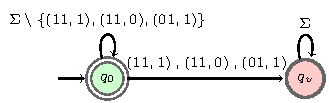
\includegraphics[scale=1]{fig/propAutomaton2-crop2.pdf}
	}
	%\hspace{1.0em}
	\subfloat[Input SA from $\calA_{P}$. \label{fig:prop1Inp}]{
		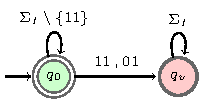
\includegraphics[scale=1]{fig/propAutomatonprojI2-crop2.pdf}
	}
	\caption[]{SA (left), and its input SA (right). \footnotemark}
	\label{fig:prop:inpProj}
\end{figure}

\footnotetext{Here, $\Sigma = \{(00,0), (00,1), (01,0), (01,1), (10,0), (10,1), (11,0), \\ (11,1)\}$. So $\Sigma \setminus \{(11,1), (11,0), (01,1)\}$ = $\{(00,0), (00,1), (01,0), (10,0), (10,1)\}$.}
%%%%%%%%%%%%%%%%%%%%%%%%%%%%%
%
%%%%%%%%%%%%%%%%%%%%%%%%%%%%%
\begin{example}[Example policy defined as SA and its input SA]
	\label{eg:prop}
	%%%%%%%%%%%%%%%%%%%%%%%%%%%%%
	Consider $I= \{B,Q\}$ and $O = \{ X \}$.
	Let us consider the policy: \textit{$P$: ``B and Q can't happen at the same time, and Q and X can't happen at the same time''}.
	Policy $P$ is defined by the safety automaton in Figure~\ref{fig:prop1}.
	The input SA for the SA in Figure~\ref{fig:prop1} defining policy $P$ is shown in Figure~\ref{fig:prop1Inp}.
	Though the SA $\calA_\varphi$ is deterministic, the input SA $\calA_{\varphi_I}$ may be non-deterministic. This is the case with the considered example as shown in Figure~\ref{fig:prop1Inp}.
\end{example} 

\begin{lemma}
	\label{lem:inputProp}
	%%%%%%%%%%%%%%%%%%%%%%%%%%%%%
	Consider $\calA_{\varphi_I}=(Q, q_0, q_v, \Sigma_I, \rightarrow_I)$ be the input automaton derived from $\calA_{\varphi}=(Q, q_0, q_v, \Sigma, \rightarrow)$. The policies we have are as follows:
	\squishlist
	\item[1] $\forall (x,y) \in \Sigma, \forall q, q'\in Q: q\xrightarrow{(x,y)}q' \implies q \xrightarrow{x}_I q'$.
	\item[2] $\forall x \in \Sigma_I, \forall q, q'\in Q: q \xrightarrow{x}_I q' \implies \exists y\in\Sigma_O: q\xrightarrow{(x,y)}q'$.
	\squishend
\end{lemma}
Lemma~\ref{lem:inputProp} is an immediate consequence from Definitions~\ref{def:SA} and~\ref{def:inp:prop:proj:def}.
Policy 1 states that if there is a transition from state $q\in Q$ to state $q' \in Q$  in the automaton $\calA_\varphi$ upon input-output event $(x,y)\in \Sigma$, then there is a transition from state $q$ to state $q'$ in the input automaton $\calA_{\varphi_I}$ upon the input event $x\in\Sigma_I$.
Policy 2 states that if there is a transition from state $q\in Q$ to state $q' \in Q$ upon input event $x\in\Sigma_I$, then there must be an output event $y\in\Sigma_O$ s.t. there is a transition from state $q$ to state $q'$ upon event $(x,y)$ in the automaton $\calA_\varphi$. 
%%%%%%%%%%%%%%%%%%%%%%%%%%%%%
\begin{definition}[Product of SA]
	\label{def:product}
	Given two SA $\calA_{\varphi_1}=(Q^1, q^1_0, q^1_v, \Sigma, \rightarrow_1)$, and $\calA_{\varphi_2}=(Q^2, q^2_0, q^2_v, \Sigma, \rightarrow_2)$, their product SA $\calA_{\varphi_1} \times \calA_{\varphi_2} = (Q, q_0, q_v, \Sigma, \rightarrow)$ where $Q = Q^1 \times Q^2$, $q_0 = (q^1_0, q^2_0)$, $q_v =  (q^1_v, q^2_v)$, and the transition relation $\rightarrow \subseteq Q \times \Sigma \times Q$ with $((q^1, q^2), a, (q'^1, q'^2)) \in \rightarrow$  if  $(q^1, a, q'^1) \in \rightarrow^1$ and  $(q^2, a, q'^2) \in \rightarrow_2$. 
	
	In the product SA $\calA_{\varphi_1} \times \calA_{\varphi_2}$, all the locations in $(Q^1\times q^2_v) \cup (q^1_v \times Q^2)$ are trap locations. 
	All the outgoing transitions from these locations can be replaced with self-loops, and all such locations can be merged into a single violating location labeled as $q_v$. Any outgoing transition from a location in $Q \setminus (Q^1\times q^2_v) \cup (q^1_v \times Q^2)$ to a location in $(Q^1\times q^2_v) \cup (q^1_v \times Q^2)$ goes to $q_v$ instead.  
	
	
	% \SP{TODO: To expand/clarify reg violating loc in the product !}
\end{definition}

The product of SAs is useful to enforce multiple policies using the monolithic approach by first constructing a product of the given SAs. Given two deterministic and complete SAs $\calA_{\varphi_1}$ and $\calA_{\varphi_2}$, the product SA $\calA_{\varphi_1} \times \calA_{\varphi_2}$ is deterministic and complete which recognizes the language 
$\calL(\calA_{\varphi_2}) \cap \calL(\calA_{\varphi_2})$.
%\SP{We may add a couple of lines of expl. of the product def later if space permits.}
%%%%%%%%%%%%%%%%%%%%%%%%%
%%%%%%%%%%%%%%%%%%%%%%%%%%%%
\subsection{Edit Functions}
\label{sec:prelim:re}
%%%%%%%%%%%%%%%%%%%%%%%%%%%%
Let us consider policy $\varphi\subseteq\Sigma^*$, specified as SA $\calA_{\varphi}=(Q, q_0, q_v, \Sigma, \rightarrow)$, and SA $\calA_{\varphi_I}=(Q, q_0, q_v, \Sigma_I, \rightarrow_I)$ derived from $\calA_{\varphi}$ by discarding outputs.
The enforcer utilizes the following  $\editI$ (resp. $\editO$), for editing input (resp. output) events (when required), as per the policy $\varphi_I$ (resp. $\varphi$).
%
%
\squishlist
\item {{\boldmath$\editI(\sigma_I)$}}: Given $\sigma_I\in\Sigma_I^*$, $\editI(\sigma_I)$ is the set of input events $x \in \Sigma_I$ s.t. the word obtained by concatenating $x$ after $\sigma_I$ satisfies policy $\varphi_I$. Formally,
\[\editI(\sigma_I) = \{ x\in \Sigma_I: \sigma_I \cdot x \models \varphi_I \}.\]
%
When we consider the SA $\calA_{\varphi_I}=(Q, q_0, q_v, \Sigma_I, \rightarrow_I)$,
the members in $\Sigma_I$ that allow to reach a state in $Q\setminus \{q_v\}$ from a state $q\in Q\setminus \{q_v\}$ is defined as:
\[\editIaut(q) = \{x\in \Sigma_I: q \xrightarrow{x}_I q' \wedge q' \neq q_v \}. \]
%
Let us\blue{,} for example\blue{,} consider the SA in Figure~\ref{fig:prop1Inp} derived from the SA in Figure~\ref{fig:prop1} by projecting on inputs.
If we consider $\sigma= (10,0)\cdot(01,1)$, we have $\sigma_I= 10\cdot01$.
Then, $\editI(\sigma_I) = \Sigma_I\setminus\{11\}$.
Moreover, $q_0 \xrightarrow{10\cdot01}_I q_0$, and $\editIaut(q_0) = \Sigma_I\setminus\{11\}$.

%
%For example, consider the automaton in Figure~\ref{fig:prop1Inp} obtained from the automaton in Figure~\ref{fig:prop1} by ignoring outputs.
%Let $\sigma= (11,00)\cdot(10,11)$, and thus $\sigma_I= 11\cdot10$.
%Then, $\editI(\sigma_I) = \Sigma_I$.
%Also, $q_0 \xrightarrow{11\cdot10}_I q_0$, and $\editIaut(q_0) =  \Sigma_I$.
%
%
If $\editIaut(q)$ is non-empty, then $\randEditIaut(q)$ returns an element (chosen randomly) from $\editIaut(q)$ and is undefined if $\editIaut(q)$ is empty.
%
\item {\boldmath$\editO(\sigma, x)$}:~~Consider an input event $x\in\Sigma_I$, and an input-output word $\sigma\in\Sigma^*$. We have $\editO(\sigma, x)$, the set of output events $y$ in $\Sigma_O$ s.t. the input-output word obtained by concatenating $\sigma$ followed by $(x,y)$ (i.e., $\sigma\cdot (x,y)$) satisfies policy $\varphi$. Formally,
\[\editO(\sigma,x) = \{y \in \Sigma_O: \sigma \cdot (x,y) \models \varphi \}.\]
%
When we consider the automaton $\calA_{\varphi}=(Q, q_0, q_v, \Sigma, \rightarrow)$ specifying policy $\varphi$, and an input event $x\in\Sigma_I$,
the set of output events $y$ in $\Sigma_O$ permitting to reach a state in $Q\setminus \{q_v\}$ from a state $q\in Q\setminus \{q_v\}$ with $(x,y)$ is defined as:
\[\editOaut(q,x) = \{y \in \Sigma_O: q \xrightarrow{(x,y)} q' \wedge q' \neq q_v \}. \]
\noindent
%
For example, consider policy $P$ defined by the automaton in Figure~\ref{fig:prop1}.
We have $\editOaut(q_0, 01) = \{0\}$.

If $\editOaut(q,x)$ is not empty, then $\randEditOaut(q, x)$ returns a random element from $\editOaut(q,x)$, and if $\editOaut(q,x)$ is empty $\randEditOaut(q, x)$ is undefined.
%
%For example, consider property $S_1$ defined by the automaton in Figure~\ref{fig:prop1}.
%We have $\editOaut(q_0, 11) =  \{00,01\}$.
%
%\item {\boldmath$\randEditI(\sigma_I)$:}~~ Given $\sigma_I\in\Sigma_I^*$ if $\editI(\sigma_I)$ is non-empty, then $\randEditI(\sigma_I, x)$ returns an element (chosen randomly) from $\editI(\sigma_I)$ , and is undefined if $\editI(\sigma_I)$ is empty.
%
%\item {\boldmath$\randEditO(\sigma,x)$:}~~ Given $\sigma\in\Sigma^*$, and $x\in\Sigma_I$,  if $\editO(\sigma,x)$ is non-empty, then $\randEditO(\sigma,x)$ returns an element (chosen randomly) from $\editO(\sigma,x)$ , and is undefined if $\editO(\sigma,x)$ is empty.
%
\ignore{
	\item {\boldmath$\minEditI(\sigma_I, x)$:}~~ Given $\sigma_I\in\Sigma_I^*$ and $x\in\Sigma_I$, if $\editI(\sigma_I)$ is non-empty, then $\minEditI(\sigma_I, x)$ returns an event from $\editI(\sigma_I)$ with minimal distance\footnote{Distance between two events belonging to the same alphabet is the number of bits that differ in both the events.} w.r.t $x$, and is undefined if $\editI(\sigma_I)$ is empty.
	
	Consider the automaton $\calA_{\varphi_I}=(Q, q_0, q_v, \Sigma_I, \rightarrow_I)$.
	Given $q\in Q$ and $x \in \Sigma_I$, if $\editIaut(q)$ is non-empty, then $\minEditIaut(q, x)$ returns an event from $\editIaut(q)$ with minimal distance w.r.t $x$, and is undefined if $\editIaut(q)$ is empty.
	\TODO{SR@All: Currently $\randEditI$/$\randEditO$ are used in the algorithm. We could use $\minEditI$/$\minEditO$ instead or we can make a remark about minimal editing. Otherwise to suppress from prelim if not used. }
	\item {\boldmath$\minEditO(\sigma, x, y)$:}~~ Given $\sigma\in\Sigma^*$, $x\in\Sigma_I$ and $y\in\Sigma_O$, if $\editO(\sigma,x)$ is non-empty, then $\minEditO(\sigma, x, y)$ returns an event from $\editO(\sigma,x)$ with minimal distance w.r.t $y$, and is undefined if $\editO(\sigma, x)$ is empty.
	
	Consider the automaton $\calA_{\varphi}=(Q, q_0, q_v, \Sigma, \rightarrow)$.
	Given $q\in Q$, $x\in\Sigma_I$ and $y\in\Sigma_O$, if $\editOaut(q,x)$ is non-empty, then $\minEditOaut(q, x, y)$ returns an event from $\editOaut(q,x)$ with minimal distance w.r.t $y$, and is undefined if $\editOaut(q,x)$ is empty.
}
%
\squishend

\subsection{Runtime Enforcement for Synchronous Programs}
\label{sec:problemDef}
%%%%%%%%%%%%%%%%%%%%%%%%%%%%%%%%

In this section, we briefly recall the RE problem for synchronous programs from \cite{spin17}.
{In this setting, that we also consider in this work, as illustrated in Figure~\ref{fig:intro-context}, an enforcer monitors and corrects both inputs and outputs of a synchronous program according to a given safety policy $\varphi\subseteq\Sigma^*$.}

The model hypothesizes that the black-box synchronous program can be called using a custom function call called $ptick$ that is called just once during each reaction / synchronous step.
%
We can formally consider $\ptick$ as a function from $\Sigma_I$  to  $\Sigma_O$ that accepts a bit vector $x \in \Sigma_I$ and returns a bit vector $y \in \Sigma_O$.

An enforcer for the policy $\varphi$ can only alter an input-output event when it's absolutely essential; it can't block, postpone, or suppress events.
Let's remember the two functions $\editI$ and $\editO$ from Section~\ref{sec:prelim}, which the enforcer for $\varphi$ uses to edit the current input (or output) event according to the policy $\varphi$.
An enforcer may be thought of as a function that modifies input-output words at a high level.
An enforcement function for the policy $\varphi$ takes an input-output word over $\Sigma$ as input and produces an input-output word over $\Sigma$ that conforms to $\varphi$ as output.
%

We reproduce  from \cite{spin17} and briefly discuss,  Definition \ref{def-E-func-constraints} of the constraints that an enforcer for any given policy $\varphi$ should satisfy:
%%%%%%%%%%%%%%%%%%%%%%%%%%%%%%%%%%%%%%%%%%%%%%
\begin{definition}[Enforcer for $\varphi$]
	\label{def-E-func-constraints}
	An {\em enforcer} for a given policy $\varphi\subseteq\Sigma^*$ is a function $\ef: \Sigma^*\rightarrow \Sigma^*$ satisfying the following constraints:
	%
	
	\noindent
	{\bf Soundness}
	\begin{equation}
		\tag{\bf Snd}\label{eq:snd}
		\forall \sigma \in \Sigma^*: \ef(\sigma) \models \varphi.
	\end{equation}
	%
	{\bf Monotonicity}
	\begin{equation}
		\tag{\bf Mono}\label{eq:mono}
		\forall \sigma, \sigma' \in \Sigma^*: \sigma\pref \sigma' \Rightarrow \ef(\sigma) \pref \ef(\sigma').
	\end{equation}
	%
	{\bf Instantaneity}
	\begin{equation}
		\tag{\bf Inst}\label{eq:inst}
		\forall \sigma \in \Sigma^*: |\sigma| =  |\ef(\sigma)|.
	\end{equation}
	%
	{\bf Transparency}
	\begin{equation}
		\tag{\bf Tr}\label{eq:tr}
		\begin{array}{ll}
			\forall \sigma\in \Sigma^*, \forall x \in \Sigma_I,\forall y \in \Sigma_O:\\
			~~~~~\ef(\sigma)\cdot(x,y)\models \varphi \implies \\ \ef(\sigma\cdot(x,y)) = \ef(\sigma)\cdot(x,y).
		\end{array}
	\end{equation}
	%
	{\bf Causality}
	\begin{equation}
		\tag{\bf Cau}\label{eq:ca}
		\begin{array}{ll}
			\forall \sigma \in \Sigma^*, \forall x \in \Sigma_I,\forall y \in \Sigma_O,\exists x' \in \editI(\ef(\sigma)_I), \\
			~~~~\exists y' \in \editO(\ef(\sigma), x'): \ef(\sigma\cdot(x,y))= \\ \ef(\sigma)\cdot(x',y').
			%\wedge \ef(\sigma)\cdot(x',y')\models \varphi.
		\end{array}
	\end{equation}
	%
\end{definition}
%%%%%%%%%%%%%%%%%%%%%%%%%%%%%%%%%%%%%%%%%%%%%%%%%%%%
The enforcer releases the input-output sequence $\ef(\sigma)$ as output after reading the input-output sequence $\sigma$, and $\ef(\sigma)_I \in \Sigma_I^*$ is the projection on the inputs.
Note that $\editI(\ef(\sigma)_I)$ returns a set of input events in $\Sigma_I$, s.t. $\ef(\sigma)_I$  (which is the input alphabet projection of the input-output word $\ef(\sigma)$)  followed by any event from $\editI(\ef(\sigma)_I)$ satisfies $\varphi_I$.
$\editO(\ef(\sigma), x')$ returns a set of output events in $\Sigma_O$, such that for any event $y$ in $\editO(\ef(\sigma), x')$, $\ef(\sigma)\cdot(x',y)$ satisfies $\varphi$.
%
\squishlist
\item Soundness $(\ref{eq:snd})$ states that the output of the enforcer $\ef(\sigma)$ must satisfy $\varphi$ for any word $\sigma\in\Sigma^*$.
%%
\item Monotonicity $(\ref{eq:mono})$ specifies that the enforcer's output for an extended word $\sigma'$ of a word $\sigma$ extends the enforcer's output for $\sigma$.
The enforcer cannot undo what has already been transmitted as output due to the monotonicity condition.
%%
\item Instantainety $(\ref{eq:inst})$  states that for any given input-output word $\sigma$, the enforcer's output $\ef(\sigma)$ should contain exactly the same number of events as $\sigma$ (i.e., $\ef$ is length-preserving).
As a result, the enforcer is unable to delay, insert, or suppress events.
When the enforcer receives a new event, it must respond immediately and provide an output event instantaneously.
%%
\item
Transparency $(\ref{eq:tr})$ states that for any given word $\sigma$ and event $(x,y)$, if the enforcer's output for $\sigma$ (i.e., $\ef(\sigma)$) followed by the event $(x,y)$ fulfills the policy $\varphi$ (i.e., $\ef(\sigma)\cdot(x,y) \models \varphi$), then the output that the enforcer produces for input $\sigma\cdot(x,y)$ will be $\ef(\sigma)\cdot(x,y)$.
This means that when no modification is required to meet the policy $\varphi$, the enforcer does nothing.
%
%%
\item Causality $(\ref{eq:ca})$  states that the enforcer generates input-output event $(x',y')$ for every input-output event $(x,y)$, where the enforcer first processes the input portion $x$ to produce the transformed input $x'$ according to policy $\varphi$ using $\editI$ for every input-output event $(x,y)$.
After executing function $\ptick$ with the transformed input $x'$, the enforcer reads and transforms output $y\in \Sigma_O$, which is the program's output, to generate the transformed output $y'$ using $\editO$.
\squishend
%%%%%%%%%%%%%%%%%%
\begin{remark}
	\label{rem:edt}
	After reading input-output sequence $\sigma \in \Sigma^*$, let $\ef(\sigma)$ be the input-output sequence produced as output by the enforcer for $\varphi$.
	If what has already been computed as output by the enforcer $\ef(\sigma)$ followed by $(x,y)$ does not allow to satisfy the policy $\varphi$, the enforcer edits $(x,y)$ using functions $\editI$ and $\editO$ when reading a new event $(x,y)$.
	%
	When editing the current event $(x,y)$, important to note that there may be several options.
	%
	
	Let us consider the policy $P$ from Example~\ref{eg:prop}.
	If we consider $\sigma = (10,1)\cdot(01,0)$, the output of the enforcer after reading $\sigma$ should be $\ef(\sigma) = (10,1)\cdot(01,0)$.
	Consider another new event $(11,0)$, and $\ef(\sigma)\cdot(11,0)$ does not satisfy $\varphi$, and the enforcer thus has to alter this new event $(11,0)$.
	We have $\ef(\sigma)_I= 10\cdot01$, and since $\editI(10\cdot01) = \{00,01,10\}$ the enforcer can choose any element from this set as the transformed input.
\end{remark}

%%%%%%%%%%%%%%%%%%%%%%%%%%%%%%%%%%%%
\begin{definition}[Enforceability]
	\label{def:Enforceability}
	{Let $\varphi\subseteq\Sigma^*$ be a policy. We say that
		$\varphi$ is {\em enforceable} iff an enforcer $\ef$ for $\varphi$ exists according to Definition~\ref{def-E-func-constraints}.}
\end{definition}
%%%%%%%%%%%%%%%%%%%%%%%%%%%%%%%%%%%%

\begin{remark}[Not all safety policies are enforceable]
	Not all policies are enforceable,
	even if we restrict ourselves to prefix-closed safety policies as is shown and illustrated in \cite{spin17}. 
\end{remark}	

%%%%%%%%%%%%%%%%%%%%%%%%%
\begin{remark}[Condition for enforceability]
	\label{rem:nonEnf}
	We recall the enforceability condition proposed and proved in \cite{spin17}.
	Consider a policy $\varphi$ defined as SA $\calA_\varphi=(Q, q_0, q_v, \Sigma, \rightarrow)$.
	Policy $\varphi$ is enforceable iff the following condition holds:
	\begin{equation}
		\label{suff_cond_enforceability}
		\tag{\bf EnfCo}
		\forall q \in Q, q \neq q_v \implies \exists (x,y) \in \Sigma: q \xrightarrow{(x,y)} q' \wedge q'\neq q_v
	\end{equation}
	It's worth noting that given any policy $\varphi$ defined as SA $\calA_\varphi=(Q, q_0, q_v, \Sigma, \rightarrow)$, to test whether $\calA_\varphi$ satisfies condition~$(\ref{suff_cond_enforceability})$ is straightforward.
\end{remark}
%%%%%%%%%%%%%%%%%%%%%%%%%

%%%%%%%%%%%%%%%%%%%%%%%%%%%%%%%%%%%%%%
\section{Runtime Enforcement Framework for Policies Defined as SA}
\label{sec:func:def}
%%%%%%%%%%%%%%%%%%%%%%%%%%%%%%%%%%%%%%
In this section, we recall the definition of an enforcement function from \cite{spin17}, which incrementally builds the output and presents how any given word $\sigma\in\Sigma^*$ is transformed according to the policy $\varphi$. 

A pair $(x,y)$ is an input-output event (reaction), where $x\in\Sigma_I$ is the input, and $y\in\Sigma_O$ is the output.
The enforcer immediately produces an input-output event $(x',y')$ as output after receiving an input-output event $(x,y)$ as input.
The enforcer processes the input $x$ first, producing a transformed input $x'$, and then the output $y$, producing the transformed event $(x',y')$.
The enforcement function $\ef$ is made up of two functions: $\efi$ and $\efo$. $\efi$ reads the input $x$ (from the environment) and produces a transformed input $x'$, while $\efo$ reads the transformed input $x'$ (output of $\efi$) and the output $y$ (which is the output obtained by invoking $\ptick$ with $x'$) and adds the transformed event $(x',y')$ to the output of the enforcer.
%%%%%%%%%%%%%%%%%%%%%%%%%%%%%%%%%%%%%%%
%%%%%%%%%%%%%%%%%%%%%%%%%%%%%%%%%%%%%%%
\begin{definition}[Enforcement function]
	\label{def-func-E} The enforcement function $\ef: \Sigma^* \rightarrow \Sigma^*$ for a given policy $\varphi\subseteq\Sigma^*$, is defined as $\efo(\efi(\sigma_I), \sigma_O)$:
	
	
	where:
	\begin{itemize}
		\item $\efi: \Sigma_I^* \rightarrow \Sigma_I^* $ is defined as:
		
		
		\[
		\begin{array}{rll}
			\efi(\epsilon_{\Sigma_I})& = \epsilon_{\Sigma_I} \\
			
			\efi(\sigma_I \cdot x) & =
			\begin{cases}
				\efi(\sigma_I) \cdot x &
				\mbox{if}\ \efi(\sigma_I)\cdot x \models \varphi_I,  \\
				\efi(\sigma_I) \cdot x' & \text{otherwise}
			\end{cases}
		\end{array}
		\]
		~~~~where $x'= \randEditI(\efi(\sigma_I))$.
		
		\item $\efo: \Sigma^*_I \times \Sigma^*_O \rightarrow (\Sigma_I \times \Sigma_O)^*$ is defined as:
		\[
		\begin{array}{rll}
			\efo(\epsilon_{\Sigma_I}, \epsilon_{\Sigma_O})& = \epsilon_\Sigma\\
			\hspace{-2em}\efo(\sigma_I \cdot x, \sigma_O \cdot y) & =
			\begin{cases}
				\efo(\sigma_I, \sigma_O) \cdot (x,y) &\hspace{-5em}
				\mbox{if} \\
				~~~~~~~~~~~~\efo(\sigma_I, \sigma_O)\cdot(x,y)\models\varphi, & \\
				\efo(\sigma_I,\sigma_O) \cdot (x, y') &\hspace{-5em} \text{otherwise}
			\end{cases}
		\end{array}
		\]
		~~~~where $y'= \randEditO(\efo(\sigma_I,\sigma_O), x)$.
		
	\end{itemize}
\end{definition}
%%%%%%%%%%%%%%%%%%%%%%%%%%%%%%%%%%%%%%%%%%%%%%%%%%%%%%%%%%%%%%%%%%%%%%
%%%%%%%%%%%%%%%%%%%%%%%%%%%%%%%%%%%%%%%%%%%%%%%%%%%%%%%%%%%%%%%%%%%%%%
The function $\ef$ accepts a word over $\Sigma^*$ and outputs another word over $\Sigma^*$.
We have $\sigma_I \in \Sigma_I^*$ is the projection of $\sigma$ on inputs, and $\sigma_O \in \Sigma_O^*$ is the projection of $\sigma$ on outputs, for a word $\sigma\in\Sigma^*$.
The result of function $\efo$ is the output of the enforcement function $\ef$, which is defined through two functions\blue{,} $\efi$ and $\efo$.

%%%%%%
\textit{Function $\efi$:}
Function $\efi$ accepts the word obtained by projecting on the inputs ($\sigma_I\in\Sigma_I^*$) as input and returns a word in $\Sigma_I^*$ as output for a given word $\sigma\in\Sigma^*$.
%Function $\efi$ is defined inductively. It returns $\epsilon_{\Sigma_I}$ when the input $\sigma_I = \epsilon_{\Sigma_I}$.
Inductively, the function $\efi$ is defined. When the input $\sigma_I = \epsilon_{\Sigma_I}$, it returns$\epsilon_{\Sigma_I}$.
%
When $\Sigma_I$ is read as input and $\efi(\sigma_I)$ is returned as output, there are two possible possibilities depending on whether $\efi(\sigma_I)\cdot x$ fulfills the policy $\varphi_I$ or not.

\squishlist
\item If $\efi(\sigma_I)$ succeeded by the new input $x$ satisfies the input policy $\varphi_I$, then the new input $x$ is concatenated to the previous output of function $\efi$ (that is, $\efi(\sigma_I \cdot x)=  \efi(\sigma_I)\cdot x$).
\item Otherwise, $\efi(\sigma_I)\cdot x$ does not satisfy $\varphi_I$.
In this case, input $x$ is converted using $\randEditI(\efi(\sigma_I))$ to obtain transformed input $x'$, which is appended to the previous output of function $\efi$ (that is, $\efi(\sigma_I \cdot x)=  \efi(\sigma_I)\cdot x'$).
$\randEditI(\efi(\sigma_I))$ returns $x'\in\Sigma_I$, such that $\varphi_I$ is satisfied by the preceding output of function $\efi$ followed by $x'$.

\squishend
%%%%%


\textit{Function $\efo$:}
Function $\efo$ takes an input word from $\Sigma_I^*$ and an output word from $\Sigma_O*$ as input and returns an input-output word in $\Sigma^*$, which is a sequence of tuples with an input and an output for each event.
%
Inductively, the function $\efo$ is defined. The output of $\efo$ is $\epsilon$ when both the input and output words are empty.
If $\sigma_I\in\Sigma_I^*$ and $\sigma_O \in\Sigma_O^*$ is read, the output will be $\efo(\sigma_I,\sigma_O)$, and if another fresh input event $x$ and output event $y$ are observed, there are two alternatives depending on whether $\efo(\sigma_I,\sigma_O)\cdot(x,y)$ satisfies $\varphi$ or not.
\squishlist
\item If $\efo(\sigma_I,\sigma_O)$ succeeded by $(x,y)$ respects $\varphi$, then  $(x,y)$ is added to the previous output of function $\efo$ (i.e., $\efo(\sigma_I\cdot x,\sigma_O \cdot y) =  \efo(\sigma_I,\sigma_O) \cdot(x,y)$).
\item If the preceding case is not satisfied, then $\efo(\sigma_I,\sigma_O) \cdot(x,y)$ does not respect/satisfy $\varphi$. $\randEditO(\efo(\sigma_I,\sigma_O), x)$ is thus used to alter output $y$ to obtain $y'$ (altered output), and the event $(x,y')$ is added to the previous output of the function $\efo$ (i.e., $\efo(\sigma_I\cdot x,\sigma_O \cdot y) =  \efo(\sigma_I,\sigma_O) \cdot(x,y')$).
$\randEditO(\efo(\sigma_I,\sigma_O), x)$ outputs $y'\in \Sigma_O$ such that  $\varphi$ is satisfied by the preceding output of function $\efo$ followed by $(x,y')$.

\squishend
%%%%%%%%%%%%%%%%%%%%%%%%%%%%%
\begin{remark}[Functional definition satisfies constraints]
	\label{prop-constraints-funcdef}
	In \cite{spin17}, it is proved that for any given policy $\varphi$ that is enforceable, the enforcer defined as function $\ef$ (Definition~\ref{def-func-E}) satisfies the $(\ref{eq:snd})$,
	$(\ref{eq:tr})$, $(\ref{eq:mono})$, $(\ref{eq:inst})$, and $(\ref{eq:ca})$ constraints (Definition $\ref{def-E-func-constraints}$).
\end{remark}
%%%%%%%%%%%%%%%%%%%%%%%%%%%%%

%
\begin{table}[t]
	%\vspace{-1em}
	\centering
	\begin{tabular}{|c|c|c|c|}
		\hline
		$\sigma_I$ & $\sigma_O$ & $\efi(\sigma_I)$ & $\ef(\sigma)=\efo(\efi(\sigma_I), \sigma_O)$ \\
		\hline%
		$\epsilon_I$ & $\epsilon_O$ & $\epsilon_I$ & $(\epsilon_I,\epsilon_O) = \epsilon$\\
		\hline
		$01$ & $0$ & $01$ & $(01,0)$ \\
		\hline
		$01\cdot 01$ & $0\cdot1$ & $01\cdot01$ & $(01,0)\cdot(01,\textbf{0})$ \\
		\hline
	\end{tabular}
	\caption{Functional definition example}
	\label{tableEgFuncDef}
\end{table}
%%%%%%%%%%%%%%%%%%%%%%%%%%%%%%%%
%%%%%%%%%%%%%%%%%%%%%%%%%%%%%%%%
\begin{example}[Functional definition]
	\label{eg:funcDef}
	Let us consider the policy \textit{``B and Q can't happen at the same time, and Q and X can't happen at the same time''} illustrated in Figure~\ref{fig:prop1}, where $I= \{B,Q\}$ and $O=\{ X \}$.
	%
	The output of functions $\efi$, $\efo$ is illustrated in Table~\ref{tableEgFuncDef} when the input sequence $\sigma = (01,0)\cdot(01,1)$ (where $\sigma_I = 01\cdot01$ and $\sigma_O= 0\cdot1$) is processed incrementally by the enforcement function. When $\sigma$ is (01,0), since it satisfies policy $P$, it is emitted without any alteration. For the second event  (01,1) ($\sigma = (01,0)\cdot(01,1)$), the input enforcer \efi({$\sigma_{I}$}) = 01 $\cdot$ 01 since it does not violate the input policy but since the output of 1 in this step violates the policy $P$; it is transformed into 0 satisfying the policy. Thus, the enforcer outputs $(01,0)\cdot(01,\textbf{0})$.
\end{example}
%%%%%%%%%%%%%%%%%%%%%%%%%%%%%
%%%%%%%%%%%%%%%%%%%%%%%%%%%%%

%%%%%%%%%%%%%%%%%%%%%%%%%%%%%%%%%%%%%%%%%%%%%
\section{Monolithic and Incremental Schemes for Enforcing Multiple Policies}
\label{sec:composition}
%%%%%%%%%%%%%%%%%%%%%%%%%%%%%%%%%%%%%%%%%%%%%
%\SP{Abhinandan, pl revise, work on from this section onwards!}

In this section, we focus on the problem of how we enforce a given set of policies expressed as SA in the considered reactive systems framework.
%%%%%%%%%%%%%%%%%%%%%%%%%%%%%
\begin{figure*}
	%
	\centering
	\subfloat[SA $\calA_{S_1}$. \label{fig:prop1C}]{
		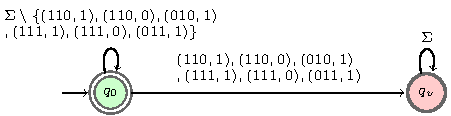
\includegraphics[width=0.5\columnwidth]{fig/sa1-crop2.pdf}
	}
	%	\hspace{0.1em}
	%	\subfloat[Input SA obtained from $\calA_{S_1}$. \label{fig:prop1Inp}]{
		%		\includegraphics[width=0.65\columnwidth]{figures/propA1I.png}
		%	}
	%	\\
	\centering
	\subfloat[SA $\calA_{S_2}$. \label{fig:prop2C}]{
		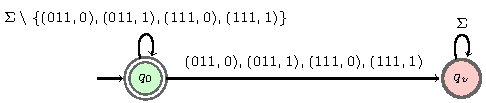
\includegraphics[width=0.5\columnwidth]{fig/sa2-crop2.pdf}
	}
	\hspace{0.1em}
	%	\subfloat[Input SA obtained from $\calA_{S_2}$. \label{fig:prop2Inp}]{
		%		\includegraphics[width=0.65\columnwidth]{figures/propA2I.png}
		%	}
	\caption{Safety automaton for $S_1$ and $S_2$.}
	\label{fig:prop1&2}
\end{figure*}
%%%%%%%%%%%%%%%%%%%%%%%%%%%%%
%%%%%%%%%%%%%%%%%%%%%%%%%%%%%%%%%%%%%%%%%%
\begin{example}[Example policies]
	\label{eg:propC}
	%%%%%%%%%%%%%%%%%%%%%%%%%%%%%%%%%%%%%%%%%%
	%In this section, we will consider the following properties:
	Let $I= \{A,B,C\}$ and $O = \{R\}$.
	Consider the following policies: \textit{$S_1$: ``A and B cannot happen simultaneously, and also B and R cannot happen simultaneously''} and \textit{$S_2$: ``B and C cannot happen simultaneously''}.
	The safety automaton in Figure~\ref{fig:prop1C} and Figure~\ref{fig:prop2C} define policies $S_1$ and $S_2$ respectively.
	%The input safety automaton in Figure~\ref{fig:prop1Inp} and %Figure~\ref{fig:prop2Inp} presents the input SA for $S_1$ and $S_2$ respectively.
\end{example}
%%%%%%%%%%%%%%%%%%%%%%%%%%%%%%%%%%%%%%%%%%%%%
%
%%%%%%%%%%%%%%%%%%%%%%%%%%%%%%%%%%%%%%%%%%%%%
\subsection{Monolithic security enforcement}
%%%%%%%%%%%%%%%%%%%%%%%%%%%%%%%%%%%%%%%%%%%%%
Composing all of the policies first is one way to enforce a collection of policies (taking the product of all the SA).
We can synthesize one enforcer for the resulting policy if the resulting SA is enforceable according to Definition~\ref{def:Enforceability}.


In the monolithic approach, policies (specified as SA) are first combined using intersection (see the Definition~\ref{def:product}, the product of SA), and an enforcer for the resulting policy is synthesized. Specifically, given any two
safety policies $\varphi_1$ and $\varphi_2$, to enforce both these policies, we first compute $\varphi =
\varphi_1 \cap \varphi_2$ (by computing the product of SA for $\varphi_1$ and $\varphi_2$). Then if the resulting SA for $\varphi$ is enforceable as per Definition \ref{def:Enforceability}, we synthesize
an enforcer for $\varphi$ using the approach described in Section \ref{sec:func:def}. 
%For any input word $\sigma$, $E_\varphi(\sigma)$ 
%is sound and transparent with respect to $\varphi_1 \cap \varphi_2$.

%%%%%%%%%%%%%%%%%%%%%%%%%%%%%%%%%%%%%%%%%%%
\begin{figure}[htb]
	\centering
	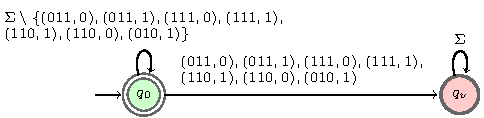
\includegraphics[scale=1]{fig/sa1sa2-crop2.pdf}
	\caption{$\calA_{S_1\cap S_2}$: Product of Automaton $S_1$ and $S_2$}
	\label{fig:prod}
\end{figure}
%%%%%%%%%%%%%%%%%%%%%%%%%%%%%%%%%%%%%%%%%%%

%%%%%%%%%%%%%%%%%%%%%%%%%%%%%%%%%%%%%%%%%%%%% 
\begin{example}[Monolithic approach]
	Consider policies $S_1$ and $S_2$ defined as SAs illustrated in Figure \ref{fig:prop1&2}.
	The SA obtained by taking the product of both these automata is shown in Figure \ref{fig:prod} defining the policy $S_1 \cap S_2$.
	The policy $S_1 \cap S_2$ is enforceable since for every accepting state, there is at least one outgoing transition to an accepting state (See Remark \ref{rem:nonEnf}). Table \ref{table:EgEnf} illustrates behavior of enforcer for policy $\calA_{S_1 \cap S_2}$ when the input-output word $(100,1)\cdot(110,1)\cdot(011,0)$ is processed incrementally.
\end{example}	
%%%%%%%%%%%%%%%%%%%%%%%%%%%%%%%%%%%%%%%%%%%%%

%%%%%%%%%%%%%%%%%%%%%%%%%%%%%%%%%%%
%
\begin{table}[t]
	\centering
	\scalebox{0.8}
	{
		\begin{tabular}{|c|c|c|c|}
			\hline
			$\sigma_I$ & $\sigma_O$ & $\efi(\sigma_I)$ & $\ef(\sigma)=\efo(\efi(\sigma_I), \sigma_O)$ \\
			\hline%
			$\epsilon_I$ & $\epsilon_O$ & $\epsilon_I$ & $(\epsilon_I,\epsilon_O) = \epsilon$\\
			\hline
			$100$ & $1$ & $100$ & $(100,1)$ \\
			\hline
			$100\cdot110$ & $1\cdot1$ & $100\cdot100$ & $(100,1)\cdot(100,1)$ \\
			\hline
			$100\cdot110\cdot011$ & $1\cdot1 \cdot0$ & $100\cdot 100 \cdot 001$ & $(100,1)\cdot(100,1) \cdot(001,0)$ \\
			
			\hline
		\end{tabular}
	}
	\caption{Example illustrating behavior of enforcer for $\calA_{S_1 \cap S_2}$}
	\label{table:EgEnf}
\end{table}
%%%%%%%%%%%%%%%%%%%%%%%%%%%%%%%%


%%%%%%%%%%%%%%%%%%%%%%%%%%%%%%%%%%%%%%%%%%%%% 
\begin{theorem}[Enforceability using the monolithic approach]
	\label{theorem:enforceability-monolithic}
	Consider two policies $\varphi_1$, $\varphi_2$ defined as SA, and $\varphi = \varphi_1 \cap \varphi_2$.
	
	If policy $\varphi_1$  or policy $\varphi_2$ is non-enforceable, then $\varphi_1 \cap \varphi_2$ is non-enforceable.
	%
	
	The proof of Theorem \ref{theorem:enforceability-monolithic} is given in Appendix \ref{proof:enforceability-monolithic}.
	%
	%\SP{We may have to add a brief justification/reasoning for the same.} \Abhinandan{kindly check}
	%This is very much intuitive. If $\varphi_1$  or property $\varphi_2$ is non-enforceable, then there would be no path to an accepting location from a designated location in the SA for any input event. As a result, as per the Definition \ref{def:product}, the product SA will contain a transition that will lead to violating state for any input. Then $\varphi_1 \cap \varphi_2$ is non-enforceable.
\end{theorem}	
%%%%%%%%%%%%%%%%%%%%%%%%%%%%%%%%%%%%%%%%%%%%% 

%%%%%%%%%%%%%%%%%%%%%%%%%%%%%%%%%%%%%%%%%%%%% 
\begin{remark}[Enforceability using the monolithic approach]
	Though policies $\varphi_1$ and $\varphi_2$ are enforceable individually, policy $\varphi_1 \cap \varphi_2$ may not be enforceable, as illustrated in the following example.
\end{remark}
%%%%%%%%%%%%%%%%%%%%%%%%%%%%%%%%%%%%%%%%%%%%% 


%%%%%%%%%%%%%%%%%%%%%%%%%%%%%
\ignore{
	\begin{figure*}
		\begin{centering}
			\scalebox{0.9}{
				\includegraphics[scale=0.1]{fig/nonEnf1.jpg}
			}
			\caption{Policy $\varphi_1\cap \varphi_2$ is non-enforceable. \SP{Abhinandan, you may pl work on this fig and the corresponding explanation of the example!}}
			\label{fig:nonEnf1}
		\end{centering}
	\end{figure*}
} 
%%%%%%%%%%%%%%%%%%%%%%%%%%%%%
%%%%%%%%%%%%%%%%%%%%%%%%%%%%%%%%%%%%%%%%%%%%% 


%%%%%%%%%%%%%%%%%%%%%%%%%%%%%
\begin{figure}%
	\centering
	
	
	\subfloat[SA defining $\varphi_1$- Enforceable \protect\footnotemark]{{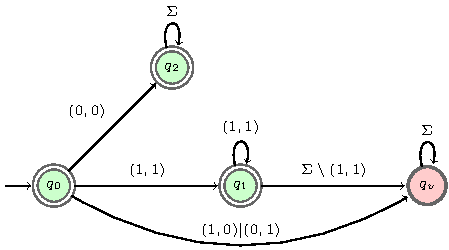
\includegraphics[]{fig/Phi1-crop2.pdf} }}%
	%\qquad
	\vspace{2em}
	\subfloat[SA defining $\varphi_2$- Enforceable \protect\footnotemark ]{{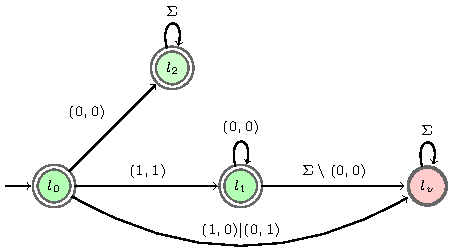
\includegraphics[]{fig/Phi2-crop2.pdf} }}%
	%\qquad
	\vspace{2em}
	\subfloat[SA defining $\varphi_1$ $\cap$ $\varphi_2$]{{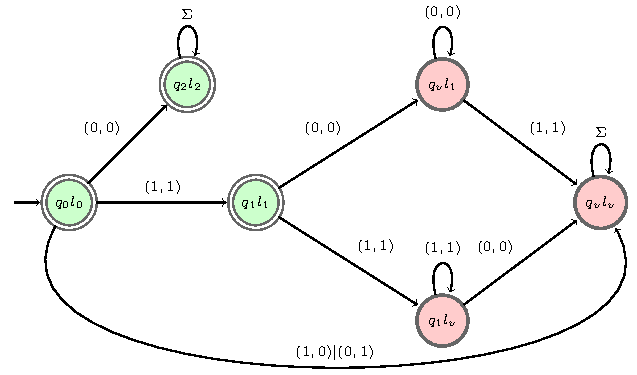
\includegraphics[width=0.9\columnwidth]{fig/Phi1-and-Phi2-cropped.pdf} }}%	
	\caption{Policy $\varphi_1\cap \varphi_2$ is non-enforceable.}
	%	\SP{TO follow a particular color conventions. Reduce space!}
	\label{fig:nonEnf1}
	\vspace{2em}
\end{figure}
\footnotetext[2]{Here, $\Sigma = \{(0,0), (0,1), (1,0), (1,1)\}$. So $\Sigma \setminus (1,1) $ = $\{(0,0), (0,1), (1,0)\}$.}
\footnotetext[3]{Here, $\Sigma = \{(0,0), (0,1), (1,0), (1,1)\}$. So $\Sigma \setminus (0,0) $ = $\{ (0,1), (1,0), (1,1)\}$.}
%%%%%%%%%%%%%%%%%%%%%%%%%%%%%%%%%%%%%%%%%%%%%%%%%%%%%%%%%%%%%%%
\begin{example}[Monolithic approach does not always work]
	Consider the two policies shown in Figure \ref{fig:nonEnf1}. Here $I= \{0,1\}$ and $O = \{ 0,1 \}$. Though they are enforceable individually, the policy that we obtain by taking the product of both the SA $\varphi_1 \cap \varphi_2$ is not enforceable. 
	Suppose that the first event is $(1,1)$, the output of the enforcer will be $(1,1)$, and the state of the product automaton will be updated to $(q_1,l_1)$. When in state $(q_1,l_1)$, whatever may be the input event, it is not possible to correct it (as there will be no path to an accepting state from the state $(q_1,l_1)$ in the product automaton). 
\end{example}	
%%%%%%%%%%%%%%%%%%%%%%%%%%%%%%%%%%%%%%%%%%%%%%%%%%%%%%%%%%%%%%%%%%%%%%%%%%%%%%%%%%%%%%%%%% 
\ignore{
	In \cite{cre2017}, serial and parallel composition approaches were presented. It is shown in \cite{cre2017} that both the compositional approaches work if all the policies are prefix-closed safety policies. However, the enforcement approach considered in \cite{cre2017} is not suitable for reactive systems, since it allows only delaying of events.   }

%In our framework, though prefix-closed safety policies are considered, since the framework allows editing of events, and since enforcers are bi-directional, it is not possible to compose enforcers (as per Definition \ref{def-func-E}) in series or in parallel for the following reasons: 
As discussed in the problem description in the introduction, we focus on how to add a new enforcement layer incrementally to the existing enforcer (e.g., when a new property to be enforced is identified due to a new threat). 
How can an enforcer for the new property be composed with an existing enforcer such that the composed enforcement system, along with the new policy\blue{,} will also continue to enforce all the previously enforced policies is what we explore and study in this work.   



In our framework, since the framework allows editing of events, and since enforcers are bi-directional, it is not possible to compose enforcers (as per Definition \ref{def-func-E}) for the following reasons: 

\squishlist
\item As illustrated in Figure \ref{fig:intro-context}, the enforcer is bi-directional. Firstly, input from the environment is read (and edited/corrected if necessary), which is fed to the program, and the resulting output of the program is later checked (and edited if necessary) by the enforcer before it is forwarded to the environment. This does not allow the enforcers that we have to be composed directly in series. 
\item Moreover, since editing of events is allowed, the edit/correction made by one enforcer may not be compatible w.r.t the other enforcer, where there may be some edit/correction that is suitable for both policies to be enforced.  
\squishend
%%%%%%%%%%%%%%%%%%%%%%%%%%%%%%%%%%%%%%%%%%%%%%%%%%%%%%%%%%%%%%%%%%%%%%%%%%%%%%%%%%%%%%%%%%

Thus we need to revisit the definition of the enforcement function, which will also be suitable for incremental enforcement schemes.
%%%%%%%%%%%%%%%%%%%%%%%%%%%%%%%%%%%%%%%%%%%%%%%
\subsection{Incremental composition of security enforcers} 
\label{sec:serial}
%%%%%%%%%%%%%%%%%%%%%%%%%%%%%%%%%%%%%%%%%%%%%%
Suppose that we rely on the internals of the enforcement function, which composes an input enforcement function and an output enforcement function, then we can consider:
%in serial composition approach,
\squishlist
\item composing all the input enforcement functions in series, where the (corrected) input that is released by the last function is fed to the program.
\item similarly, the output enforcement functions can also be combined in series\blue{,} and the corrected output released by the last function can be emitted to the environment. 
\squishend

The incremental scheme by composing enforcers in series is shown in Figure \ref{fig:serialComp1}.

%%%%%
%\SP{Abhinandan, may pl add a figure illustrating the scheme/approach.}
%%%%%%%%%%%%%%%%%%%%%%%%%%%%%%%%%%%%
Given two policies $\varphi_1$ and $\varphi_2$ (where $\varphi_{1I}$ and $\varphi_{2I}$ are their corresponding input policies)\blue{,} we can synthesize input and output enforcement functions for each of these policies $\efi{\varphi_1}$,  $\efi{\varphi_2}$, $\efo{\varphi_1}$, and $\efo{\varphi_2}$, 
and then compose all the input enforcers and all the output enforcers. The composed input enforcer can be then combined with the composed output enforcer (see Figure \ref{fig:serialComp1}).

%%%%%%%%%%%%%%%%%%%%%%%%%%%%%%%%%%%%%%%%%%%%%%%
\begin{SingleColFigure}
	\centering
	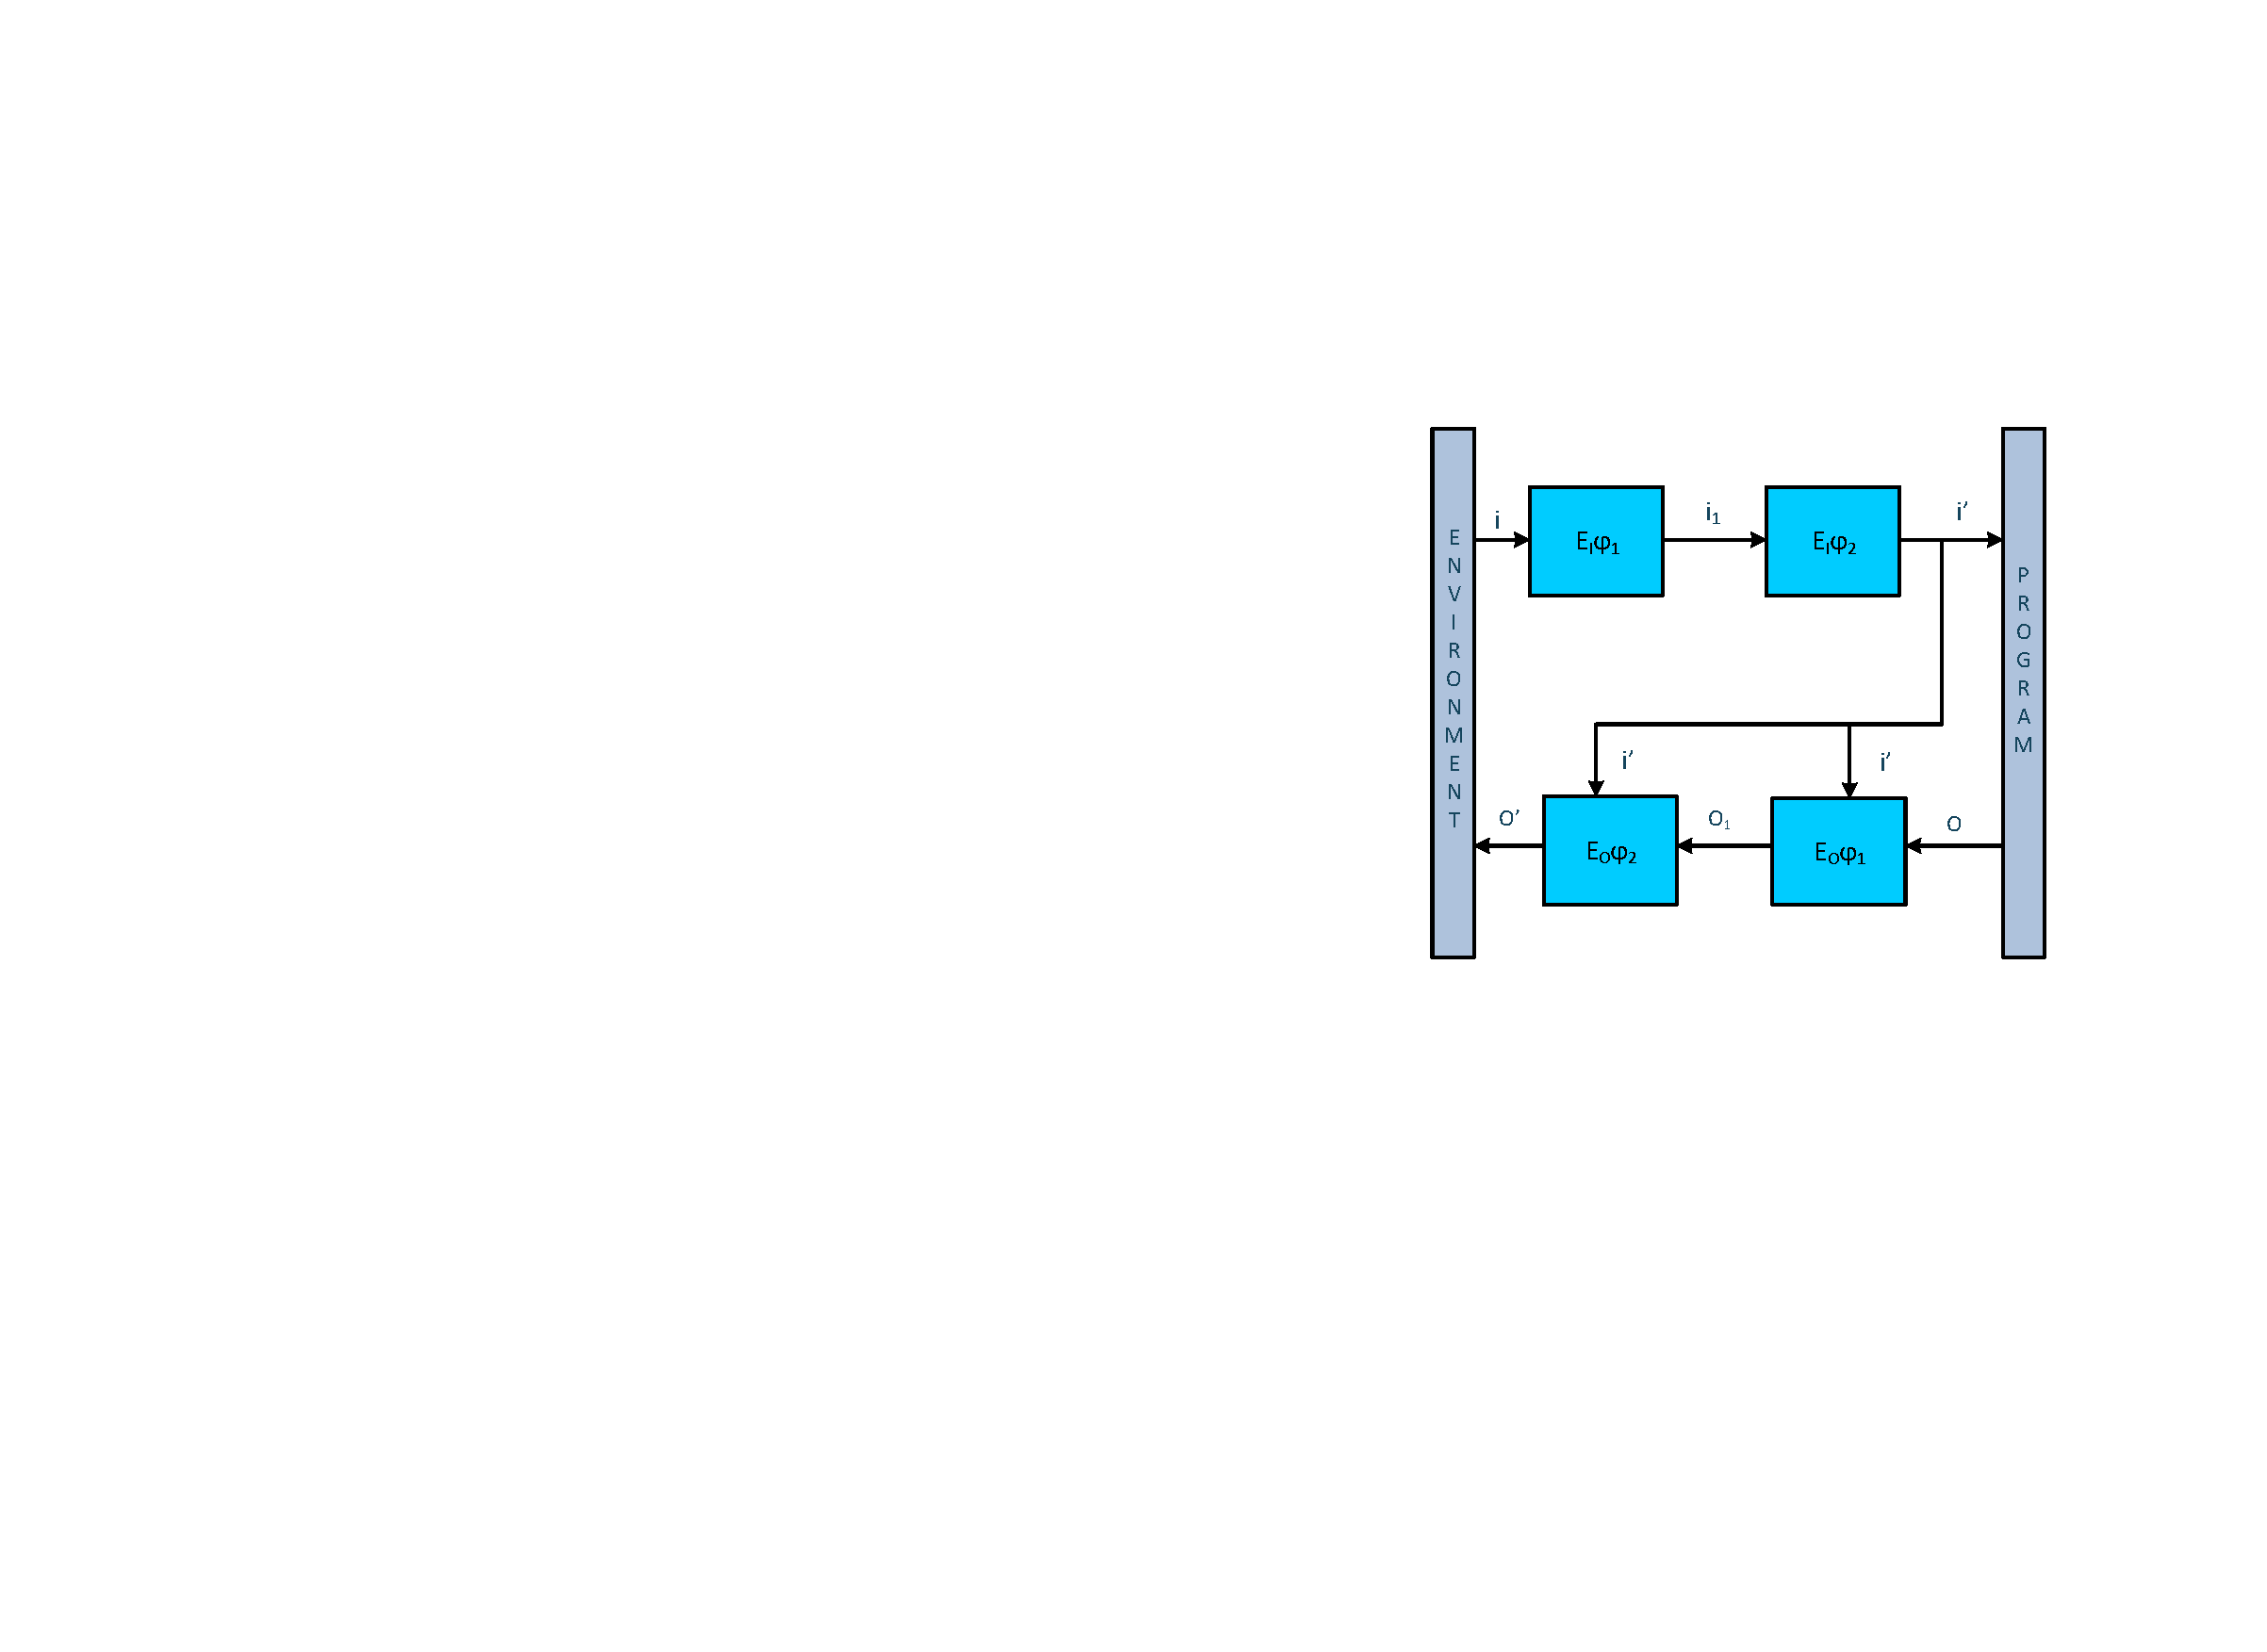
\includegraphics[width=\columnwidth]{fig/serial composition-ColourDiagram-cropped2.pdf}
	\captionof{figure}{Incremental enforcement via serial composition}
	%\SP{Abhinandan, may pl add a figure !}
	
	\label{fig:serialComp1}
\end{SingleColFigure}
%%%%%%%%%%%%%%%%%%%%%%%%%%%%%%%%%%%%%%%%%%

We denote this type of incremental composition of enforcers in series as  $\e{\varphi_1} \serial \e{\varphi_2}$.
% In this type of serial composition, the output of $\e{\varphi_1}$ is fed as input to $\e{\varphi_2}$. As a result we obtain a new EM, denoted $\e{\varphi_1} \serial \e{\varphi_2}$.
In this section we investigate whether $\e{\varphi_1} \serial \e{\varphi_2}$
generally enforces $\varphi_1\cap\varphi_2$.
We are also interested to see whether the final output that we obtain using the incremental composition approach is equal to the output we would obtain using the monolithic approach.
%%%%%%%%%%%%%%%%%%%%%%%%%%%%%%%%%%%%%

Let us now formally define incremental composition in series of two enforcers.

%%%%%%%%%%%%%%%%%%%%%%%%%%%%%%%%%%
\begin{definition}[Incremental enforcement via serial composition]
	\label{def:serialComp}
	Let $\efi{\varphi_1}: \Sigma_I^* \rightarrow \Sigma_I^*$ (resp. $\efi{\varphi_2}: \Sigma_I^* \rightarrow \Sigma_I^*$) be the input enforcement function for policy $\varphi_{1I}  \subseteq \Sigma_I^*$ (resp. $\varphi_{2I}$), and 
	let 
	$\efo{\varphi_1}: \Sigma_I^* \times \Sigma_O^* \rightarrow (\Sigma_I \times \Sigma_O)^*$ (resp. $\efo{\varphi_2}$) be the output enforcement function for policy $\varphi_1  \subseteq \Sigma^*$ (resp. $\varphi_2$). 
	Their serial composition is a new enforcer $\e{\varphi_1} \serial \e{\varphi_2}: \Sigma^* \rightarrow \Sigma^*$ defined as follows:
	\[
	\forall \sigma\in\Sigma^*,
	(\e{\varphi_1} \serial \e{\varphi_2})(\sigma)
	= \efo{\varphi_2}(\sigma'_I, \sigma'_O).
	\]
	with $\sigma'_I = \efi{\varphi_2}(\efi{\varphi_1}({\sigma_I}))$, and $\sigma'_O = \efo{\varphi_1}(\sigma'_I, \sigma_O)$.
\end{definition}
%%%%%%%%%%%%%%%%%%%%%%%%%%%%%%%%%%
%%%%%%%%%%%%%%%%%%%%%%%%%%%%%%%%%%
%\SP{We may add a brief 1-2 lines expl of the def.}\Abhinandan{kindly check.}
As per the composition Definition \ref{def:serialComp}, the output of the serial composition of the enforcers is the output emitted from the output enforcer \efo{$\varphi_2$}. The input emitted from the input enforcer \efi{$\varphi_2$} is considered as the final corrected input. The output enforcer \efo{$\varphi_1$} is invoked with the corrected input $\sigma'_I$ from the serially composed input enforcers and the output $\sigma_O$ of the reactive system. The corrected output of the enforcer is input to the output enforcer \efo{$\varphi_2$}, which finally emits the output to the environment.   
%%%%%%%%%%%%%%%%%%%%%%%%%%%%%%%%%%%%%

\begin{table*}
	%\vspace{-1em}
	\centering
	\begin{tabular}{|c|c|c|c|c|c|}
		\hline
		$\sigma_I$ & $\sigma_O$ & $\sigma'_I = \efi{S1}(\sigma_I)$ & $\sigma^{''}_I = \efi{S2}(\sigma'_I)$ & $ \sigma'_O = \efo{S1}(\sigma^{''}_I, \sigma_O)$ & $\efo{S2}(\sigma^{''}_I, \sigma'_O)$ \\
		\hline
		$100$ & $1$ & $100$ & $100$ &  $(100,1)$ & $(100,1)$ \\
		\hline
		$100 \cdot 110$ & $1 \cdot 1 $ & $100 \cdot 011$ & $100 \cdot 110$ &  $(100,1) \cdot ??$ & -- \\
		
		\hline
	\end{tabular}
	\caption{Serial composition using Definition \ref{def:serialComp}}
	\label{tableEgSerialDef}
\end{table*}
%%%%%%%%%%%%%%%%%%%%%%%%%%%%%%%%%%%%%%%%%%%%%%%%%%%%%%%%%%%%%%%%%%%%%%%%%
\begin{figure*}
	%
	\centering
	\subfloat[SA $\calA_{S_1}$. \label{fig:prop1C}]{
		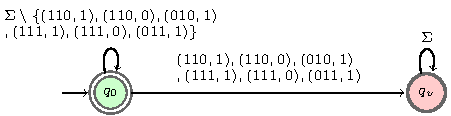
\includegraphics[width=0.5\columnwidth]{fig/sa1-crop2.pdf}
	}
	%	\hspace{0.1em}
	%	\subfloat[Input SA obtained from $\calA_{S_1}$. \label{fig:prop1Inp}]{
		%		\includegraphics[width=0.65\columnwidth]{figures/propA1I.png}
		%	}
	%	\\
	\centering
	\subfloat[SA $\calA_{S_2}$. \label{fig:prop2C}]{
		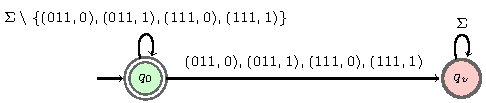
\includegraphics[width=0.5\columnwidth]{fig/sa2-crop2.pdf}
	}
	\hspace{0.1em}
	%	\subfloat[Input SA obtained from $\calA_{S_2}$. \label{fig:prop2Inp}]{
		%		\includegraphics[width=0.65\columnwidth]{figures/propA2I.png}
		%	}
	\caption{Safety automaton for $S_1$ and $S_2$.}
	\label{fig:prop1&2-duplicate}
\end{figure*}
%%%%%%%%%%%%%%%%%%%%%%%%%%%%%%%%%%%%%%%%%%%%%%%%%%%%%%%%%%%%%%%%%%%%%%%%%%%%%%%%%%%%%%%%%%%%%%%%%%%%
\begin{remark}
	
	Definition \ref{def:serialComp} is formulated in order to support incrementally adding a new enforcement layer. Suppose that we only have the input and output enforcement functions w.r.t policy $\varphi_1$ and a new policy to be enforced $\varphi_2$ is given. 
	We can obtain enforcement functions for $\varphi_2$ individually and compose with the existing enforcement functions as per Definition \ref{def:serialComp}.
	
\end{remark}
%%%%%%%%%%%%%%%%%%%%%%%%%%%%%%%%%%%%%

\emph{Note that serial composition of enforcers as per Definition \ref{def:serialComp} does not always work. 
	That is, though given two policies $\varphi_1$, $\varphi_2$ and also $\varphi_1 \cap \varphi_2$ are all enforceable, the serial composition of enforcers of $\varphi_1$ and $\varphi_2$ as per the above definition may not work. The final output obtained may not satisfy $\varphi_1 \cap \varphi_2$. Moreover, there may also be situations where other constraints\blue{,} such as instantaneity\blue{,} may be violated.} Let us consider input enforcement to understand this (similar reasoning also applies for output enforcement). As per the serial composition definition (Def. \ref{def:serialComp}), the input emitted from the input enforcer \efi{$\varphi_2$} is considered as the final corrected input, but the final input selected by the function $\efi{\varphi_2}$  may violate the policy monitored by the input enforcer $\efi{\varphi_1}$.     

Let us consider the following example to understand this further.


\begin{example}[{Serial composition as per Definition \ref{def:serialComp} does not always work}]
	Let us again consider policies $S_1$ and $S_2$ illustrated in Figure \ref{fig:prop1&2}, presented again in Figure \ref{fig:prop1&2-duplicate}. 
	Both policies $S_1$ and $S_2$ are enforceable individually. The policy $S_1 \cap S_2$ is also enforceable. 
	However, when we compose input and output enforcers for these policies in series as per Definition \ref{def:serialComp}, the final output obtained may not satisfy policy $S_1 \cap S_2$. 
	Also, there may be situations where constraints such as instantaneity may be violated. 
	For example\blue{,} consider the word $(100,1) \cdot (110,1) \cdot (011,0)$ to be processed incrementally.   
	In the first step, $(100,1)$ satisfies both policies and thus will be emitted as it is.
	In the second step, let us consider that the altered input produced by the second input enforcement function is $110$. 
	When $110$ is fed as input to the output enforcement function of policy $S_1$, there is no possible output event that it can release to satisfy policy $S_1$. The incremental processing of the considered word is shown in Table \ref{tableEgSerialDef}.	
\end{example}

%%%%%%%%%%%%%%%%%%%%%%%%%%%%%%%%%%
%%%%%%%%%%%%%%%%%%%%%%%%%%%%%%%%%%%
\ignore{
	\begin{table*}
		\vspace{-1em}
		\centering
		\begin{tabular}{|c|c|c|c|c|c|}
			\hline
			$\sigma_I$ & $\sigma_O$ & $\sigma'_I = \efi{S1}(\sigma_I)$ & $\sigma^{''}_I = \efi{S2}(\sigma'_I)$ & $ \sigma'_O = \efo{S1}(\sigma^{''}_I, \sigma_O)$ & $\efo{S2}(\sigma^{''}_I, \sigma'_O)$ \\
			\hline
			$100$ & $1$ & $100$ & $100$ &  $(100,1)$ & $(100,1)$ \\
			\hline
			$100 \cdot 110$ & $1 \cdot 1 $ & $100 \cdot 011$ & $100 \cdot 110$ &  $(100,1) \cdot ??$ & -- \\
			
			\hline
		\end{tabular}
		\caption{Serial composition using definition \ref{def:serialComp}}
		\label{tableEgSerialDef}
	\end{table*}
}
%%%%%%%%%%%%%%%%%%%%%%%%%%%%%%%%
%%%%%%%%%%%%%%%%%%%%%%%%%%%%%%%%
%
%%%%%%%%%%%%%%%%%%%%%%%%%%%%%%%%%%%%%%%%%%%%%%%%
%\subsection{Parallel composition of enforcers} 
%\label{sec:parallel}
%%%%%%%%%%%%%%%%%%%%%%%%%%%%%%%%%%%%%%%%%%%%%%%
%
%
%Parallel composition of enforcers generally does not work because enforcers should react instantaneously and they are allowed to edit events.
%%%%%%%%%%%%%%%%%%%%%%%%%%%%%%%%%%%%%%%%%%%%%%%%
%\begin{SingleColFigure}
%	\centering
%	\includegraphics[width=0.9\columnwidth]{figures/parallel1.jpeg}
%	\captionof{figure}{Parallel Composition \SP{Abhinandan, may pl add a figure !}}
%	\label{fig:parallelComp1}
%\end{SingleColFigure}
%%%%%%%%%%%%%%%%%%%%%%%%%%%%%%%%%%%%%%%%%%%%%%%%
%%%%%%%%%%%%%%%%%%%%%%%%%%%%%%%%%%%%%%%%%%%%%%%%
%\begin{SingleColFigure}
%	\centering
%	\includegraphics[width=0.9\columnwidth]{fig/parallel-composition-crop.pdf}
%	\captionof{figure}{Parallel Composition}
%	\label{fig:parallelComp1}
%\end{SingleColFigure}
%%%%%%%%%%%%%%%%%%%%%%%%%%%%%%%%%%%%%%%%%%%%%%%%
%\vspace{0.5em}
%Let us consider parallel composition of the input enforcers. At the beginning of each tick, each input enforcer is fed with the same input (input observed from the environment), each of them emits a corrected input according to its property. There should be some mechanism for selecting one corrected input from the corrected inputs emitted by all the enforcers. 
%
%Let us consider two properties $\varphi_1$ and $\varphi2$ (where $\varphi_{1I}$ and $\varphi_{2I}$ are their corresponding input properties). we can synthesize input and output enforcement functions for each of these properties $\efi{\varphi_1}$,  $\efi{\varphi_2}$, $\efo{\varphi_1}$, and $\efo{\varphi_2}$.
% 
%As illustrated in Figure \ref{fig:parallelComp1}, we can consider composing the input enforcers in parallel, where input from the environment $i$ is fed as input to both the input enforcers in parallel. Each input enforcer emits transformed input $i_1$ (resp. $i_2$), which are fed as input to the $Merge_I$ function, which picks one among them randomly ($i'$) and emits it to the program. 
%
%Similarly, the output from the program $o$ can be fed in parallel to both the output enforcers  $\efo{\varphi_1}$, and $\efo{\varphi_2}$, Each output enforcer produces transformed output $o_1$ (resp. $o_2$). which are fed as input to the $Merge_O$ function, which picks one among them randomly ($o'$) and emits it to the environment. 
%   
%
%%%%%%%%%%%%%%%%%%%%%%%%%%%%%%%%%%%%%%%%%%%%%%%%%%%%%%%%%%%%%%%%%
%%%%%%%%%%%%%%%%%
%\begin{definition}[Parallel composition of enforcement monitors]
%	\label{def:parallelComp}
%Let $\efi{\varphi_1}: \Sigma_I^* \rightarrow \Sigma_I^*$ (resp. $\efi{\varphi_2}: \Sigma_I^* \rightarrow \Sigma_I^*$) be the input enforcement function for property $\varphi_{1I}  \subseteq \Sigma_I^*$ (resp. $\varphi_{2I}$), and 
%let 
%$\efo{\varphi_1}: \Sigma_I^* \times \Sigma_O^* \rightarrow (\Sigma_I \times \Sigma_O)^*$ (resp. $\efo{\varphi_2}$) be the output enforcement function for property $\varphi_1  \subseteq \Sigma^*$ (resp. $\varphi_2$). 
%
%Their parallel composition is a new enforcer $\e{\varphi_1} || \e{\varphi_2}: \Sigma^* \rightarrow \Sigma^*$ defined as follows:
%
%	$
%	\forall \sigma\in\Sigma^*, (\e{\varphi_1}|| \e{\varphi_2})(\sigma) = Merge_O(\efo{\varphi_1}(\sigma'_I, \sigma_O), \efo{\varphi_2}(\sigma'_I, \sigma_O)).
%	$
%	
%	with $\sigma'_I = Merge_I(\efi{\varphi_1}(\sigma_I), \efi{\varphi_2}(\sigma_I))$.
%\end{definition}
%%%%%%%%%%%%%%%%%%%%%%%%%%%%%%%%%%%%%%%%%%%%%%%%%%%%%%%%%%%%%%%%
%
%
%%There is no such possible mechanism, as selecting any input from the corrected inputs emitted the input enforcers may violate the property monitored by the other input enforcers. 
%
%
%Note that parallel composition of enforcers does not always work. That is, though given two properties $\varphi_1$, $\varphi_2$ and also $\varphi_1 \cap \varphi_2$ are all enforceable, parallel composition of enforcers of $\varphi_1$ and $\varphi_2$ as per the above definition may not work. The final output obtained may not satisfy $\varphi_1 \cap \varphi_2$. Moreover, there may be also situations where other constraints such as instantainety may be violated.
%Let us consider input enforcement to understand this (similar reasoning also applies for output enforcement). As per the parallel composition definition (Def. \ref{def:parallelComp}), any input from the corrected inputs emitted the input enforcers can be selected as the final corrected input. The final input selected by the $Merge_I$ function may violate the property monitored by the some of the input enforcers.     
%
%Let us consider the following example to understand this further.
%
%%%%%%%%%%%%%%%%%%%%%%%%%%%%%%%%%%%
%%%%%%%%%%%%%%%%%%%%%%%%%%%%%%%%%%%%
%%
%\begin{table*}[]
%	\centering
%	\begin{tabular}{|c|c|c|c|c|c|c|c|}
	%		\hline
	%		$\sigma_I$ & $\sigma_O$ & $\efi{S1}(\sigma_I)$ & $\efi{S2}(\sigma_I)$ & $\sigma'_I= Merge_I()$ & $\efo{S1}(\sigma'_I, \sigma_O)$&$\efo{S2}(\sigma'_I, \sigma_O)$&$Merge_O()$\\
	%		\hline
	%		$100$ & $1$ & $100$ & $100$ & $100$& $(100,1)$ & $(100,1)$ & $(100,1)$ \\
	%		\hline
	%		$100 \cdot 110$ & $1 \cdot 1 $ & $100 \cdot 011$ & $100 \cdot 110$& $100 \cdot 110$ & $(100,1) \cdot ?? $ & -- & -- \\
	%%		
	%		\hline
	%	\end{tabular}
%	\caption{Parallel composition}
%	\label{tableEgParallelDef}
%\end{table*}
%%%%%%%%%%%%%%%%%%%%%%%%%%%%%%%%%
%%%%%%%%%%%%%%%%%%%%%%%%%%%%%%%%%
%\begin{example}[Parallel composition does not work]
%
%Let us again consider properties $S_1$ and $S_2$ illustrated in Figure \ref{fig:prop1&2}. 
%Both properties $S_1$ and $S_2$ are enforceable individually. The property $S_1 \cap S_2$ is also enforceable. 
%However, when we compose input and output enforcers for these properties in parallel as per Definition \ref{def:parallelComp}, the final output obtained may not satisfy property $S_1 \cap S_2$. %Also, there may be situations where constraints such as instantainety may be violated.
% For example consider the word $(100,1) \cdot (110,1) \cdot (011,0)$ to be processed incrementally.   
%In the second step, when the input $110$ is fed to both the input enforcement function parallely, the two enforcers may emit $011$ and $110$, respectively satisfying respective property. As per parallel composition mechanism, any one of the corrected inputs may be emmitted as the final output, say $110$ in this case. When the input given to the output enforcement function of property $S_1$ is $110$, there is no possible input-output event that it can release as output continuing to satisfy property $S_1$. The incremental processing of the considered word is shown in Table \ref{tableEgParallelDef}.	
%
%\SP{Abhinandan, may pl check, explain the example!}	
%\end{example}

%\blue{We thus revisit the incremental security enforcement scheme in the next section.   
	%}

In this section, we have seen that the enforcement function in Definition \ref{def-func-E}  is not always suitable for the incremental security enforcement by composing enforcers in series, also when we consider first composing all the input enforcement functions, followed by the composition of the output enforcement functions (Definition \ref{def:serialComp}).



We thus revisit the incremental security enforcement scheme in the next section, to propose an incremental scheme that can tackle all the enforceable properties.


%%%%%%%%%%%%%%%%%%%%%%%%%%%%%%%%%%%%%%%%%%%%%%%%%%%%%%%%
%%%%%%%%%%%%%%%%%%%%%%%%%%%%%%%%%%%%%%%%%%%%%%%%%%%%%%%%
\section{Revisiting Incremental Security Enforcement  Scheme}
\label{sec:new:def}
%(its corresponding enforcement algorithm given in Definition \ref{def:Enforceability})
In this section we propose an incremental composition scheme. First, we define the following Select functions and later present how the compositional scheme can be defined using the Select functions. 
%We later define serial and parallel composition and show that for any given set of properties, that are enforceable using the monolithic approach, they are also enforceable using both serial and parallel composition schemes.

%%%%%%%%%%%%%%%%%%%%%%%%%%%%%%%%%%%%%%%%%%%%%%%%%%%%%%%%
%%%%%%%%%%%%%%%%%%%%%%%%%%%%%%%%%%%%%%%%%%%%%%%%%%%%%%%% 
%
%%%%%%%%%%%%%%%%%%%%%%%%%%%%%%%%%%%%%%%%%%%%%%%%%%%%%%%%
\subsection{Select Functions}
\label{sec:new:edit}
%%%%%%%%%%%%%%%%%%%%%%%%%%%%%%%%%%%%%%%%%%%%%%%%%%%%%%%%
%\red{Briefly discuss why we need to redefine edit functions in the following manner. Set of all possible inputs fed to the first edit/select function.}

%\SP{Abhinandan, pl check the notes/presentation and see to revise these definitions !}
%

%\SP{We may add simple examples to illustrate these select functions.}\Abhinandan{kindly check.}
\squishlist
\item {{\boldmath$\selectI_{\varphi_{I}}(\sigma_I, X)$}}: Given an input word $\sigma_I\in\Sigma_I^*$, and a set of input events $X \subseteq \Sigma_I$, $\selectI_{\varphi_{I}}(\sigma_I, X)$ is the set of input events $x$ that belong to set $X$ such that the word obtained by extending $\sigma_I$ with $x$ satisfies policy $\varphi_I$. Formally,
\[\selectI_{\varphi_{I}}(\sigma_I, X) = \{ x\in X: \sigma_I \cdot x \models \varphi_I \}.\]
%
Considering the SA $\calA_{\varphi_I}=(Q, q_0, q_v, \Sigma_I, \rightarrow_I)$,
the set of events in $X$ that allow to reach a state in $Q\setminus \{q_v\}$ from a state $q\in Q\setminus \{q_v\}$ is defined as:
\[\selectI_{\calA_{\varphi_I}}(q,X) = \{x\in X: q \xrightarrow{x}_I q' \wedge q' \neq q_v \}. \]
%
For example, let us consider the input automaton corresponding to policy $P$ in Figure \ref{fig:prop1Inp}.
Initially, when $\sigma_I = \epsilon$ we have $X = \{00,01,10,11\}$, and $\selectI_{P}(\epsilon, X)= \{00,01,10\}$.
%
If we consider $\sigma_I = 00 \cdot 01 \cdot 01$, and  $X = \{00,01,10\}$, we have $\selectI_{P}(00 \cdot 01, X)= \{00,01,10\}$.

Also, $q_0 \xrightarrow{00\cdot01}_I q_0$, and $\selectI_{P}(q_0, \{00,01,10\}) = \{00,01,10\}$.


%For example, consider the the property $S_1$ illustrated in Figure \ref{fig:prop1&2} by ignoring outputs. In this case, the set of valid inputs, $X$= $(100,101,010,001,011)$. Let $\sigma= (100,1)\cdot(110,1)$, and thus $\sigma_I= 100\cdot110$. Then, $\selectI_{S1}(\sigma_I, X)=\{100,101,010,001,011\}$.

%$\editI(\sigma_I) = \Sigma_I\setminus\{11\}$.


%Also, $q_0 \xrightarrow{100\cdot110}_I q_0$, and $\selectI_{S1}(q_0,X) = \{100,101,010,001,011\}$.



%If $\editIaut(q)$ is non-empty, then $\randEditIaut(q)$ returns an element (chosen randomly) from $\editIaut(q)$, and is undefined if $\editIaut(q)$ is empty.
%
\item {\boldmath$\selectO_\varphi(\sigma, x, Y)$}:~~Given an input-output word $\sigma\in\Sigma^*$, an input event $x\in\Sigma_I$, and a set of output events $Y \subseteq \Sigma_O$, $\selectO_\varphi(\sigma, x, Y)$ is the set of output events $y$ in $Y$ s.t. the input-output word obtained by extending $\sigma$ with $(x,y)$ satisfies policy $\varphi$. Formally,
\[\selectO_\varphi(\sigma,x, Y) = \{y \in Y: \sigma \cdot (x,y) \models \varphi \}.\]
%
Considering the automaton $\calA_{\varphi}=(Q, q_0, q_v, \Sigma, \rightarrow)$ defining policy $\varphi$, and an input event $x\in\Sigma_I$,
the set of output events $y$ in $Y$ that allow to reach a state in $Q\setminus \{q_v\}$ from a state $q\in Q\setminus \{q_v\}$ with $(x,y)$ is defined as:
\[\selectO_{\calA_{\varphi}}(q,x, Y) = \{y \in Y: q \xrightarrow{(x,y)} q' \wedge q' \neq q_v \}. \]
%
\squishend

For example, consider policy $P$ illustrated in Figure \ref{fig:prop1}. We have $\selectO_{P}(q_0, 01, \{0,1\}) = \{0\}$.

%For example, consider property $S_1$ defined by the automaton in Figure~\ref{fig:prop1}.
%We have $\editOaut(q_0, 01) = \{0\}$.
%
%If $\editOaut(q,x)$ is non-empty, then $\randEditOaut(q, x)$ returns an element (chosen randomly) from $\editOaut(q,x)$, and is undefined if $\editOaut(q,x)$ is empty.




{\boldmath$\minEdit(x, X')$ (resp. \boldmath$\minEdit(y, Y')$)}: Consider $X'$ (resp. $Y'$) as a set of input (resp. output) events acceptable to all policies $\varphi$, and $x$ (resp. $y$) as the original input (resp. output). $\minEdit(x, X')$ (resp. $\minEdit(y, Y')$) non-deterministically selects an edit $x' \in X'$ (resp. $y' \in Y'$) such that it is of minimum deviation from the original input event $x$ (resp. output event $y$).
%%%%%%%%%%%%%%%%%%%%%%%%%%%%%%%%

\begin{table*}
	\vspace{-1em}
	\centering
	\resizebox{.9\textwidth}{!}{% <------ Don't forget this %
		\begin{tabular}{|c|c|c|c|c|c|}
			\hline
			$\sigma_I$ & $\sigma_O$ & $X_1 = \selectI_{S1}(\sigma'_I,\Sigma_I)$ & $X' = \selectI_{S2}(\sigma'_I,X_1)$ & $x'= MinD(x,X')$ & $\sigma'_I$  \\
			\hline
			$100$ & $1$ & $\selectI_{S1}(\epsilon_I,\Sigma_I)=\{100,101,010,001,011\}$ & $\selectI_{S2}(\epsilon_I,X_1)=\{100,101,010,001\}$ & $MinD(100,\{100,101,010,001\})=100$ &  $100 $  \\
			\hline
			$100 \cdot 110$ & $1 \cdot 1 $ & $\selectI_{S1}(100,\Sigma_I)=\{100,101,010,001,011\}$ & $\selectI_{S2}(100,X_1)=\{100,101,010,001\}$ & $MinD(110,\{100,101,010,001\})=100$ & $100 \cdot 100 $  \\
			
			\hline
			$100 \cdot 110 \cdot 011$ & $1 \cdot 1 \cdot 0 $ & $\selectI_{S1}(100.100,\Sigma_I)=\{100,101,010,001,011\}$  & $\selectI_{S2}(100\cdot100,X_1)=\{100,101,010,001\}$ & $ MinD(011,\{100,101,010,001\})=001$ &  $100 \cdot 100 \cdot 001$ \\
			
			\hline
		\end{tabular}
	}
	\caption{Serial composition scheme using Select()-input enforcement}
	\label{table:EgSerialDef21}
	
\end{table*}
%%%%%%%%%%%%%%%%%%%%%%%%%%%%%%%%
\begin{table*}
	\vspace{-1em}
	\centering
	\resizebox{.9\textwidth}{!}{% <------ Don't forget this %
		\begin{tabular}{|c|c|c|c|}
			\hline
			$Y' = \selectO_{S1}(\sigma',x',\Sigma_O)$ & $Y''=\selectO_{S2}(\sigma',x',Y')$ & $MinD(y,Y'')$ & $\sigma'$\\
			\hline
			$\selectO_{S1}(\epsilon,100,\Sigma_O)=\{0,1\}$ & $\selectO_{S2}(\epsilon,100,Y')=\{0,1\}$ & $MinD(1,\{0,1\})=1$ & $(100,1)$ \\
			\hline
			$\selectO_{S1}((100,1),100,\Sigma_O)=\{0,1\}$ & $\selectO_{S2}((100,1),100,Y')=\{0,1\}$ & $MinD(1,\{0,1\})=1$ & $(100,1) \cdot (100,1)$ \\
			
			\hline
			$\selectO_{S1}((100,1)\cdot (100,1),001,\Sigma_O)=\{0,1\}$ & $\selectO_{S2}((100,1)\cdot (100,1),001,Y')=\{0,1\}$ & $MinD(0,\{0,1\})=0$ & $(100,1) \cdot (100,1) \cdot (001,0)$\\
			
			\hline
		\end{tabular}
	}
	\caption{Serial composition scheme using Select()-output enforcement}
	\label{table:EgSerialDef22}
	
\end{table*}

%%%%%%%%%%%%%%%%%%%%%%%%%%%%%%%%%%%%%%%%%%%%%%%%%%

%%%%%%%%%%%%%%%%%%%%%%%%%%%%%%%%%%%%%%%%%%%%%%%%%%%%%%%%
\subsection{Incremental Enforcement Scheme using Select Functions}
\label{sec:framework:serial}
%%%%%%%%%%%%%%%%%%%%%%%%%%%%%%%%%%%%%%%%%%%%%%%%%%%%%%%%
%\SP{Abhinandan, pl check the notes/definitions discussed, also added in the repo in the Notes directory. May pl add a draft of the section including the figures, illustrative example etc.}

%%%%%%%%%%%%%%%%%%%%%%%%%%%%%%%%%%%%%%%%%%%%%%%
\begin{SingleColFigure}
	\centering
	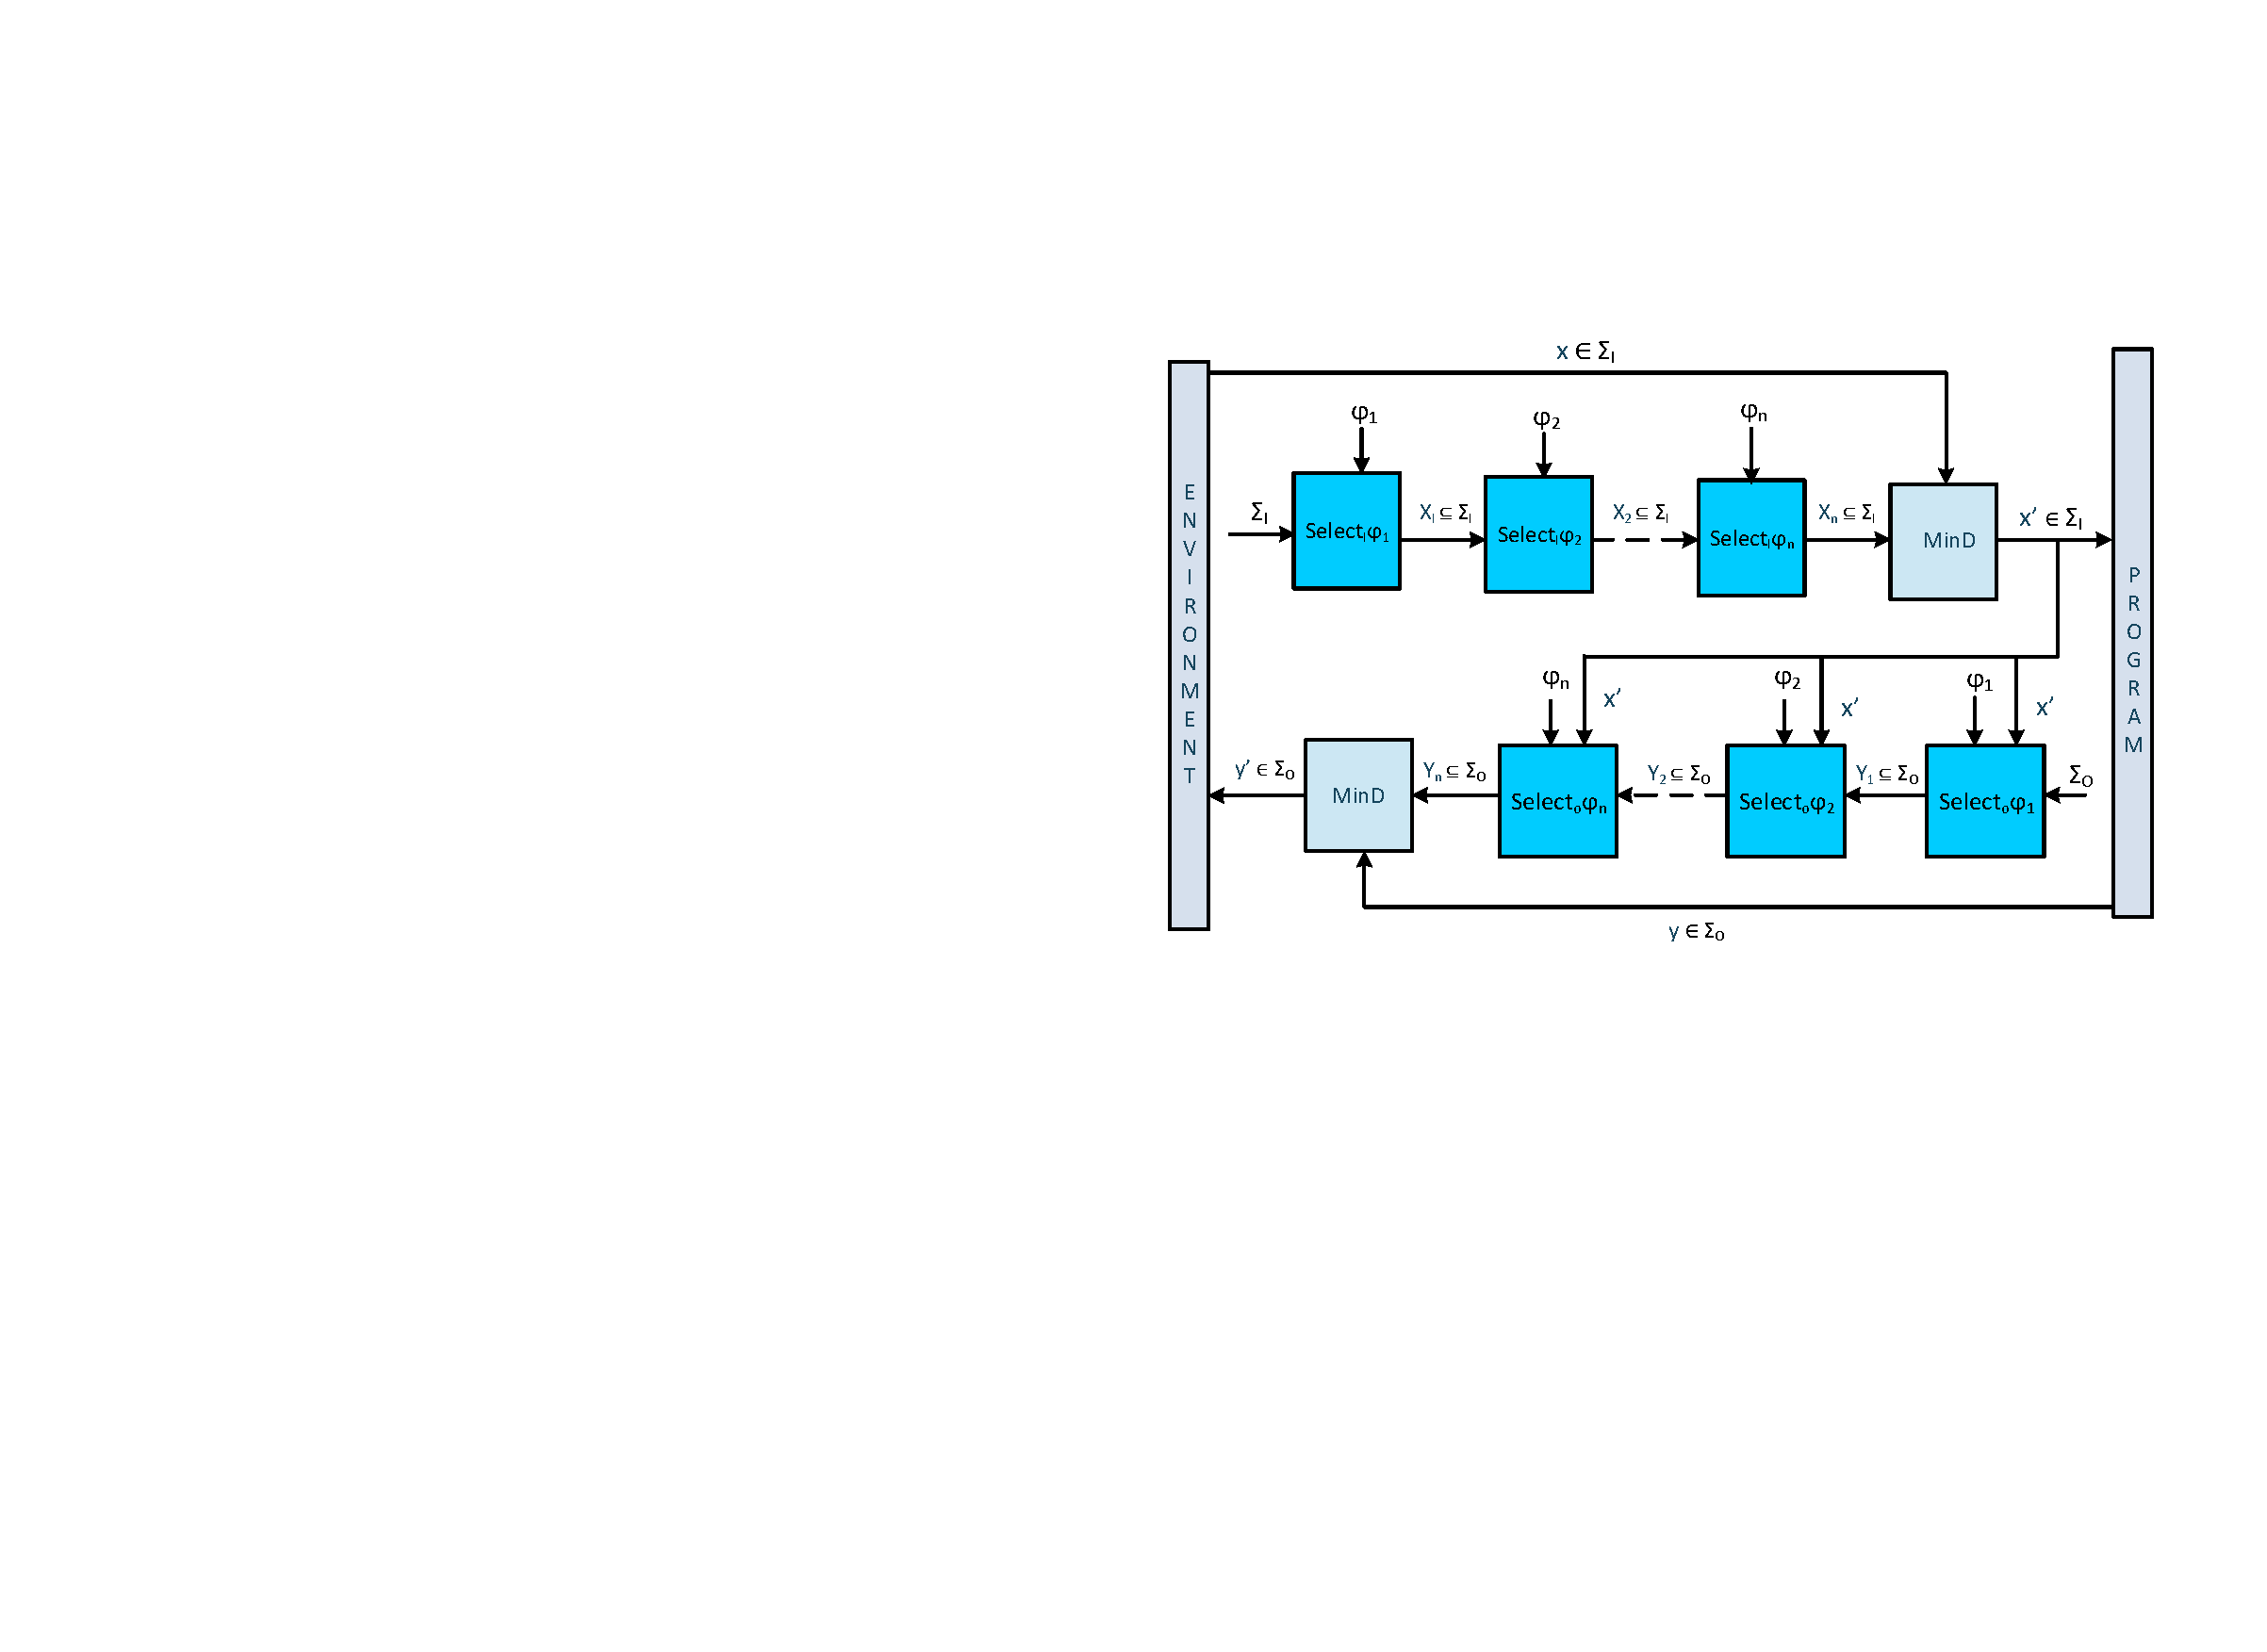
\includegraphics[width=1.1\columnwidth]{fig/serial-composition2-ColourDiagram-cropped5.pdf}
	\captionof{figure}{Incremental Enforcement via Serial Composition using Select functions}
	\label{fig:serialComp2}
\end{SingleColFigure}
%%%%%%%%%%%%%%%%%%%%%%%%%%%%%%%%%%%%%%%%%%%%%%%%%%%%%%%%%%%%%%%%

In serial composition using Select, the input enforcer $\efi$ is implemented by the serial composition of $\selectI()$ followed by MinD(). The input set $\Sigma_I$ is fed to $\selectI()$ in serial to pre-compute a valid input set satisfying all policies. As shown in Figure \ref{def:serialComp2}, $\selectI_{\varphi_{1}}$ produces input set $X_1$ according to policy $\varphi_{1I}$ from input $\Sigma_I$. Similarly, $\selectI_{\varphi_{2}}$ outputs set $X_2$ w.r.t policy $\varphi_{2I}$ from input $X_1$ and so on. The final input set  obtained $X_n$ satisfying all policies $\varphi_1$, $\varphi_2$ $\cdots$ $\varphi_n$ is input to MinD(). Whenever an input $x$ is received from the environment, it is fed to MinD() that selects a minimal edit $x' \in X_n$  such that $\sigma_I \cdot x' $ ($\sigma_I$ already output) satisfies input policies. 

Similarly, the serial composition of output enforcer $\efo$ is implemented with the serial composition of $\selectO()$ followed by MinD(). The output of input enforcer $a'$ along with all possible output $\Sigma_O$ are fed to $\selectO()$ in serial to pre-compute a valid output set satisfying all policies. As shown in Figure \ref{def:serialComp2}, $\selectO_{\varphi_{1}}$ chooses output set $Y_1$ according to policy $\varphi_{1}$ for input $x'$. Similarly, $\selectO_{\varphi_{2}}$ chooses set $Y_2$ according to policy $\varphi_{2}$ from input $Y_1$ and so on. The final output set  obtained $Y_n$ satisfying all policies $\varphi_1$, $\varphi_2$ $\cdots$ $\varphi_n$ is input to MinD(). Whenever an output $y$ is received from the program, it is fed to MinD() that selects a minimal edit $y' \in Y_n$  such that $\sigma \cdot (x',y') $ ($\sigma_I$ already output) satisfies policies. 





%%%%%%%%%%%%%%%%%%%%%%%%%%%%%%%%%%%%%%%%%%%%%%%%%%%%%%%%%%%%%%%%
\begin{definition}[Incremental enforcement via serial composition using select]
	\label{def:serialComp2}
	Given two properties $\varphi_1$ and $\varphi_2$ (where $\varphi_{1I}$ and $\varphi_{2I}$ are their corresponding input policies), we define the enforcement function $\e{\varphi_1} \serial \e{\varphi_2} : \Sigma^* \rightarrow \Sigma^*$ as \efo(\efi($\sigma_I$), $\sigma_O$) where :
	
	
	
	\begin{itemize}
		\item $\efi: \Sigma_I^* \rightarrow \Sigma_I^* $ is defined as:
		
		
		\[
		\begin{array}{rll}
			\hspace{-4em}	\efi(\epsilon_{\Sigma_I})& = \epsilon_{\Sigma_I} \\
			
			\hspace{-4em} \efi(\sigma \cdot a) & = \sigma'_I \cdot MinD(a,\selectI_{\varphi_{2}}(\sigma'_I,(\selectI_{\varphi_{1}}(\sigma'_I,\Sigma_I))))
			
			
		\end{array}
		\]
		~~~~where $\sigma'_I= \efi(\sigma) $.
		
		\vspace{1em}	
		\item $\efo: \Sigma^*_I \times \Sigma^*_O \rightarrow (\Sigma_I \times \Sigma_O)^*$ is defined as:
		\[
		\begin{array}{rll}
			\efo(\epsilon_{\Sigma_I}, \epsilon_{\Sigma_O})& = \epsilon_\Sigma\\
			\hspace{-2em}
			\efo(\sigma_I \cdot x, \sigma_O \cdot y) & = \sigma' \cdot (x,y')
			
		\end{array}
		\]
		~~~~where $\sigma'$ = \efo($\sigma_I$,$\sigma_O$) \\
		$y'= MinD(y,\selectO_{\varphi_2}(\sigma',x,\selectO_{\varphi_1}(\sigma',x,\Sigma_O)))$.	
	\end{itemize}
	
\end{definition}

%%%%%%%%%%%%%%%%%%%%%%%%%%%%%%%%%%%%%%%%%%%%%%%%%%%%%%%%
%%%%%%%%%%%%%%%%%%%%%%%%%%%%%%%%%%%%%%%%%%%%%

Note that the serial composition of enforcers using Select functions always works. That is, given two policies $\varphi_1$, $\varphi_2$ and also $\varphi_1 \cap \varphi_2$ are all enforceable, serial composition of enforcers of $\varphi_1$ and $\varphi_2$ as per the above definition works and the final output obtained will always satisfy $\varphi_1 \cap \varphi_2$. Let us consider input enforcement to understand this (similar reasoning also applies to output enforcement).
As per the serial composition Definition \ref{def:serialComp2}, all possible inputs $\Sigma_I$ are fed to the input enforcers in serial composition\blue{,} and the set obtained (using $\selectI$() ) is a valid one satisfying all input policies ($\varphi_1$and $\varphi_2$ in this case). When a new input word is received, it is input to the MinD() that chooses (if required) a suitable element from the valid set available with it. 

Let us consider the following example to understand this further.

\begin{example}[Serial composition scheme using Select()]
	Let us again consider policies $S_1$ and $S_2$ illustrated in Figure \ref{fig:prop1&2}. 
	Both policies $S_1$ and $S_2$ are enforceable individually. The policy $S_1 \cap S_2$ is also enforceable. 
	Also, when we compose input and output enforcers for these policies in series as per Definition \ref{def:serialComp2}, the final output obtained does satisfy policy $S_1 \cap S_2$. For example consider the word $(100,1) \cdot (110,1) \cdot (011,0)$ to be processed incrementally is shown in Tables \ref{table:EgSerialDef21} and \ref{table:EgSerialDef22}. Whenever any input is given, the MinD() always selects a valid element to input to the output enforcement function, always satisfying all the policies.
\end{example}

\begin{theorem}[Serial composition using select]
	\label{theorem:serial-composition-as-enforcer}
	%	\SP{IMPORTANT: We must be adding about this important result here as a theorem and briefly justify the same:}
	
	{Consider two policies $\varphi_1$, $\varphi_2$ defined as SA, and where $\varphi = \varphi_1 \cap \varphi_2$.}
	%
	{
		If policy $\varphi$ is enforceable, then $\e{\varphi_1} \serial \e{\varphi_2}$ as per Definition \ref{def:serialComp2} is an enforcer for $\varphi$ (satisfies all the constraints as per Definition \ref{def-E-func-constraints}). 
	}
\end{theorem}
The proof of Theorem \ref{theorem:serial-composition-as-enforcer} is given in Appendix \ref{proof:serial-composition-as-enforcer}.The proof is based on induction on the length of the input word $\sigma$.

%%%%%%%%%%%%%%%%%%%%%%%%%%%%%%%%%%%%%
\begin{remark}
	
	Definition \ref{def:serialComp2} supports incrementally adding a new enforcement layer. Whenever another new policy to be enforced $\varphi_i$ is given, we can obtain the input and output select functions for the policy $\varphi_i$ individually, and these can easily be plugged-in to enforce $\varphi_i$ in addition to the previously enforced policies. 
	
\end{remark}
%%%%%%%%%%%%%%%%%%%%%%%%%%%%%%%%%%%%%
%%%%%%%%%%%%%%%%%%%%%%%%%%%%%%%%%%
%%%%%%%%%%%%%%%%%%%%%%%%%%%%%%%%%%%
%

\begin{remark}[ORDER OF COMPOSITION OF ENFORCERS DOES NOT MATTER]
	The order in which the input (resp. output) enforcers are composed, does not affect the final outcome in the proposed incremental enforcement approach. From the definition \ref{def:serialComp2}, we can see that each enforcer from the input set computes the set of all valid events w.r.t its policy, which is fed to the next enforcer in the sequence. The output set produced by the last enforcer in the sequence satisfies all the policies from which one element is chosen by MinD. Thus the order of input (resp. output) enforcers do not matter
	in the proposed incremental enforcement scheme.
\end{remark}

%%%%%%%%%%%%%%%%%%%%%%%%%%%%%%%%
\ignore{
	
	\begin{table*}
		\vspace{-1em}
		\centering
		\resizebox{.9\textwidth}{!}{% <------ Don't forget this %
			\begin{tabular}{|c|c|c|c|c|c|}
				\hline
				$\sigma_I$ & $\sigma_O$ & $X_1 = \selectI_{S1}(\sigma'_I,\Sigma_I)$ & $X' = \selectI_{S2}(\sigma'_I,X_1)$ & $x'= MinD(x,X')$ & $\sigma'_I$  \\
				\hline
				$100$ & $1$ & $\selectI_{S1}(\epsilon_I,\Sigma_I)=\{100,101,010,001,011\}$ & $\selectI_{S2}(\epsilon_I,X_1)=\{100,101,010,001\}$ & $MinD(100,\{100,101,010,001\})=100$ &  $100 $  \\
				\hline
				$100 \cdot 110$ & $1 \cdot 1 $ & $\selectI_{S1}(100,\Sigma_I)=\{100,101,010,001,011\}$ & $\selectI_{S2}(100,X_1)=\{100,101,010,001\}$ & $MinD(110,\{100,101,010,001\})=100$ & $100 \cdot 100 $  \\
				
				\hline
				$100 \cdot 110 \cdot 011$ & $1 \cdot 1 \cdot 0 $ & $\selectI_{S1}(100.100,\Sigma_I)=\{100,101,010,001,011\}$  & $\selectI_{S2}(100\cdot100,X_1)=\{100,101,010,001\}$ & $ MinD(011,\{100,101,010,001\})=001$ &  $100 \cdot 100 \cdot 001$ \\
				
				\hline
			\end{tabular}
		}
		\caption{Serial composition scheme using Select()-input enforcement}
		\label{table:EgSerialDef21}
		
	\end{table*}
	%%%%%%%%%%%%%%%%%%%%%%%%%%%%%%%%
	\begin{table*}
		\vspace{-1em}
		\centering
		\resizebox{.9\textwidth}{!}{% <------ Don't forget this %
			\begin{tabular}{|c|c|c|c|}
				\hline
				$Y' = \selectO_{S1}(\sigma',x',\Sigma_O)$ & $Y''=\selectO_{S2}(\sigma',x',Y')$ & $MinD(y,Y'')$ & $\sigma'$\\
				\hline
				$\selectO_{S1}(\epsilon,100,\Sigma_O)=\{0,1\}$ & $\selectO_{S2}(\epsilon,100,Y')=\{0,1\}$ & $MinD(1,\{0,1\})=1$ & $(100,1)$ \\
				\hline
				$\selectO_{S1}((100,1),100,\Sigma_O)=\{0,1\}$ & $\selectO_{S2}((100,1),100,Y')=\{0,1\}$ & $MinD(1,\{0,1\})=1$ & $(100,1) \cdot (100,1)$ \\
				
				\hline
				$\selectO_{S1}((100,1)\cdot (100,1),001,\Sigma_O)=\{0,1\}$ & $\selectO_{S2}((100,1)\cdot (100,1),001,Y')=\{0,1\}$ & $MinD(0,\{0,1\})=0$ & $(100,1) \cdot (100,1) \cdot (001,0)$\\
				
				\hline
			\end{tabular}
		}
		\caption{Serial composition scheme using Select()-output enforcement}
		\label{table:EgSerialDef22}
		
	\end{table*}
}




  \newpage
%  %\newpage\null\newpage

\chapter{Problem Statement}
\graphicspath{{Chapter_3/Vector/}{Chapter_3/}}

In this section, we investigate the application of compositional runtime enforcement in underwater robotic swarms and compare its effectiveness against the conventional monolithic approach. The focus is on enhancing a Multi-Robot Coverage Path Planning (MRCPP) algorithm tailored for mapping underwater vegetation, particularly within seagrass beds. This study evaluates how these runtime enforcement strategies influence key aspects of the MRCPP algorithm, such as performance, scalability, and adaptability, when operating in dynamic and unpredictable underwater environments. Through this comparison, we aim to identify a more efficient and robust framework for ensuring mission success in such challenging scenarios.

\section{DARP: Divide Areas Algorithm for Optimal Multi-Robot Coverage Path Planning}
\rhead{DARP}
\label{DARP}

In this paper, we will be using the algorithm discussed in \cite{kapoutsisdarp}.

In essence, the DARP algorithm follows a cyclic coordinate descent optimization scheme updating each robot’s territory separately but towards achieving the overall multi-robot Coverage Path Planning (mCPP) objectives. After the desired area division is achieved, we use the Spanning Tree Coverage (STC) algorithm to produce the optimal path for each robot, in order to achieve full coverage of the area of interest. This algorithm is able to account for prior-defined obstacles too.

\begin{figure*}[!ht]
	\centering
	% First row of subfigures
	\subfloat[Initial cells discretization, robots' cell, and obstacles \label{fig:darp1}]{
		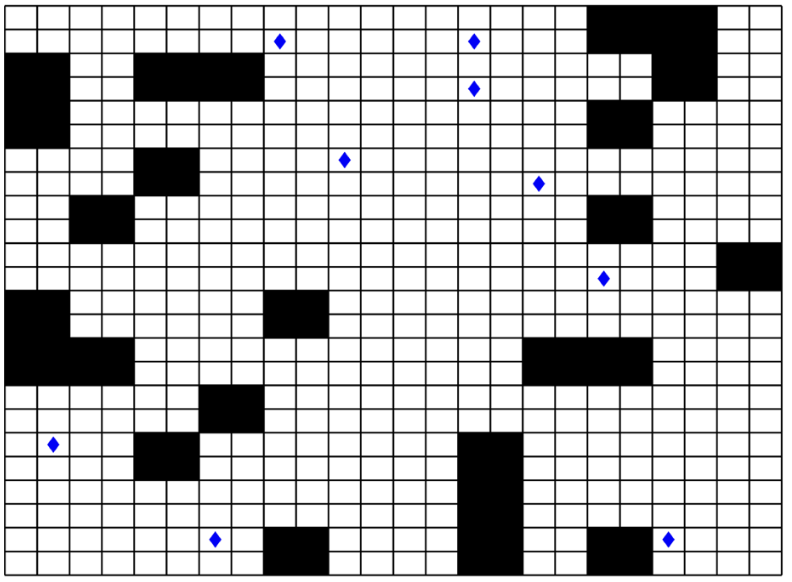
\includegraphics[width=0.45\columnwidth]{fig/darp1.png}
	}
	\hspace{0.1em}
	\subfloat[DARP outcome - robots’ exclusive areas \label{fig:darp2}]{
		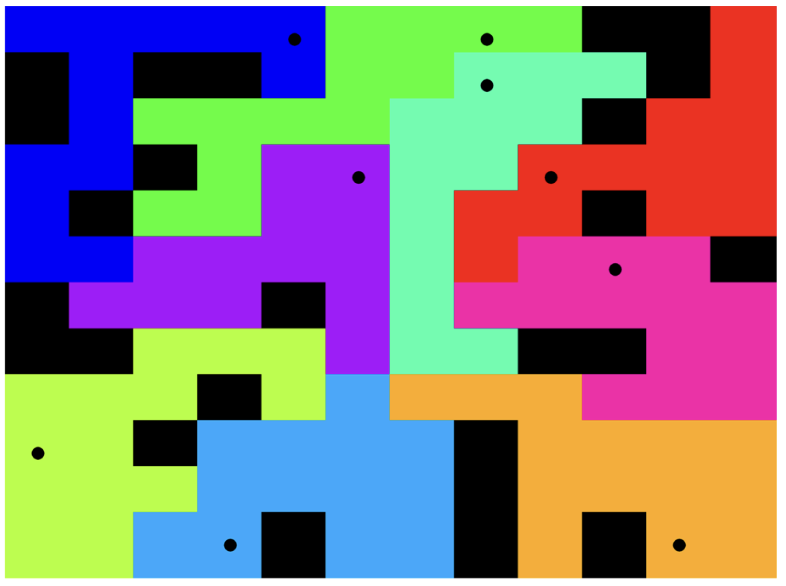
\includegraphics[width=0.45\columnwidth]{fig/darp2.png}
	}
	\\ % Line break for second row
	% Second row of subfigures
	\subfloat[Constructing Minimum Spanning Trees for each one of the robots sets \label{fig:darp3}]{
		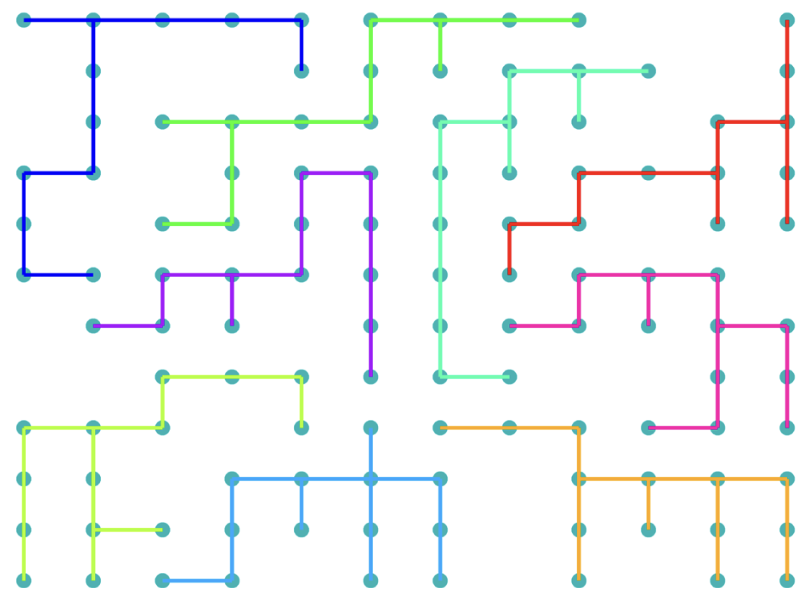
\includegraphics[width=0.45\columnwidth]{fig/darp3.png}
	}
	\hspace{0.1em}
	\subfloat[Final Paths, designed to circumnavigate the MSTs \label{fig:darp4}]{
		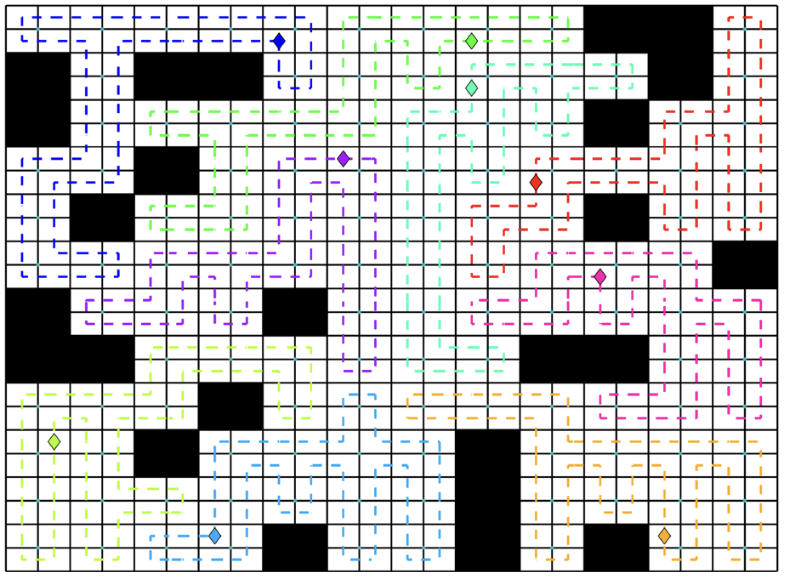
\includegraphics[width=0.45\columnwidth]{fig/darp4.png}
	}
	\caption{DARP+STC Proposed Approach, sample execution with 24x24 grid size, 9 robots and 100 obstacles  \cite{kapoutsisdarp}}
	\label{fig:darp_all}
\end{figure*}

There are $n_r$ robots, with $L_i$ being the robot sets for the $i_{th}$ robot. A selection $L_1, L_2, . . . , L_{n_r}$ poses an optimal solution for the mCPP, iff

\begin{itemize}
	\item $L_i \cap L_j = \emptyset, \quad \forall i, j \in \{1, \ldots, n_r\}, \, i \neq j$
	\item $\bigcup_{i=1}^{n_r} L_i = L$
	\item $\lvert L_1 \rvert \approx \lvert L_2 \rvert \dots \lvert L_{n_r} \rvert$
	\item $L_i \text{ is connected}, \quad \forall i \in \{1, \ldots, n_r\}$
	\item $\chi_i(t_0) \in L_i$
\end{itemize}

The first condition ensures that each cell is assigned exclusively to one robot’s set, enforcing a non-backtracking property in the resulting solution. The second condition specifies that the union of all \(L_i\) sets must cover every unblocked cell within the area, fulfilling the fundamental coverage requirement of completeness. The third condition focuses on maximizing the use of multi-robot dynamics by ensuring that the number of cells \(|L_i|\) in each robot’s set is approximately equal. The fourth condition mandates that each robot’s set \(L_i\) should consist of compact and contiguous cells, forming a cohesive sub-region. This guarantees a fair division and enables seamless navigation within spatially connected areas, preventing robots from spending unnecessary time traveling between disjoint regions. Finally, the fifth condition requires that each robot’s initial position \(\chi_i(t_0)\) is located within its assigned set \(L_i\), ensuring zero preparation time and minimizing energy consumption. Any algorithm capable of constructing the \(L_i\) sets while satisfying these five conditions can be combined with the STC algorithm to produce optimal solutions for the original mCPP problem.

Regarding the existence of such solutions, it has been proven that a fair partition, not restricted to convex regions, always exists for any polygon and any number of partitions. However, the variation of the problem considered here includes an additional condition: the requirement for each partition to contain a specified arbitrary point within the polygon. This added constraint makes the problem dependent on the arrangement of these arbitrary points and means a solution does not always exist. The overall formulation and proposed algorithm address cases where at least one optimal solution is guaranteed to exist.

In the algorithm, until all area division objectives are met, do:
\begin{enumerate}
	\item Assign every \((x, y)\) cell to a robot according to:
	\[
	A(x, y) = \argmin E_i(x, y)
	\]
	Here, $E_i$ is the evaluation matrix for Robot $i$ and  $E_i(x, y)$  is the reachability from $(x, y)$ and the initial position of robot $i$.
	\item For each \(i\)-th robot, where \(i \in \{1, \ldots, N\}\), perform the following steps:
	\begin{enumerate}
		\item Calculate \(k_i\), where $k_i = \lvert L_i \rvert$
		\item Update \(m_i \gets m_i + \eta(k_i - f)\), where $m_i$ is a scalar correction factor for the $i^{th}$ robot, and $f$ denotes the global fair share.
		\item Calculate the connectivity matrix \(C_i\).
		\item Update \(E_i \gets C_i \odot m_i E_i\).
	\end{enumerate}
\end{enumerate}

After the desired area division is achieved, we use Spanning Tree Coverage (STC) algorithm to produce the optimal path for each robot, in order to achieve full coverage of the area of interest.

\section{Drone Swarms}
\rhead{Drone Swarms}
\label{DroneSwarms}

Underwater drones, also known as Unmanned Underwater Vehicles (UUVs), have found significant applications in both civilian and military domains. These versatile vehicles are used in tasks ranging from deep-sea exploration to military operations. A notable area of innovation is \textbf{multi-agent Coverage Path Planning (mCPP)}, which focuses on optimizing the coverage of a defined area using multiple coordinated UUVs. Below are key applications of UUVs leveraging mCPP, supported by real-world examples.

\begin{itemize}
	\item \textbf{Military Applications:}
	\begin{itemize}
		\item \textbf{Mine Countermeasures:}  
		UUVs have been extensively used for mine detection and removal. For instance:
		\begin{itemize}
			\item During the Iraq War, the US Navy deployed UUVs to clear mines around the port of Umm Qasr \cite{RAND}.
			\item The REMUS UUV, a 3-foot-long robot, can clear mines in one square mile within 16 hours, a task that would take human divers over 21 days \cite{REMUS}.
		\end{itemize}
		
		\item \textbf{Data Collection and Reconnaissance:}  
		UUVs collect critical environmental data for military operations. Examples include:
		\begin{itemize}
			\item The Chinese Sea Wing (Haiyi) UUV, found near Indonesia’s Selayar Island in 2020, gathers data such as water temperature, salinity, and oxygen levels to map optimal submarine routes \cite{SeaWing}.
		\end{itemize}
		
		\item \textbf{Submarine Warfare and Surveillance:}  
		Advanced UUVs perform key roles in submarine warfare. For example:
		\begin{itemize}
			\item The Proteus UUV, developed by Huntington Ingalls Industries, utilizes synthetic aperture sonar to identify and neutralize underwater targets. This capability was demonstrated during the 2018 Advanced Naval Technology exercises \cite{Proteus}.
		\end{itemize}
		
		\item \textbf{Multi-Domain Operations:}  
		UUVs with trans-medium capabilities, such as China’s flying submarine drones, extend mCPP applications to both underwater and aerial missions \cite{Harbin2022}.
	\end{itemize}
	
	\item \textbf{Deep-Sea Exploration and Research:}
	\begin{itemize}
		\item \textbf{Mapping and Sample Collection:}  
		UUVs map the ocean floor and collect samples efficiently. Examples include:
		\begin{itemize}
			\item The \textit{Sentry} UUV by the Woods Hole Oceanographic Institution, which can map the seabed at depths of up to 6,000 meters \cite{WHOI}.
		\end{itemize}
		
		\item \textbf{Biodiversity Studies:}  
		UUVs assist in exploring and monitoring underwater ecosystems:
		\begin{itemize}
			\item Researchers have used UUVs to collect samples for studying the microplastic content of ocean floors and assess the health of deep-sea ecosystems \cite{DeepSea2021}.
		\end{itemize}
		
		\item \textbf{Exploration in Extreme Environments:}  
		UUVs are critical for operations in high-pressure environments:
		\begin{itemize}
			\item Bio-inspired soft robots capable of operating in the Mariana Trench have been used for deep-sea exploration and environmental monitoring \cite{Mariana2021}.
		\end{itemize}
	\end{itemize}
	
	\item \textbf{Ecosystem Monitoring and Rehabilitation:}
	\begin{itemize}
		\item \textbf{Water Quality Monitoring:}  
		UUVs are used to monitor and manage water ecosystems. Examples include:
		\begin{itemize}
			\item Duro AUS UUVs deployed in New York City's Randall's Island Park Alliance to monitor wetland health in the East and Harlem Rivers.
		\end{itemize}
		
		\item \textbf{River and Estuary Restoration:}  
		UUVs support environmental rehabilitation initiatives:
		\begin{itemize}
			\item The Bronx River Alliance uses UUVs to monitor and rejuvenate river ecosystems, helping to restore wildlife and improve water quality.
		\end{itemize}
	\end{itemize}
\end{itemize}

\noindent As advancements in robotics, artificial intelligence, and communication technologies continue to advance, the integration of mCPP in UUV operations is expected to expand, enabling transformative applications across military, scientific, and environmental domains.

\noindent This study investigates the application of compositional runtime enforcement in underwater robotic swarms, evaluating its performance in comparison to the conventional monolithic approach. The research focuses on integrating runtime enforcement into a Multi-Robot Coverage Path Planning (MRCPP) algorithm tailored for mapping underwater vegetation in seagrass beds. By analyzing both methods, the study seeks to determine their influence on the algorithm's efficiency, scalability, and flexibility in dynamic underwater conditions.

\begin{figure}[htb]
	\centering
	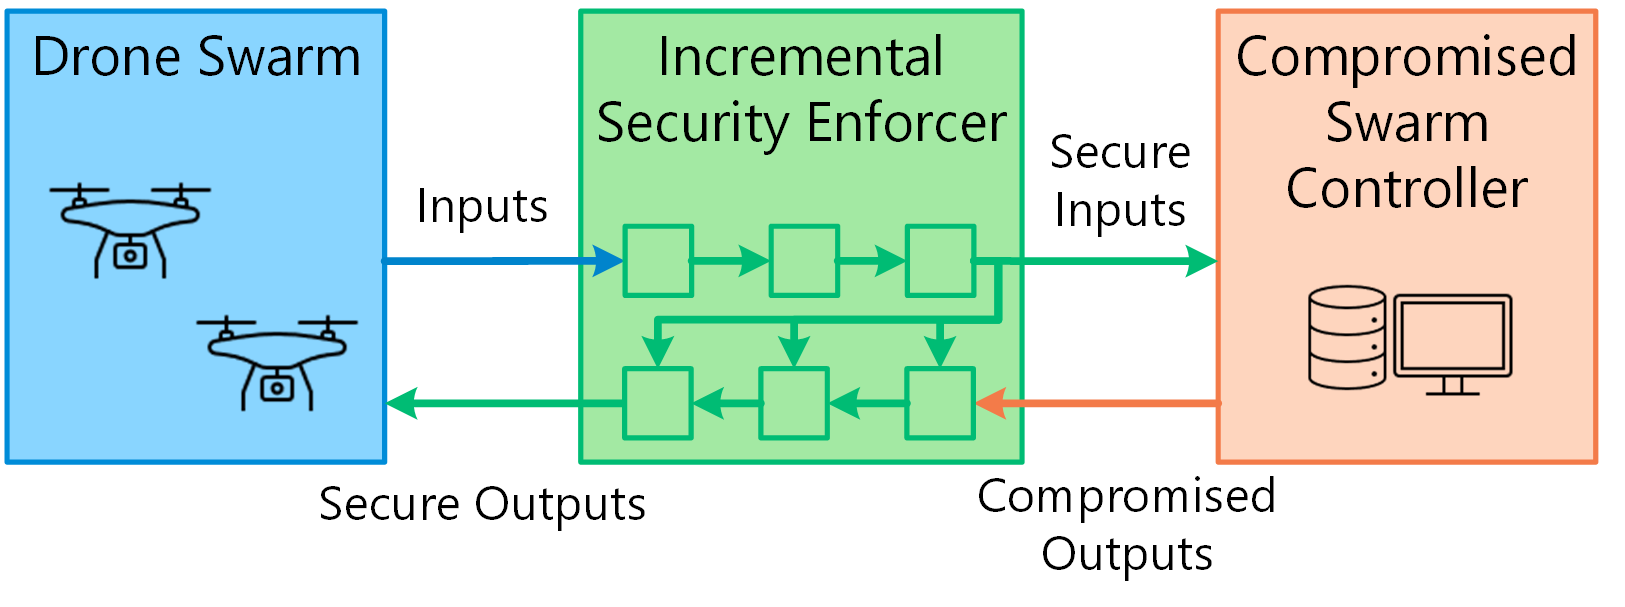
\includegraphics[width=0.94\linewidth]{fig/drone-system2.png}
	\caption{System diagram of incremental enforcement for a drone swarm.}
	\label{fig:drone-system}
\end{figure} 


\section{Attack On Drones}
\rhead{Attack On Drones}
\label{AttackOnDrones}

While underwater drones offer significant benefits in exploration, research, and military applications, they are not immune to threats from malicious actors. Recent work by Yaacoub et al. in \cite{yaacoub2020security} surveys a range of attacks on robotic systems. Underwater drones are particularly vulnerable to interference and manipulation due to their reliance on acoustic communication and complex navigation systems. For instance, acoustic jamming and spoofing attacks can disrupt communication and navigation, leading to miscoordination or loss of control \cite{westerlund2019drone}. Additionally, acoustic or magnetic interference can trigger emergency behaviors, such as premature surfacing or drifting \cite{Abunada2020}, and prevent the relay of vital status and control signals \cite{Valianti2021}. This disruption in communication between drones and the central controller can lead to unsafe outcomes, including collisions, mission failure, or environmental damage.

Hardware vulnerabilities, such as tampered communication modules or sensor systems \cite{belous2020hardware}, provide opportunities for attackers to inject, intercept, or alter control commands. Such attacks can force underwater drones to violate operational boundaries, collide with obstacles, or fail to execute their intended tasks.

In this work, we consider five potential attacks on an underwater drone swarm's coordinated operation:
\begin{itemize}
	\item[A1] \emph{Boundary Breach} \textit{(Injection and Alteration)}: where the attacker manipulates control signals to force drone(s) to leave their designated operational area, potentially breaching restricted zones or damaging sensitive ecosystems.
	\item[A2] \emph{Overwhelm Inputs} \textit{(Injection and Alteration)}: an attack where drone(s) are overloaded with conflicting or erroneous control signals, leading to erratic behavior or mission disruption.
	\item[A3] \emph{Block Control Signals} \textit{(Jamming)}: any attack that disrupts acoustic or RF communication, preventing updated control signals from reaching one or more drone(s) in the swarm.
	\item[A4] \emph{Drain Power} \textit{(Injection and Alteration)}: where the attacker commands drones to perform energy-intensive tasks, such as high-speed maneuvers or prolonged thruster usage, depleting their batteries prematurely.
	\item[A5] \emph{Pressure Limit Violation}  \textit{(Injection and Alteration)}: an attack where an adversary disrupts the simultaneous execution of pressure limit monitoring and ascent actions. This could cause drones to remain at unsafe depths, risking structural failure due to high pressure, or to ascend improperly, compromising mission integrity or safety.
\end{itemize}

We categorize these attacks into common types: \textit{jamming} and \textit{injection and alteration}. \textit{Injection and alteration} attacks involve the addition or manipulation of control packets, while \textit{jamming} attacks remove or block communication packets. To mitigate these threats, we develop robust policies enforced through a compositional runtime enforcement framework tailored to underwater drone operations.


\section{Mitigation with Enforcement}
\rhead{Mitigation with Enforcement}
\label{MitigationwithEnforcement}

This work defines a series of security policies to mitigate attacks on underwater drones. These policies are enforced through a runtime enforcement framework to ensure safe and secure operation, even in the presence of malicious interference. The inputs and outputs for each drone are defined as follows:

\begin{itemize}
	\item Inputs ($I$): $\lbrace \mathsf{left\_boundary}, \mathsf{right\_boundary}, \mathsf{down\_boundary}, \mathsf{up\_boundary}, \mathsf{rpm\_limit}, \mathsf{pressure\_limit} \rbrace$ (signals from the plant to the controller).
	\item Outputs ($O$): $\lbrace \mathsf{up}, \mathsf{down}, \mathsf{right}, \mathsf{left}, \mathsf{rpm\_up}, \mathsf{rpm\_down}, \mathsf{ascent} \rbrace$ (control actions sent from the controller to the plant).
\end{itemize}

The following policies correspond to the identified attacks and define mitigation strategies:

\begin{itemize}
	\item \textbf{Policy $\varphi_1$: Boundary Breach (Prevents A1)}  
	This policy ensures that drones do not violate predefined operational boundaries. It enforces the following:
	\begin{itemize}
		\item $\mathsf{left\_boundary}$ and $\mathsf{left}$ cannot occur simultaneously.
		\item $\mathsf{right\_boundary}$ and $\mathsf{right}$ cannot occur simultaneously.
		\item $\mathsf{down\_boundary}$ and $\mathsf{down}$ cannot occur simultaneously.
		\item $\mathsf{up\_boundary}$ and $\mathsf{up}$ cannot occur simultaneously.
	\end{itemize}
	
	\item \textbf{Policy $\varphi_2$: Conflicting Signals (Prevents A2)}  
	This policy ensures no simultaneous conflicting control signals are sent to the drone. It enforces the following:
	\begin{itemize}
		\item $\mathsf{left}$ and $\mathsf{right}$ cannot occur simultaneously.
		\item $\mathsf{up}$ and $\mathsf{down}$ cannot occur simultaneously.
		\item $\mathsf{rpm\_up}$ and $\mathsf{rpm\_down}$ cannot occur simultaneously.
	\end{itemize}
	
	\item \textbf{Policy $\varphi_3$: Block Control Signals (Prevents A3)}  
	This policy mandates that drones ascend to the surface when control signals are not received for a specific time threshold (5 seconds). It enforces:
	\begin{itemize}
		\item If no input or output signals are received, and the timer exceeds 5 seconds, then the drone ascends to the surface.
	\end{itemize}
	
	\item \textbf{Policy $\varphi_4$: Drain Batteries (Prevents A4)}  
	This policy ensures that the $\mathsf{rpm\_up}$ signal does not occur simultaneously with $\mathsf{rpm\_limit}$. It enforces:
	\begin{itemize}
		\item $\mathsf{rpm\_up}$ and $\mathsf{rpm\_limit}$ cannot occur simultaneously.
	\end{itemize}
	
	\item \textbf{Policy $\varphi_5$: Pressure Limit and Ascent Coordination (Prevents A5)}  
	This policy ensures that $\mathsf{pressure\_limit}$ and $\mathsf{ascent}$ occur simultaneously. It enforces:
	\begin{itemize}
		\item $\mathsf{pressure\_limit}$ and $\mathsf{ascent}$ must occur simultaneously.
	\end{itemize}
\end{itemize}

These policies collectively address key threats to underwater drones and ensure secure and reliable operations in dynamic and potentially adversarial environments.

\subsubsection{Policy $\varphi_{1}$ mitigating attack A1, \emph{Boundary Breach}}

The \emph{Boundary Breach} attack occurs when a drone is instructed to violate predefined airspace boundaries or the separation limits between drones. To mitigate this, Policy $\varphi_1$ ensures that the drone operates within its allowed 2D workspace while moving in four primary directions: left, right, up, and down. The drone is prevented from breaching boundaries or failing to move when expected. Specifically, for the \textbf{left} direction:

\begin{itemize}
	\item If the drone attempts to move left while already at the left boundary (\texttt{left\_boundary} $\land$ \texttt{left}), it is considered a violation, and the drone's left movement is disabled (\texttt{left := 0}).
	\item If the drone fails to move left when not at the left boundary ($\neg$ \texttt{left\_boundary} $\land$ $\neg$ \texttt{left}), the policy forces left movement (\texttt{left := 1}).
\end{itemize}

The same logic applies for the other directions (\textbf{right}, \textbf{up}, and \textbf{down}) with their respective boundary conditions (\texttt{right\_boundary}, \texttt{up\_boundary}, \texttt{down\_boundary}). This policy ensures that the drone adheres to boundary constraints, preventing it from breaching airspace limits or failing to navigate appropriately within the defined 2D area.


\begin{figure}[H]
	\centering
	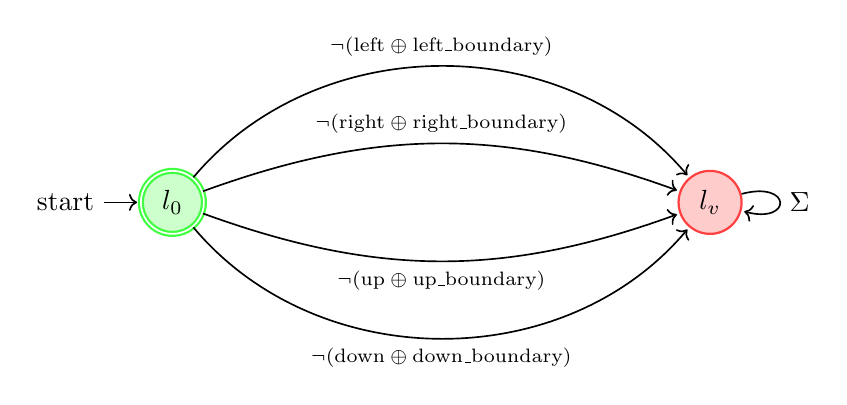
\begin{tikzpicture}[->,shorten >=1pt,auto,node distance=4cm,semithick]
		
		% Styles for the states
		\tikzstyle{state}=[circle,thick,draw=green!75,fill=green!20,minimum size=8mm]
		\tikzstyle{accepting state}=[state, double]
		\tikzstyle{violation state}=[circle,thick,draw=red!75,fill=red!20,minimum size=8mm]
		
		% Nodes for the DFA
		\node[accepting state,initial] (l0) {$l_0$};
		\node[violation state] (lv) [right=6cm of l0] {$l_v$};
		
		% Transitions from l0 to lv with adjusted label placement
		\path
		(l0) edge[bend left=50] node[above] {\scriptsize $\neg (\text{left} \oplus \text{left\_boundary})$} (lv)
		(l0) edge[bend left=20] node[above] {\scriptsize $\neg (\text{right} \oplus \text{right\_boundary})$} (lv)
		(l0) edge[bend right=20] node[below] {\scriptsize $\neg (\text{up} \oplus \text{up\_boundary})$} (lv)
		(l0) edge[bend right=50] node[below] {\scriptsize $\neg (\text{down} \oplus \text{down\_boundary})$} (lv)
		
		% Self-loop on violation state
		(lv) edge[loop right] node {$\Sigma$} (lv);
		
	\end{tikzpicture}
	\caption{Automaton for policy $\varphi_{1}$ which prevents a drone from breaching its boundary}
	\label{fig:p1}
\end{figure}

\subsubsection{Policy $\varphi_{2}$ mitigating attack A2, \emph{Overwhelm Inputs}}

In attack A2, \emph{Overwhelm Inputs}, the attacker sends conflicting control signals to the drone. Policy $\varphi_{2}$ is designed such that simultaneously present conflicting controls cause violation. The synthesised enforcer will therefore suppress one of these conflicting signals to ensure the drone is not overwhelmed.

\begin{figure}[H]
	\centering
	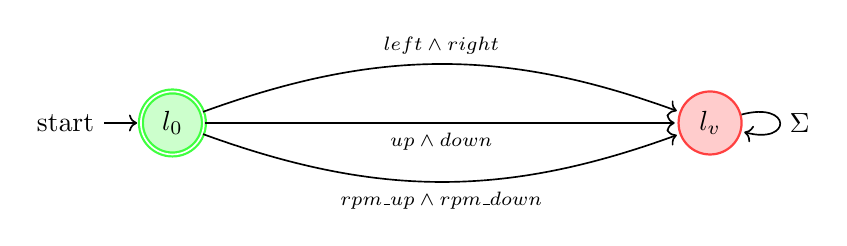
\begin{tikzpicture}[->,shorten >=1pt,auto,node distance=4cm,semithick]
		% Styles for the states
		\tikzstyle{state}=[circle,thick,draw=green!75,fill=green!20,minimum size=8mm]
		\tikzstyle{accepting state}=[state, double]
		\tikzstyle{violation state}=[circle,thick,draw=red!75,fill=red!20,minimum size=8mm]
		
		% Nodes for the DFA
		\node[accepting state,initial] (l0) {$l_0$};
		\node[violation state] (lv) [right=6cm of l0] {$l_v$};
		
		% Transitions from l0 to lv with adjusted label placement
		\path
		(l0) edge[bend left=20] node[above] {\scriptsize $left \land right$} (lv)
		(l0) edge[bend left=0] node[below] {\scriptsize $up \land down$} (lv)
		(l0) edge[bend right=20] node[below] {\scriptsize $rpm\_up \land rpm\_down$} (lv)
		
		% Self-loop on violation state
		(lv) edge[loop right] node {$\Sigma$} (lv);
	\end{tikzpicture}
	\caption{Automaton for policy $\varphi_{2}$ which prevents overwhelming of the inputs}
	\label{fig:p2}
\end{figure}


\subsubsection{Policy $\varphi_{3}$ mitigating attack A3, \emph{Block Control Signals}}

The attack A3, \emph{ Block Control Signals}, which jams signals prevents the drone from getting updated controls. This could result in it continuing to climb or move in undesirable ways. The policy detects if no control signals are sent in any 5-second period. The drone is then brought to the surface using the \texttt{ascent} signal.


\begin{figure}[H]
	\centering
	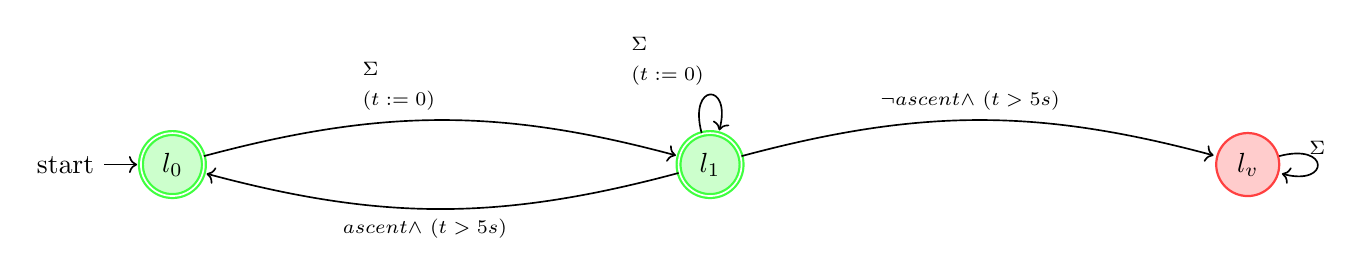
\begin{tikzpicture}[->,shorten >=1pt,auto,node distance=4cm,semithick]
		
		% Styles for the states
		\tikzstyle{state}=[circle,thick,draw=green!75,fill=green!20,minimum size=8mm]
		\tikzstyle{accepting state}=[state, double]
		\tikzstyle{violation state}=[circle,thick,draw=red!75,fill=red!20,minimum size=8mm]
		
		% Nodes for the DFA
		\node[accepting state,initial] (l0) {$l_0$};
		\node[accepting state] (l1) [right=6cm of l0] {$l_1$};
		\node[violation state] (lv) [right=6cm of l1] {$l_v$};
		
		% Transitions
		\path
		% Transition from l0 to l1
		(l0) edge[bend left=15] node[above] {\scriptsize \parbox{2cm}{$\Sigma$ \\ ($t := 0$)}} (l1)
		
		% Transition from l1 to l0
		(l1) edge[bend left=15] node[below] {\scriptsize \parbox{2.5cm}{$ascent \land$ $(t > 5s)$}} (l0)
		
		% Self-loop on l1
		(l1) edge[loop above] node[above] {\scriptsize \parbox{2cm}{$\Sigma$ \\ ($t := 0$)}} (l1)
		
		% Transition from l1 to lv
		(l1) edge[bend left=15] node[above] {\scriptsize \parbox{2.5cm}{$\neg ascent \land$ $(t > 5s)$}} (lv)
		
		% Self-loop on lv
		(lv) edge[loop right] node[above] {\scriptsize $\Sigma$} (lv);
		
	\end{tikzpicture}
	\caption{Automaton for policy $\varphi_{3}$ which ensures safe transitions based on timeout and ascent conditions.}
	\label{fig:p3}
\end{figure}


\subsubsection{Policy $\varphi_{4}$ mitigating attack A4, \emph{Drain Batteries}}

Attack A4, \emph{Drain Batteries}, involves injection or alteration of signals to increase the drone's RPM beyond the efficiency threshold, which is crucial for maintaining optimal flight endurance during the QR display. Although higher RPM allows faster movement, it significantly reduces efficiency, causing the battery to deplete more rapidly. To mitigate this, an RPM limit is enforced. Policy $\varphi_{4}$ is a simple policy which prevents $rpm\_up$ signal when $rpm\_limit$ is active.

\begin{figure}[H]
	\centering
	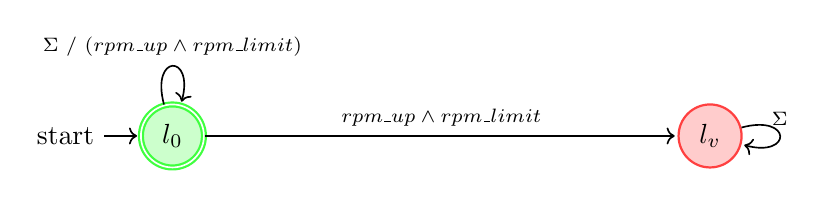
\begin{tikzpicture}[->,shorten >=1pt,auto,node distance=5cm,semithick]
		
		% Styles for the states
		\tikzstyle{state}=[circle,thick,draw=green!75,fill=green!20,minimum size=8mm]
		\tikzstyle{accepting state}=[state, double]
		\tikzstyle{violation state}=[circle,thick,draw=red!75,fill=red!20,minimum size=8mm]
		
		% Nodes for the DFA
		\node[accepting state,initial] (l0) {$l_0$};
		\node[violation state] (lv) [right=6cm of l0] {$l_v$};
		
		% Transitions
		\path
		% Self-loop on l0
		(l0) edge[loop above] node[above] {\scriptsize $\Sigma$ / ($rpm\_up \land rpm\_limit$)} (l0)
		
		% Transition from l0 to lv
		(l0) edge[bend left=0] node[above] {\scriptsize $rpm\_up \land rpm\_limit$} (lv)
		
		% Self-loop on lv
		(lv) edge[loop right] node[above] {\scriptsize $\Sigma$} (lv);
		
	\end{tikzpicture}
	\caption{Automaton for policy $\varphi_{4}$ which ensures safe RPM limits to prevent battery drain.}
	\label{fig:p4}
\end{figure}

\subsubsection{Policy $\varphi_{5}$ mitigating attack A5, \emph{Pressure Limit Violation}}

Attack A5, \emph{Pressure Limit Violation}, occurs when an adversary prevents the drone from initiating ascent even when the pressure limit is reached. This attack exploits the safety mechanism designed to protect the drone from operating at unsafe depths, potentially leading to structural damage or mission failure. To mitigate this, Policy $\varphi_{5}$ ensures that the drone immediately triggers the \texttt{ascent} signal whenever the \texttt{pressure\_limit} condition is met, preventing prolonged exposure to high-pressure environments. This simple policy blocks operations that ignore the \texttt{pressure\_limit} condition, ensuring safe and reliable behavior.

\begin{figure}[H]
	\centering
	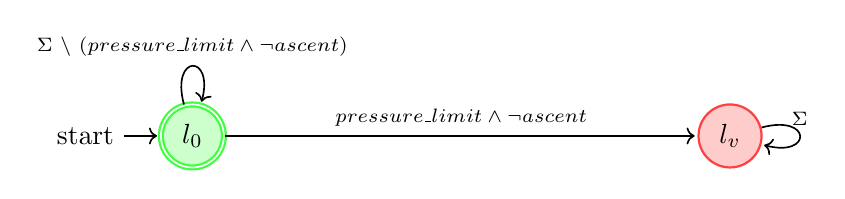
\begin{tikzpicture}[->,shorten >=1pt,auto,node distance=5cm,semithick]
		
		% Styles for the states
		\tikzstyle{state}=[circle,thick,draw=green!75,fill=green!20,minimum size=8mm]
		\tikzstyle{accepting state}=[state, double]
		\tikzstyle{violation state}=[circle,thick,draw=red!75,fill=red!20,minimum size=8mm]
		
		% Nodes for the DFA
		\node[accepting state,initial] (l0) {$l_0$};
		\node[violation state] (lv) [right=6cm of l0] {$l_v$};
		
		% Transitions
		\path
		% Self-loop on l0
		(l0) edge[loop above] node[above] {\scriptsize $\Sigma$ \textbackslash\ ($pressure\_limit \land \neg ascent$)} (l0)
		
		% Transition from l0 to lv
		(l0) edge[bend left=0] node[above] {\scriptsize $pressure\_limit \land \neg ascent$} (lv)
		
		% Self-loop on lv
		(lv) edge[loop right] node[above] {\scriptsize $\Sigma$} (lv);
		
	\end{tikzpicture}
	\caption{Automaton for policy $\varphi_{5}$ which ensures ascent is triggered when the pressure limit is reached.}
	\label{fig:p5}
\end{figure}











  \newpage
%  %\newpage\null\newpage
  
\chapter{Implementation and Evaluation}
\graphicspath{{Chapter_4/Vector/}{Chapter_4/}}

To assess the effectiveness of the proposed incremental serial composition approach, we developed a straightforward simulator for a multi-drone system. The simulator is based on the structure depicted in Figure~\ref{fig:drone-system}, incorporating a controller, enforcer, and the drone itself. This implementation enables a direct comparison between the traditional monolithic approach and the incremental serial composition method. For evaluation, we intentionally introduce faults into the simulated controller, compelling the enforcer to make consistent edits. This setup allows us to measure and analyze the time required for the enforcer to execute its corrections effectively.


The software tool \textit{easy-rte} \cite{8859335} was used to produce enforcers for this implementation. The tool provides support for monolithic composition, which we use to produce our monolithic enforcers. Additionally, \textit{easy-rte-incremental} \cite{10047915} was used to produce the serial implementation.

To ensure the enforcers actively intervene, the controller was intentionally compromised. To illustrate the effect of progressively complex compositions, we began with a single $\varphi_1$ policy, designed to counteract the boundary breach attack (A1) for the first drone. Additional policies, $\varphi_2$, $\varphi_3$, $\varphi_4$, and $\varphi_5$, were then incrementally incorporated, addressing attacks A2, A3, A4, and A5, respectively, across the drones.

Therefore we created five enforcers for both monolithic and serial compositions to satisfy the following:
\begin{itemize}
	\item[] $E_{\varphi1}$: enforces $\varphi_1$
	\item[] $E_{\varphi2}$: enforces $\varphi_1$, and $\varphi_2$
	\item[] $E_{\varphi3}$: enforces $\varphi_1 $, $ \varphi_2 $, and $\varphi_3$
	\item[]$E_{\varphi4}$: enforces $\varphi_1 $, $ \varphi_2 $, $ \varphi_3 $, and $ \varphi_4$
	\item[] $E_{\varphi5}$: enforces $\varphi_1 $, $ \varphi_2 $, $ \varphi_3 $, $ \varphi_4 $, and $ \varphi_{5}$ 
\end{itemize}

Monolithic compositions were composed into a single policy first and are denoted $\varphi_{1M}$, $\varphi_{2M}$, ..., $\varphi_{55M}$. These are then synthesized into enforcers denoted $E_{\varphi_{1M}}$. Serial compositions are denoted $E_{\varphi_{1S}}$, $E_{\varphi_{2S}}$, ..., $E_{\varphi_{5S}}$.

\section{Evaluation Parameters}
\rhead{Evaluation Parameters}
\label{EvaluationParameters}

xmx





% \newpage
\lhead{}
\rhead{\footnotesize Appendix}
\appendix
\addcontentsline{toc}{chapter}{Appendix}

%%%%% Creating Appendix A
	\chapter{}
	\label{appendix0}
		\graphicspath{{Appendices/Vector/}{Appendices/}}
	%%% Lauricella's Hypergeometric Functions
	%%%%%
\section*{Title of Appendix}
%%%%%%%%%%%%%%%%%%%%%%%%%%%%%%%%%%% 
%%%%%%%%%%%% Complete System Diagram
%%%%%%%%%%%%%%%%%%%%%%%%%%%%%%%%%%%

xxxxxx xxxxxx xxxxxx xxxxxx xxxxxx xxxxxx xxxxxx xxxxxx xxxxxx xxxxxx xxxxxx xxxxxx xxxxxx xxxxxx xxxxxx xxxxxx xxxxxx xxxxxx xxxxxx xxxxxx xxxxxx xxxxxx xxxxxx xxxxxx xxxxxx xxxxxx xxxxxx xxxxxx xxxxxx xxxxxx xxxxxx xxxxxx xxxxxx xxxxxx xxxxxx xxxxxx xxxxxx xxxxxx xxxxxx xxxxxx xxxxxx xxxxxx xxxxxx xxxxxx.

\begin{align}
y=\alpha\,x+n
\end{align} 
%\input{Appendices/appendix1}
%\input{Appendices/appendix2}
%\input{Appendices/appendix3}
  \newpage
  \singlespacing
%   %\newpage\null\newpage
\pagestyle{fancy}
\fancyhf{}
\rhead{\fancyplain{}{Publications}}
\cfoot{\fancyplain{}{\thepage}}
  \addcontentsline{toc}{chapter}{Publications}
  	\chapter*{Publications}
	\graphicspath{{Publications/Vector/}{Publications/}}
	\noindent{\bf {Journal Publications}}
	\begin{enumerate}
		\item{ }
		\item{ }
		\item{ }
		
		
		
	\end{enumerate}
	\noindent{\bf{Conference Publication}}
	\begin{enumerate}
		\item 
		\item
		
	\end{enumerate}
  \newpage
\singlespacing
\pagestyle{fancy}
\fancyhf{}
\rhead{\fancyplain{}{Bibliography}}
\cfoot{\fancyplain{}{\thepage}}
\addcontentsline{toc}{chapter}{Bibliography}
\bibliographystyle{IEEEtran}
\bibliography{IEEEabrv,bibliography}


\end{document}

